%%%%%%%%%%%%%%%%%%%%%%%%%%%%%%%%%%%%%%%%%
% TMDEI Dissertation
% LaTeX Template
% Version 0.1 (Dec/2015)
%
% Adapted to TMDEI/ISEP style (Dec/2015) by
%  Nuno Pereira (nap@isep.ipp.pt) and
%  Paulo Baltarejo (pbs@isep.ipp.pt)
%
% Based on MastersDoctoralThesis Version 1.2 by Vel (vel@latextemplates.com) and
% Johannes Böttcher, downloaded from (21/11/15):
% http://www.LaTeXTemplates.com
%
% This template is originally based on a template by:
% Steve Gunn (http://users.ecs.soton.ac.uk/srg/softwaretools/document/templates/)
% Sunil Patel (http://www.sunilpatel.co.uk/thesis-template/)
%
% Template license:
% CC BY-NC-SA 3.0 (http://creativecommons.org/licenses/by-nc-sa/3.0/)
%
%%%%%%%%%%%%%%%%%%%%%%%%%%%%%%%%%%%%%%%%%

%----------------------------------------------------------------------------------------
%	PACKAGES AND OTHER DOCUMENT CONFIGURATIONS
%----------------------------------------------------------------------------------------

\documentclass[
10pt, % The default document font size, options: 10pt, 11pt, 12pt
%twoside,
oneside, % Two side (alternating margins) for binding by default, uncomment to switch to one side (for drafting/reading purposes)
%english, % english for English;
portuguese,% for Portuguese; delete temporary files if you change language (e.g. 'make clean; make')
singlespacing, % Single line spacing, alternatives: onehalfspacing or doublespacing (for drafting/reading purposes)
%draft, % Uncomment to enable draft mode (no pictures, no links, overfull hboxes indicated)
%nolistspacing, % If the document is onehalfspacing or doublespacing, uncomment this to set spacing in lists to single
liststotoc, % Uncomment to add the list of figures/tables/etc to the table of contents (not recommended)
%toctotoc, % Uncomment to add the main table of contents to the table of contents (not recommended)
parskip, % Add space between paragraphs (recommended)
%nohyperref, % Uncomment to not load the hyperref package (not recommended)
nohyperreflinkcolor, % hyperref links are not colored (comment to color links, for example to produce an electronic-only version)
headsepline, % Uncomment to get a line under the header
]{tmdei-style} % The class file specifying the document structure

\usepackage{subcaption}
\usepackage{rotating}
\usepackage{multicol}
\usepackage{soul}
\usepackage{tikz} % Required for creating graphics programmatically (can be removed if not used)
%\usetikzlibrary{arrows} % Required for fancy arrows in TiKZ graphics (can be removed if not used)
\usetikzlibrary{mindmap,trees}
\usepackage{pgfplots} % Required for drawing high--quality function plots (can be removed if not used)
\pgfplotsset{compat=newest}

%
% Next you have examples of admissable citation styles; we recomend using the authoryear-comp citation style (which resembles Harvard); don't forget to only uncomment one
%

% authoryear-comp: recommended citation style (e.g. (Buendía, 1860), (Buendía 1910, Arcadio 1940))
\usepackage[style=authoryear-comp,backend=biber]{biblatex} % Bibtex backend with the authoryear-comp citation style (authoryear citations, bibliography ordered alphabetically)
%\setlength\bibitemsep{.5\baselineskip}
% numeric citation style (e.g. [1], [1-3])
%\usepackage[style=numeric-comp,sorting=none,backend=biber]{biblatex} % Bibtex backend with the numeric-comp citation style (numeric citations, bibliography ordered by appearance)

% alphabetic citation style (e.g. [Buendía10], [Buendía10, Arcadio40])
%\usepackage[style=alphabetic,sorting=none,backend=biber]{biblatex} % Bibtex backend with the alphabetic citation style (alphabetic citations, bibliography ordered by appearance)
\addbibresource{mainbibliography.bib} % The filename of the bibliography

\makeglossaries % build the glossary

%----------------------------------------------------------------------------------------
%	THESIS INFORMATION
%----------------------------------------------------------------------------------------

\thesistitle{Natural Language Querying} % Your thesis title, this is used in the title, print it elsewhere with \ttitle

%\thesissubtitle{Uma abordagem ao problema das Interfaces de Linguagem Natural} % Your thesis title, this is used in the title, print it elsewhere with \tsubtitle

\author{Tiago Gabriel da Silva} % Your name, this is used in the title page, print it elsewhere with \authorname

\subjectarea{Sistemas Computacionais} % Specialization area (Computer Systems, Information and Knowledge Systems, Graphics, Systems and Multimedia, Software Engineering), used in the title page, print it elsewhere with \areaname

\supervisor{Prof. Doutor Paulo Gandra de Sousa} % Your supervisor's name, this is used in the title page, print it elsewhere with \supname

\cosupervisor{{Eng.\textordmasculine} Ricardo Magalhães} % Your co-supervisor's name, this is used in the title page, print it elsewhere with \cosupname (comment, if no co-supervisor)

\committeepresident{{Prof.\textordfeminine} Doutora Isabel Azevedo, DEI/ISEP} % Name of the president of the evaluation committee, print it elsewhere with \presidentname

\committeemembers{Prof. Doutor Nuno Escudeiro, DEI/ISEP} % Name of the evaluation committee members (up to four), print it elsewhere with \committee

\keywords{Indústria 4.0, Inteligência Artificial, Interfaces de Linguagem Natural, \textit{Machine Learning}, \textit{Manufacturing Execution System}} % Please define up to 6 keywords that better describe your work, print it elsewhere with \keywordnames

\university{\href{http://www.isep.ipp.pt}{Instituto Superior de Engenharia do Porto}} % Your university's name and URL, this is used in the title page and abstract, print it elsewhere with \univname

\department{\href{http://www.dei.isep.ipp.pt}{Departamento de Engenharia Informática}} % Your department's name and URL, this is used in the title page and abstract, print it elsewhere with \deptname

% \thesisdate{Porto, \today} % thesis date,  print it elsewhere with \tdate
\thesisdate{Porto, {\ifcase \month\or Janeiro\or Fevereiro\or Março\or Abril\or Maio\or Junho\or Julho\or Agosto\or Setembro\or Outubro\or Novembro\or Dezembro\fi \space de \number\year}
}

\hypersetup{pdftitle=\ttitle} % Set the PDF's title to your title
\hypersetup{pdfauthor=\authorname} % Set the PDF's author to your name
\hypersetup{pdfkeywords=\keywordnames} % Set the PDF's keywords to your keywords

% Variables
\def\companyname{Critical Manufacturing}
\def\productname{Critical Manufacturing MES}
\def\tbd{\hl{\textit{A definir}}}

\begin{document}

%----------------------------------------------------------------------------------------
%	FRONT MATTER
%----------------------------------------------------------------------------------------

% Include the frontmatter of your thesis here
% we include the glossary here (front matter is included with \input, so this command is as if it was in main.tex)
% Acrónimos
\newacronym{iot}{IoT}{\textit{Internet of Things}}
\newacronym{ios}{IoS}{\textit{Internet of Services}}
\newacronym{ihc}{IHC}{Interação Humano-Computador}
\newacronym{ia}{IA}{Inteligência Artificial}
\newacronym{pln}{PLN}{Processamento de Linguagem Natural}
\newacronym{mes}{MES}{\textit{Manufacturing Execution System}}
\newacronym{sql}{SQL}{\textit{Structured Query Language}}
\newacronym{uml}{UML}{\textit{Unified Modeling Language}}
\newacronym{ceo}{CEO}{\textit{Chief Executive Officer}}
\newacronym{cto}{CTO}{\textit{Chief Technical Officer}}
\newacronym{erp}{ERP}{\textit{Enterprise Resource Planning}}
\newacronym{cps}{CPS}{\textit{Cyber-Physical System}}
\newacronym{ffe}{FFE}{\textit{Fuzzy Front End}}
\newacronym{npd}{NPD}{\textit{New Product Development}}
\newacronym{ncd}{NCD}{\textit{New Concept Development}}
\newacronym{slp}{SLP}{\textit{Single Layer Perceptron}}
\newacronym{ilnbd}{ILNBD}{Interfaces de Linguagem Natural para Bases de Dados}
\newacronym{atn}{ATN}{\textit{Augmented Transition Network}}
\newacronym{xml}{XML}{\textit{Extensible Markup Language}}
% for defining plural form
% \newacronym[shortplural=aa,longplural=letters a]{a}{A}{the a}

\frontmatter % Use roman page numbering style (i, ii, iii, iv...) for the pre-content pages

\pagestyle{plain} % Default to the plain heading style until the thesis style is called for the body content

%----------------------------------------------------------------------------------------
%	TITLE PAGE
%----------------------------------------------------------------------------------------

\maketitlepage

%----------------------------------------------------------------------------------------
%	DEDICATION  (optional)
%----------------------------------------------------------------------------------------
\begin{dedicatory}
\tbd
\end{dedicatory}

%----------------------------------------------------------------------------------------
%	ABSTRACT PAGE
%----------------------------------------------------------------------------------------
\begin{abstract}

O paradigma de interação entre Homem e Máquina tem vindo a mudar nos últimos anos. Se ao longo das últimas décadas, o ser humano tem vindo a interagir com o computador através da escrita (linha de comandos) ou das interfaces gráficas, mais recentemente, surge a interação por linguagem natural. Como potenciar a comunicação entre o Homem e os sistemas usados diariamente, usando linguagem natural? Recorrendo ao Processamento de Linguagem Natural, um campo de estudo ligado à Inteligência Artificial, que pode envolver técnicas de \textit{Machine Learning} ou \textit{Deep Learning}, torna-se possível transformar a linguagem do ser humano numa representação adaptada aos sistemas computacionais. 

A presente tese debruça-se na conceção de uma abordagem que permita a consulta e apresentação de informação contida em armazéns de dados, recorrendo a linguagem natural. Neste âmbito, foi desenvolvido um protótipo que assenta sobre a abordagem conceptualizada. Assim, o intuito final é adaptar e usar a abordagem proposta no desenvolvimento dum módulo de linguagem natural para interface com o {\productname}, procurando aprimorar a usabilidade do sistema.

\end{abstract}

\begin{abstractotherlanguage}
The interaction paradigm between man and machine has been changing in the last years. Over the last decades, humans have been interacting with the computer through writing (command line) or graphical interfaces. Recently, emerges the interaction through natural language. How to enhance the communication between man and the system used on daily basis, by using natural language? The usage of Natural Language Processing, a field of study of Artificial Intelligence, which may involve Machine Learning or Deep Learning techniques, allows the transformation of human language into a representation adapted to computation systems.

This thesis focus on the design of an approach that allows to consult and present information stored in data warehouses, through usage of natural language. As result, a prototype has been developed by putting into practise the conceptualized approach. Thus, the main goal is to adapt and use the suggested approach in the development of a natural language module to interact with the {\productname}, thereby improving the system's usability.

\end{abstractotherlanguage}

%----------------------------------------------------------------------------------------
%	ACKNOWLEDGEMENTS (optional)
%----------------------------------------------------------------------------------------
\begin{acknowledgements}

O trabalho desempenhado ao longo de quase um ano não seria possível sem a presença de várias pessoas, as quais marcam a minha vida todos os dias, e das quais tenho apoio incondicional.

Quero agradecer aos meus pais, pela educação, pelo apoio, pelo incentivo e principalmente, pelos valores que me foram incutidos, que fizeram de mim a pessoa que sou hoje. Alguns anos conturbados passaram e hoje tudo faz sentido -- \textit{I'm in hell without you, cannot cope without you two, shocked at the world that I see}. Obrigado.

Agradeço aos meus amigos, por aturarem as minhas longas \inquotes{palestras}, por me ouvirem, na alegria e na tristeza, e por incentivarem o meu sucesso (por ordem alfabética): Diogo, Egídio, Francisco, Joel, Sérgio, Wilson. Grande abraço.

Para o Diogo, obrigado por seres o \textit{brother from another mother}. Ligeiramente picuinhas, eu sei, mas não precisamos de palavras.

Deixo o meu agradecimento ao Instituto Superior de Engenharia do Porto, em particular aos professores que acompanharam o meu percurso e que foram uma inspiração. 

Agradeço à Critical Manufacturing, em especial ao Engenheiro Ricardo Magalhães, pela incentivo dado neste projeto, pelas ideias e pelos desafios que se demonstraram difíceis, mas que com diálogo foram possíveis alcançar. 

Ainda no contexto Critical Manufacturing, quero também deixar o meu agradecimento a todas as pessoas com quem tive o prazer de trabalhar. Quero deixar um agradecimento especial ao Rui Santos, por ter sido o meu mentor na jornada CMF e por me ter \inquotes{dado asas}. Obrigado pelas longas conversas musicais, técnicas e dos momentos de riso. Com certeza que nos vamos cruzar, especialmente em muitos concertos! \textit{Rock On}!

Ao meu orientador, Doutor Paulo Gandra de Sousa, que confiou em mim e no desempenho deste trabalho, que se demonstrou preocupado quando não dava notícias (peço desculpa, professor) e me ajudou a traçar o caminho seguido neste trabalho.

E, como sou uma pessoa que deixa o melhor para o fim, agradeço à Patrícia, minha amiga, confidente, apoiante número um, psicóloga e ouvinte nas horas vagas. Sempre acreditaste em mim, e continuas a fazê-lo, e não há palavras suficientes para descrever a minha gratidão -- \textit{Love of my Life}.

A todos, o meu mais profundo obrigado!
\end{acknowledgements}

%----------------------------------------------------------------------------------------
%	LIST OF CONTENTS/FIGURES/TABLES PAGES
%----------------------------------------------------------------------------------------

\tableofcontents % Prints the main table of contents

\listoffigures % Prints the list of figures

\listoftables % Prints the list of tables

% \iflanguage{portuguese}{
% \renewcommand{\listalgorithmname}{Lista de Algor\'itmos}
% }{}
% \listofalgorithms % Prints the list of algorithms
% \addchaptertocentry{\listalgorithmname}

\iflanguage{portuguese}{
\renewcommand{\lstlistlistingname}{Lista de C\'odigo}
\renewcommand{\lstlistingname}{C\'odigo}
}{ 
\renewcommand{\lstlistlistingname}{List of Source Code}
\renewcommand{\lstlistingname}{C\'ode}
}
\lstlistoflistings
\addchaptertocentry{\lstlistlistingname}

%----------------------------------------------------------------------------------------
%	ABBREVIATIONS
%----------------------------------------------------------------------------------------
%\begin{abbreviations}{ll} % Include a list of abbreviations (a table of two columns)
%\textbf{LAH} & \textbf{L}ist \textbf{A}bbreviations \textbf{H}ere\\
%\textbf{WSF} & \textbf{W}hat (it) \textbf{S}tands \textbf{F}or\\
%\end{abbreviations}

%----------------------------------------------------------------------------------------
%	SYMBOLS
%----------------------------------------------------------------------------------------

%\begin{symbols}{lll} % Include a list of Symbols (a three column table)

$a$ & distance & \si{\meter} \\
$P$ & power & \si{\watt} (\si{\joule\per\second}) \\
%Symbol & Name & Unit \\

\addlinespace % Gap to separate the Roman symbols from the Greek

$\omega$ & angular frequency & \si{\radian} \\

\end{symbols}

%----------------------------------------------------------------------------------------
%	ACRONYMS
%----------------------------------------------------------------------------------------

\newcommand{\listacronymname}{List of Acronyms}
\iflanguage{portuguese}{
\renewcommand{\listacronymname}{Lista de Acr\'onimos}
}
% Use GLS
\glsresetall
\printglossary[title=\listacronymname,type=\acronymtype,style=long]

%----------------------------------------------------------------------------------------
%	DONE
%----------------------------------------------------------------------------------------

\mainmatter % Begin numeric (1,2,3...) page numbering
\pagestyle{thesis} % Return the page headers back to the "thesis" style


%----------------------------------------------------------------------------------------
%	MAIN BODY
%----------------------------------------------------------------------------------------

% Include the chapters of the thesis as separate folder for each chapter
% Uncomment the lines as you write the chapters

\chapter{Introdução}
\label{chap:Chapter1}
Num mercado crescentemente competitivo e exigente, a necessidade de inovar, de obter vantagem competitiva e simultaneamente, tornar os processos industriais simples e altamente eficazes, recorrendo às tecnologias mais atuais, abrem caminho a uma nova mudança. O fenómeno da Indústria 4.0 surge como a nova (quarta) revolução industrial, baseando-se nas mais recentes tecnologias, que incluem os sistemas ciber-físicos, a \gls{iot} e a \gls{ios}, as quais se baseiam na comunicação através da Internet, permitindo uma interação contínua e partilha de informação entre humanos, entre máquinas e entre o ser humano e máquina~\parencite{complex_view_industry40}. 

A Indústria 4.0 assenta numa variedade de conceitos fundamentais, de diferentes áreas de conhecimento, nomeadamente a noção de \textit{Smart Factory\footnote{Fábrica Inteligente, equipada com sensores, atuadores e sistemas autónomos, permitindo assim um controlo autónomo de processo.}}, a capacidade de auto-organização através da descentralização dos sistemas produtivos, e a interação entre o mundo físico e o digital~\parencite[Fundamental Concepts, p.240]{industry40}. No entanto, é a capacidade de adaptação à necessidade humana, principalmente a \gls{ihc}, que se explora no presente trabalho.

Segundo~\textcite[p.1]{natural_language_translation_intersaction_ai_hci}~\inquotes{as áreas de \gls{ia} e \glsfirst{ihc} estão, cada vez mais, a influenciar-se mutuamente. Alguns sistemas amplamente usados como o Google Translate, Facebook Graph Search e RelateIQ, escondem a complexidade de sistemas de larga escala de \gls{ia} através de interfaces intuitivas.}\footnote{Tradução livre do autor. No original~\inquotes{The fields of artificial intelligence (AI) and human-computer interaction (HCI) are influencing each other like never before. Widely used systems such as Google Translate, Facebook Graph Search, and RelateIQ hide the complexity of large-scale AI systems behind intuitive interfaces.}.}. Apesar de terem propósitos diferentes, ambas as áreas se complementam, na medida em que se focam na relação entre ser humano e máquina. Se a \gls{ia} tem como objetivo emular o intelecto humano, já a \gls{ihc} foca-se em abordagens empíricas de usabilidade e fatores humanos, que influenciam a forma como os utilizadores interagem com o computador~\parencite{natural_language_translation_intersaction_ai_hci}. 

A capacidade dum sistema interpretar a linguagem dos seres humanos e apresentar a informação de uma forma adequada, principalmente no contexto da Indústria 4.0, destaca-se como um fator impulsionador da adaptabilidade do mundo digital à necessidade humana. Nesse sentido, a área de \gls{pln}, a qual se debruça na capacidade dos computadores \inquotes{entenderem} a linguagem humana~\parencite[p.1]{applied_natural_language_processing_with_python}, permite construir ferramentas capazes de definir ações, extrair conhecimento dum sistema e apresentá-lo num formato adequado, a partir de conteúdo textual especificado pelo utilizador, de acordo com a sua própria linguagem. Portanto, este trabalho foca-se no estudo do \gls{pln} e na definição de uma abordagem que permita interação com um sistema produtivo, através de linguagem natural, possibilitando a consulta e pesquisa de informação. 

O capítulo atual faz um pequeno enquadramento do trabalho, esmiúça o problema a resolver, os objetivos e âmbito da tese, a metodologia de avaliação e experimentação, as contribuições do trabalho para a área e o plano de trabalho e respetivo método a ser seguido. Posteriormente, no Capítulo~\ref{chap:Chapter2}, contextualiza-se o problema, fazendo uma descrição da empresa e negócio, e aborda-se o propósito e relevância da resolução do mesmo. O Capítulo~\ref{chap:Chapter3} descreve o estado da arte, introduzindo os conceitos importantes de explorar, os trabalhos de referência e outros trabalhos relevantes na área, e as ferramentas destacadas para a resolução do problema, perspetivando estratégias e possíveis abordagens de solução. No Capítulo~\ref{chap:Chapter4} expõe-se o processo de experimentação prática e o modelo proposto como solução, revelando a visão, os requisitos identificados e arquitetura prevista. Seguidamente, os Capítulos~\ref{chap:Chapter5} e \ref{chap:Chapter6} abordam, respetivamente, o processo de desenvolvimento do protótipo com base no modelo proposto e a validação deste, tendo em conta os critérios de avaliação estipulados. Por fim, o Capítulo~\ref{chap:Chapter7} anuncia as conclusões do trabalho realizado, inferindo sobre os objetivos e critérios da tese, evidenciando-se limitações da abordagem e problemas por explorar.

%%%%%%%%%%%%%%%%%%%%%%%%%%%%%%%%%
%           SECTION
%%%%%%%%%%%%%%%%%%%%%%%%%%%%%%%%%
\section{Problema}
\label{sec:chap01_problem}
O conceito de \gls{mes}, um sistema que, além de gerir as operações dum determinado processo fabril, mantém dados relativos às diversas etapas inerentes ao processo em questão, está intrinsecamente relacionado com a Indústria 4.0, uma iniciativa que se destina a criar fábricas inteligentes, usando tecnologias como os \glspl{cps}, a \gls{iot} e \textit{Cloud Computing}~\parencite{intelligent_manufacturing_context_industry40_review}. O {\productname} é um destes sistemas. Contudo, a capacidade de adaptação às características dos utilizador é um requisito complexo, que nem sempre é passível de ser cumprido. Isso pode dificultar o uso do produto, numa perspetiva de acesso a informação relevante para o processo e de apoio à decisão~\parencite{intelligent_manufacturing_context_industry40_review}. Por outras palavras, se o utilizador pretende efetuar uma determinada pesquisa, necessita de conhecer os detalhes da ferramenta a usar, ao invés de simplesmente \inquotes{pedir} (através de texto ou voz) ao sistema que lhe devolva o resultado.

\textbf{A conceção de um módulo de linguagem natural para interface com o {\productname}, permitindo a consulta e pesquisa de estados do processo de fabrico}, torna-se importante para o sistema, uma vez que possibilita o utilizador interagir com o sistema de uma forma simples, intuitiva, eficiente e natural, através de escrita.

%%%%%%%%%%%%%%%%%%%%%%%%%%%%%%%%%
%           SECTION
%%%%%%%%%%%%%%%%%%%%%%%%%%%%%%%%%
\section{Objetivos}
\label{sec:chap01_objectives}
De uma maneira geral, com este trabalho pretende-se o desenvolvimento de um protótipo apoiado no modelo idealizado para a solução final. Com o intuito de solucionar o problema enunciado, definem-se os seguintes objetivos:

\begin{enumerate}
    \item
    {
        \textit{Contextualizar o problema numa perspetiva de negócio} -- análise detalhada do problema, as implicações que tem para negócio, para o produto \gls{mes} e para os seus utilizadores, descrevendo a relevância do problema e valor intrínseco à sua resolução (Capítulo~\ref{chap:Chapter1} e \ref{chap:Chapter2});
    }
    \item
    {
        \textit{Estudar soluções disponíveis no mercado e/ou ferramentas de processamento de linguagem natural} -- obtenção de informação da área de conhecimento envolvida, de soluções semelhantes, trabalhos de referência e de ferramentas tipicamente usadas na implementação de soluções análogas (Capítulo~\ref{chap:Chapter3});
    }
    \item
    {
        \textit{Definir a ferramenta e abordagem mais adequadas, considerando as diversas opções apresentadas} -- comparação e avaliação das diversas opções identificadas, concluindo acerca do caminho a seguir (Capítulo~\ref{chap:Chapter3} e \ref{chap:Chapter4});
    }
    \item
    {
        \textit{Especificação da arquitetura prevista para módulo} -- que permita responder aos requisitos definidos e antecipar soluções para possíveis problemas (Capítulo~\ref{chap:Chapter4});
    }
    % \item
    % {
    %     \textit{Descrever a semântica de domínio} -- exploração de abordagens ao tratamento e suporte de diferentes domínios (Capítulo~\ref{chap:Chapter4});
    % }
    \item
    {
        \textit{Desenvolvimento de prova de conceito} -- implementação do protótipo de acordo com a arquitetura conceptualizada (Capítulo~\ref{chap:Chapter5});
    }
    \item
    {
        \textit{Prover o protótipo de um mecanismo de feedback para auto-aprendizagem} -- permitirá a adaptabilidade às necessidades do utilizador, melhorando a qualidade das respostas.
        Numa fase inicial, este mecanismo pode não constar no protótipo, ou pode consistir em simplesmente questionar o utilizador sobre a exatidão da resposta apresentada (Capítulo~\ref{chap:Chapter5});
    }
    \item
    {
        \textit{Avaliar a qualidade da solução desenvolvida} -- com base na hipótese formulada e na estratégia de avaliação decidida, concluir acerca da qualidade da abordagem seguida e do contributo do trabalho para a resolução do problema (Capítulo~\ref{chap:Chapter6} e \ref{chap:Chapter7}).
    }
\end{enumerate}

%%%%%%%%%%%%%%%%%%%%%%%%%%%%%%%%%
%           SECTION
%%%%%%%%%%%%%%%%%%%%%%%%%%%%%%%%%
\section{Âmbito}
\label{sec:chap01_scope}
Embora os objetivos estejam definidos, surge a necessidade de explicitar sucintamente o âmbito deste trabalho, bem como os pressupostos a ter em consideração. Por conseguinte, os seguintes assuntos serão abordados:

\begin{itemize}
    \item
    {
        A contextualização do problema da empresa com a prova de conceito a ser desenvolvida, o seu enquadramento com a Indústria 4.0 e utilidade para o cliente final; 
    }
    \item 
    {
        Os conceitos teóricos e adversidades inerentes ao problema, ainda que explorados de uma forma genérica, evitando abordar pormenores ou especificidades do tema;
    }
    \item
    {
        A apresentação e explicação dos exemplos de resolução de problemas semelhantes por parte de terceiros -- trabalhos de referência --, fazendo um levantamento das características relevantes para este projeto;
    }
    \item
    {
        As ferramentas disponíveis e relevantes para este contexto, passíveis de ser aplicadas na solução final;
    }
    \item
    {
        O método científico e processo de engenharia adotado na busca duma abordagem para resolução do problema em questão.
    }
\end{itemize}

Por outro lado, alguns tópicos são demasiado amplos para serem explorados, ou simplesmente não se enquadram nos objetivos desta tese, pelo que não serão abordados:

\begin{itemize}
    \item
    {
        O enquadramento do problema com outros \glspl{mes}. Apenas é contemplada a realidade do problema no contexto do {\productname};
    }
    \item
    {
        As ferramentas para linguagem natural que não mostrem evidências de relevância para o problema, tendo em conta os critérios de complexidade e adesão da comunidade de desenvolvimento;
    }
    \item 
    {
        A inclusão de diferentes domínios no protótipo desenvolvido.
    }
\end{itemize}

O termo \inquotes{Domínio} é empregue ao longo do texto para denotar um conjunto de características que descrevem uma família de conceitos comuns a um determinado processo. Por exemplo, duas empresas que produzem equipamentos médicos, apesar de poderem ter processos de fabrico diferentes, abordam o mesmo domínio.

Assume-se que a prova de conceito desenvolvida visa provar que o modelo proposto atende ao problema, por isso não se espera que todos os casos de uso ou detalhes esperados para a solução final (\exempligratia{uso de \textit{feedback} de utilizador}) sejam contemplados no protótipo.

%%%%%%%%%%%%%%%%%%%%%%%%%%%%%%%%%
%           SECTION
%%%%%%%%%%%%%%%%%%%%%%%%%%%%%%%%%
\section{Avaliação e Experimentação}
\label{sec:chap01_solutionevaluation}
A avaliação do resultado final é imprescindível para a concluir acerca do sucesso do trabalho, permitindo perceber se a conjetura fundada a respeito da prova de conceito é aceite. Desse modo, formula-se a hipótese colocada para o modelo arquitetado, a respetiva metodologia de avaliação e experimentação e os critérios de sucesso a serem considerados.

\subsection{Formulação das Hipóteses}
\label{sec:chap01_hypothesis}
Para a resolução do problema da empresa, o qual foca a melhoria da interação do {\productname} com o utilizador, surgem as seguintes questões:

\begin{enumerate}
    \item
    {
        A integração de um módulo de linguagem natural pode, de facto, melhorar a usabilidade do produto e consequentemente, simplificar processo de apoio à decisão?
    }
    \item
    {
        De que forma se pode avaliar a adequabilidade das respostas da solução às necessidades básicas dos utilizadores?
    }
\end{enumerate}

Embora as perguntas anteriores sejam relevantes para a formulação de hipóteses para a solução final, e devem ser tidas em consideração na abordagem escolhida, não terão um peso significativo na avaliação do resultado deste trabalho. O foco desta tese é o desenvolvimento de um protótipo, cuja abordagem pode ser seguida na implementação de uma solução definitiva no {\productname}. Assim, surge outra pergunta mais pertinente para esta fase, e respetiva hipótese:

\begin{itemize}
    \item
    {  
        \textit{Questão} -- Qual o modelo adequado para a extração de informação de um sistema, usando linguagem natural?
    }
    \item
    {
        \textit{Hipótese} -- O modelo escolhido permite a extração de informação a partir de linguagem natural.
    }
\end{itemize}

A hipótese apresentada auxilia na definição da metodologia de avaliação a adotar nesta tese. A aceitação ou refutação da hipótese formulada permite concluir acerca do trabalho realizado, e da necessidade de reformulação ou adoção de novas hipóteses.

\subsection{Metodologia de Avaliação}
Com o propósito de perceber se o modelo idealizado, aplicado no protótipo desenvolvido, é adequado para o desenvolvimento de uma solução definitiva, e levando em consideração a hipótese formulada anteriormente, definem-se as seguintes estratégias para a metodologia de avaliação deste trabalho:

\begin{enumerate}
    \item 
    {
        \textit{Garantir que o protótipo analisa e responde corretamente a um conjunto de perguntas pré-definidas} -- a solução deverá responder adequadamente a um conjunto limitado de perguntas:
        \begin{itemize}
            \item 
            {
                Quantas operações $O$ foram executadas por semana, durante o mês $M$?
            }
            \item
            {
                Qual o número de operações $O$ por produto e turno, durante o mês $M$?
            }
            \item
            {
                Qual a média de $X$ de operações $O$, no passo $P$ do processo, por turno, no mês $M$? 
            }
            \item
            {
                Qual o número de materiais cujo valor de $X$ é inferior a $Y$, para o passo $P$ do processo, agrupando por $G$?
            }
        \end{itemize}
        
        Nas questões apresentadas, as letras representam as variáveis inerentes ao domínio, que o utilizador conhece e que o sistema deve ser capaz de reconhecer. É importante referir que, na reposta às perguntas referidas anteriormente, é considerado o conjunto de dados de exemplo, entregue pelo supervisor desta tese.
    }
    \item
    {
        \textit{Usar as respostas devolvidas pelo protótipo para concluir acerca da sua exatidão} -- as respostas fornecidas pelo protótipo, face à resposta expectável, permitirão perceber se a abordagem seguida é adequada.
    }
\end{enumerate}

Ambas estratégias possibilitam perceber a adequabilidade do modelo proposto, para a solução a ser integrada no produto e para o utilizador final, quer numa perspetiva de facilidade de utilização, quer na exatidão da resposta dada.

\subsection{Critérios de Sucesso}
De seguida, enumeram-se os critérios de sucesso para o trabalho:

\begin{enumerate}
    \item 
    {
        \textit{A hipótese apresentada anteriormente é aceite} -- a abordagem (modelo) escolhida apresenta resultados satisfatórios face à metodologia de avaliação definida para este trabalho;
    }
    \item
    {
        \textit{O modelo apresentado é extensível e de fácil integração no {\productname}} -- garante-se que a arquitetura especificada considerou a existência de diversos domínios, facilidade e capacidade de integração com o produto;
    }
    \item
    {
        \textit{Prova de conceito dá resposta correta às questões que lhe são colocadas} -- que implica responder corretamente às questões-chave, estabelecidas na metodologia de avaliação, garantindo que a resposta fornecida é semelhante ou igual à resposta que seria esperada;
    }
    \item
    {
        \textit{O modelo é adotado ou refinado de forma a que possa ser usado na solução final} -- o modelo arquitetado revela-se efetivo na resolução do problema, e com o levantamento de possíveis melhorias, pode ser implementado no {\productname}.
    }
    % \item 
    % {
    %     \textit{Tese escrita} -- na qual se abordam o problema, o contexto no qual se insere e o valor que traz ao produto final. Deve conter o estado da arte, apresentando a revisão da literatura existente, focando nas soluções semelhantes e/ou ferramentas relevantes que perspetivam estratégias de solução para o problema. Por fim, descreve-se a solução proposta, contemplando cada uma das fases inerentes ao seu desenvolvimento (visão, análise, desenho e implementação) e faz-se a conclusão acerca do trabalho (todos os objetivos descritos em~\ref{sec:chap01_objectives});
    % }
\end{enumerate}

%%%%%%%%%%%%%%%%%%%%%%%%%%%%%%%%%
%           SECTION
%%%%%%%%%%%%%%%%%%%%%%%%%%%%%%%%%
\section{Contribuições}
\label{sec:chap01_contributions}
O trabalho a ser desenvolvido pretende providenciar uma abordagem de resolução do problema apresentado. Não se aspira fornecer uma solução definitiva, espera-se sim, contribuir com conhecimento de carácter teórico e prático (\idest{um protótipo}), que possibilite a integração futura de uma nova funcionalidade num produto já existente, trazendo-lhe mais-valia funcional, destacando-o dos seus concorrentes. No decorrer deste trabalho serão abordados temas relativos a \gls{mes}, a \gls{ia}, especificamente \gls{pln}, e \textit{Business Intelligence}.

Resumidamente, as contribuições esperadas são a seguir enunciadas:

\begin{itemize}
    \item
    {
        Estado da arte no domínio de Processamento de Linguagem Natural e sistemas análogos à solução a desenvolver;
    }
    \item 
    {
        Documentação dos requisitos de sistema, incluindo análise e desenho, constando os respetivos artefactos de \gls{uml};
    }
    \item 
    {
        Identificação de abordagens para lidar com semântica de diferentes domínios;
    }
    \item 
    {
        Definição de um modelo que possibilita a \inquotes{conversão} da linguagem natural em informação pertinente para o utilizador do sistema; 
    }
    \item
    {
        Especificação e desenvolvimento do protótipo, considerando a futura integração com o sistema {\productname}.
    }
\end{itemize}

De uma forma geral, é realçada a contribuição para o avanço do conhecimento no domínio da \gls{ia}, mais especificamente na área da \gls{pln}, aplicada ao contexto dos sistemas \gls{mes} e que servirá como base para a integração duma solução deste tipo no {\productname}.

%%%%%%%%%%%%%%%%%%%%%%%%%%%%%%%%%
%           SECTION
%%%%%%%%%%%%%%%%%%%%%%%%%%%%%%%%%
\section{Plano e Método de Trabalho}
\label{sec:chap01_workmethodology}
Um plano de trabalho é uma ferramenta importante na gestão de qualquer projeto, na medida em que descreve as fases que o compõem e as tarefas inerentes. Ele está sujeito a alterações ao longo do tempo de vida do projeto, pelo que o plano definido inicialmente pode ser encontrado no Apêndice~\ref{AppendixA}. Relativamente às fases do trabalho, a informação sucinta de cada uma é aqui explanada:

\begin{itemize}
    \item
    {
        \textit{Conceção} -- engloba as tarefas que relacionadas com o problema, o seu enquadramento, o estudo do valor e estado da arte. Ou seja, a visão do projeto;
    }
    \item
    {
        \textit{Análise} -- nesta fase, faz-se um estudo exploratório e de caráter empírico de forma a experimentar a aplicação de diferentes abordagens. Definem-se os casos de uso e arquitetura considerada para o modelo. A presente fase consiste no estudo e preparação para a aplicação do modelo no contexto prático; 
    }
    \item
    {
        \textit{Desenvolvimento} -- desenvolve-se o protótipo com base no modelo conjeturado na fase anterior, envolvendo um período de experimentação;
    }
    \item
    {
        \textit{Validação} -- avalia-se a solução com base nos critérios de sucesso definidos e consequentemente, podem-se registar melhorias e retirar as devidas conclusões;
    }
    \item
    {
        \textit{Documentação} -- engloba a escrita da tese como veículo de transmissão de conhecimento obtido e de outros documentos de suporte, a serem usados no contexto empresarial (\exempligratia{documento de especificação de requisitos de \textit{software}}).
    }
\end{itemize}

Quanto ao método de trabalho a seguir na realização deste trabalho, são considerados os seguintes passos:

\begin{enumerate}
    \item 
    {
        \textit{Revisão de literatura disponível sobre o contexto do problema} -- com o objetivo de perceber o estado atual do {\productname} e as implicações que o módulo trará, assim como concluir acerca da relevância do problema e do valor da solução para o produto;
    }
    \item
    {
        \textit{Revisão de literatura existente acerca de \gls{pln}, paradigmas arquiteturais relacionados e trabalhos de referência} -- adquirir conhecimentos sobre o estado \gls{pln}, quais os trabalhos de referência na área, outros também relevantes, técnicas e ferramentas usadas, identificando aspetos relevantes para o trabalho;
    }
    \item
    {
        \textit{Idealização do modelo} -- depois da análise dos conhecimentos adquiridos com as revisões realizadas nos passos descritos anteriormente,
        parte-se para a experimentação de diversas abordagens, definição dos casos de uso e arquitetura prevista;
    }
    \item
    {
        \textit{Implementação do protótipo e validação} -- o foco é pôr em prática a solução conceptualizada nas fases anteriores. Após a implementação, valida-se a mesma, com vista a perceber se os resultados obtidos são os esperados e proceder ao registo das melhorias que forem evidentes;
    }
    \item
    {
        \textit{Elaboração da documentação} --  por fim, passa-se à escrita do presente documento e de documentos de suporte, baseando-se nas observações, nas experiências e conclusões obtidas ao longo do projeto.
    }
\end{enumerate}
\chapter{Contexto}
\label{chap:Chapter2}
A descrição do contexto é necessária na medida em que contribui para a compreensão e resolução do problema. Por isso, no presente capítulo apresenta-se a empresa que visa ter uma solução para o problema exposto, fazendo um breve descrição do seu negócio (Secção~\ref{sec:chap02_company}), o sistema pré-existente no qual o presente trabalho se apoia, indicando as tecnologias usadas (Secção~\ref{sec:chap02_product}) e, no final, a análise do valor da solução, de forma a concluir sobre o seu propósito e relevância para o produto (Secção~\ref{sec:chap02_valueanalysis}).  

% A Empresa
\section{A Empresa}
\label{sec:chap02_company}

A {\companyname} é uma empresa fundada em 2009, com sede e centro de engenharia na Maia (Porto, Portugal), subsidiárias em Dresden (Alemanha), Suzhou (China), Austin (Estados Unidos da América) e um escritório comercial em Taiwan. O objetivo é proporcionar à indústria uma solução de gestão e controlo de produção, procurando reduzir os custos de produção, flexibilizar para satisfazer a procura e capacitar a organização de uma maior agilidade, visibilidade e fiabilidade~\parencite{cmf_overview}. O compromisso da empresa~\parencite{cmf_overview} foca-se no desenvolvimento de~\inquotes{soluções de vanguarda, indo de encontro aos desafios mais importantes da indústria e disponibilizar à lista crescente de clientes satisfeitos, soluções de elevado valor acrescentado, no prazo e orçamento requerido}\footnote{Tradução livre do autor. No original~\inquotes{[...] solutions that address the most urgent industry challenges and provide our growing list of satisfied customers with the highest value solution, on-time and on-budget.}.}.

A estratégia da empresa está sintetizada na sua missão, visão e valores. Se a missão descreve a razão da empresa existir, ou seja, o seu propósito, já a visão retrata o que se aspira alcançar~\parencite[pp.~65-66]{mission_vision_values_what_do_they_say}. Isto posto, a missão e visão são divulgados a seguir~\parencite{cmf_strategy}: 

\begin{itemize}
    \item 
    {
        \textit{Missão} -- \inquotes{Trazer valor através da convergência de inteligência, operações e tecnologias de automação para a Indústria 4.0.}\footnote{Tradução livre do autor. No original \inquotes{We drive business value through the convergence of intelligence, operations, and automation technologies for Industry 4.0.}.}.
    }
    \item 
    {
        \textit{Visão} -- \inquotes{Tornar a Indústria 4.0 uma realidade para todos fabricantes.}\footnote{Tradução livre do autor. No original \inquotes{We will make Industry 4.0 a reality for all manufacturers.}.}.
    }
\end{itemize}

Relativamente aos valores, são estes que suportam a visão, moldam a cultura empresarial e são a essência da sua identidade. Como tal, de seguida apresentam-se os valores da {\companyname}~\parencite{cmf_strategy}:

\begin{itemize}
    \item 
    {
        \textit{Inovação} -- \inquotes{Exceder as expectativas dos clientes através das soluções mais eficientes e de mais alto valor para indústria.}\footnote{Tradução livre do autor. No original \inquotes{We constantly exceed our customers’ expectations through the most efficient and high value-added manufacturing solutions.}.}.
    }
    \item
    {
        \textit{Agilidade} -- \inquotes{Adaptar as pessoas, processos e soluções de forma a responder à evolução do mundo da manufatura de alta tecnologia.}\footnote{Tradução livre do autor. No original \inquotes{We continuously adapt our people, processes and solutions to respond to the evolving world of high-tech manufacturing.}.}.
    }
    \item
    {
        \textit{Compromisso} -- \inquotes{Defender o sucesso contínuo dos clientes e da empresa.}\footnote{Tradução livre do autor. No original \inquotes{We champion the continued success of our customers and our company.}.}.
    }
\end{itemize}

Por conseguinte, com base na sua estratégia, o presente trabalho pretende demonstrar viabilidade e o valor da utilização da \gls{ia}, nomeadamente na área do \gls{pln}, para a interação com o {\productname} e obter informação pertinente para o utilizador final. 


% O Produto
\section{O Produto}
\label{sec:chap02_product}

Nos últimos anos, o mercado dos sistemas de informação empresariais tem vindo a crescer, sobretudo pela necessidade das empresas aumentarem a sua produtividade e consequentemente, melhorarem a sua competitividade. Embora sistemas \gls{erp} sejam cada vez mais usuais nas empresas, no sentido de gerir as suas operações, estes falham quando aplicados num contexto fabril, ou seja, no \inquotes{chão de fábrica}. Os departamentos produtivos beneficiam de \textit{software} personalizado, que responda às necessidades específicas do foro produtivo/industrial~\parencite{mes_literature_review}. 

Nestas circunstâncias surge o conceito de \gls{mes}, fruto da necessidade das empresas de manufatura progredirem no mercado, num ponto de vista de melhoria da reatividade, da qualidade, dos custo de produção e dos prazos de entrega. Desse modo, as funções de um \gls{mes} estão sobretudo ligadas a atividades de manufatura, que representa uma parte substancial do valor acrescentado em empresas deste setor~\parencite{mes_literature_review}. 

Com o objetivo de apresentar o produto, nesta secção faz-se um enquadramento genérico do conceito \gls{mes} e posteriormente, foca-se o caso específico do {\productname}.

\subsection{\textit{Manufacturing Execution Systems}}

A organização MESA\footnote{\textit{Manufacturing Enterprise Solutions Association}. Disponível em \url{http://www.mesa.org}}, uma comunidade mundial, sem fins lucrativos, que junta empresas de manufatura, de prestação de serviços, analistas, académicos e estudantes, com o propósito de melhorar os resultados do negócio e as operações de produção, através da implementação e implantação de tecnologias de informação e das melhores práticas de gestão, deu o primeiro passo na definição formal de \gls{mes}~\parencite{mes_explained_high_level_vision}:

\begin{quote}
    \inquotes{\textit{Os Manufacturing Execution Systems (MES) fornecem informações que possibilitam a otimização de atividades de produção, desde o lançamento do pedido até aos produtos acabados. Usando dados atualizados e precisos, o MES orienta, inicia, responde e relata as atividades da fábrica à medida que elas ocorrem. A resposta rápida, resultante das mudanças nas condições, associada ao foco na redução de atividades sem valor acrescentado, impulsiona a eficácia das operações e processos fabris. O MES melhora o retorno dos ativos operacionais, bem como o prazo de entrega, gestão de stock, margem bruta e desempenho do fluxo de caixa. O MES fornece informações críticas acerca das atividades de produção em toda a empresa e cadeia logística através de comunicações bidirecionais.}}\footnote{Tradução livre do autor. No original \inquotes{Manufacturing Execution Systems (MES) deliver information that enables the optimization of production activities from order launch to finished goods. Using current and accurate data, MES guides, initiates, responds to, and reports on plant activities as they occur. The resulting rapid response to changing conditions, coupled with a focus on reducing non value-added activities, drives effective plant operations and processes. MES improves the return on operational assets as well as on-time delivery, inventory turns, gross margin, and cash flow performance. MES provides mission-critical information about production activities across the enterprise and supply chain via bi-directional communications.}.}.
\end{quote}

Portanto, o \gls{mes} age como um intermediário entre os diversos processos existentes no \inquotes{chão de fábrica} e os sistemas de \inquotes{alto nível}, existindo comunicação bidirecional entre as camadas, como se demonstra na Figura~\ref{fig:mes_layers}. O \gls{mes} tanto pode fornecer informação acerca dos custos de produção, de indicadores de \textit{performance}, do estado das ordens de fabrico ou rendimento produtivo, como pode também obter dados sobre o planeamento das atividades fabris, parâmetros operacionais, receitas ou instruções de fabrico, por forma a inferir de forma inteligente sobre a fábrica e os seus processos~\parencite{mes_explained_high_level_vision}. Esta bidirecionalidade na comunicação e abrangência no processo produtivo faz com que o \gls{mes} tenha um papel crucial na Indústria $4.0$, já que pode acomodar a integração, descentralização e novas tecnologias, ainda que nem todos os sistemas deste tipo tenham sido desenhados dessa forma~\parencite{cmf_mes_definition}.

\begin{figure}[!ht]
    \centering
    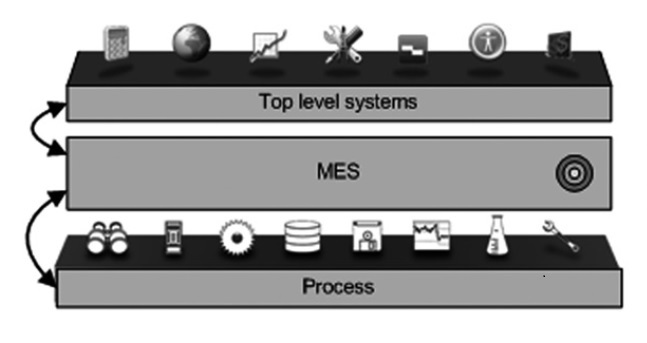
\includegraphics[width=.75\textwidth]{ch02/assets/mes_layers.jpg}
    \caption{Ambiente \glsfirst{mes} e as suas camadas, baseado em~\textcite[p.~526]{mes_literature_review}.}
    \label{fig:mes_layers}
\end{figure}

Com o intuito de dar resposta às necessidades de diversos ambientes produtivos, as funções apresentadas na Figura~\ref{fig:mes_functions} e descriminadas a seguir são essenciais para um \gls{mes}, nomeadamente no suporte, no controlo e na rastreabilidade de cada atividade produtiva~\parencite{mes_literature_review, mes_explained_high_level_vision, introduction_mes}:

\begin{enumerate}
    \item 
    {
        \textit{Operações/Agendamento de detalhes} -- sequenciamento e distribuição temporal das atividades fabris, por forma a otimizar a \textit{performance}, com base nos recursos disponíveis;
    }
    \item
    {
        \textit{Gestão do processo} -- controlo do fluxo de trabalho, baseado nas atividades produtivas reais e planeadas;
    }
    \item
    {
        \textit{Controlo documental} -- gestão e distribuição de informação relativa a produtos, processos, ordens de fabrico, assim como recolher os certificados e condições de trabalho;
    }
    \item
    {
        \textit{Aquisição de dados} -- monitorização, recolha e tratamento de dados sobre os processos, os materiais e operações, por pessoas, máquinas ou controlos;
    }
    \item
    {
        \textit{Gestão laboral} -- supervisão no uso de pessoal de operações num determinado turno, com base nas qualificações, padrões de trabalho e na necessidade de negócio;
    }
    \item
    {
        \textit{Gestão da qualidade} -- registo e análise das características do produto e do processo face aos requisitos ideais;
    }
    \item
    {
        \textit{Expedição de unidades de produção} -- dar a ordem para envio de materiais ou ordens para certos setores da fábrica, com o intuito de iniciar um processo ou sub-processo;
    }
    \item
    {
        \textit{Gestão de manutenção} -- planeamento e execução de tarefas que visam manter o equipamento e outros ativos capazes de executar a sua tarefa, de forma eficaz;
    }
    \item
    {
        \textit{Genealogia e rastreabilidade do produto} -- monitorização do progresso das unidades, amostras ou lotes de saída, para a criação de histórico completo do produto;
    }
    \item
    {
        \textit{Análise de desempenho} -- comparação dos resultados medidos com os objetivos e métricas definidas pela corporação, pelos clientes ou órgãos reguladores;
    }
    \item
    {
        \textit{Estado e alocação de recursos} -- orientação sobre o que as pessoas, máquinas ou ferramentas devem fazer, acompanhando que já fizeram e o que estão a fazer no momento.
    }
\end{enumerate}

\begin{figure}[!ht]
    \centering
    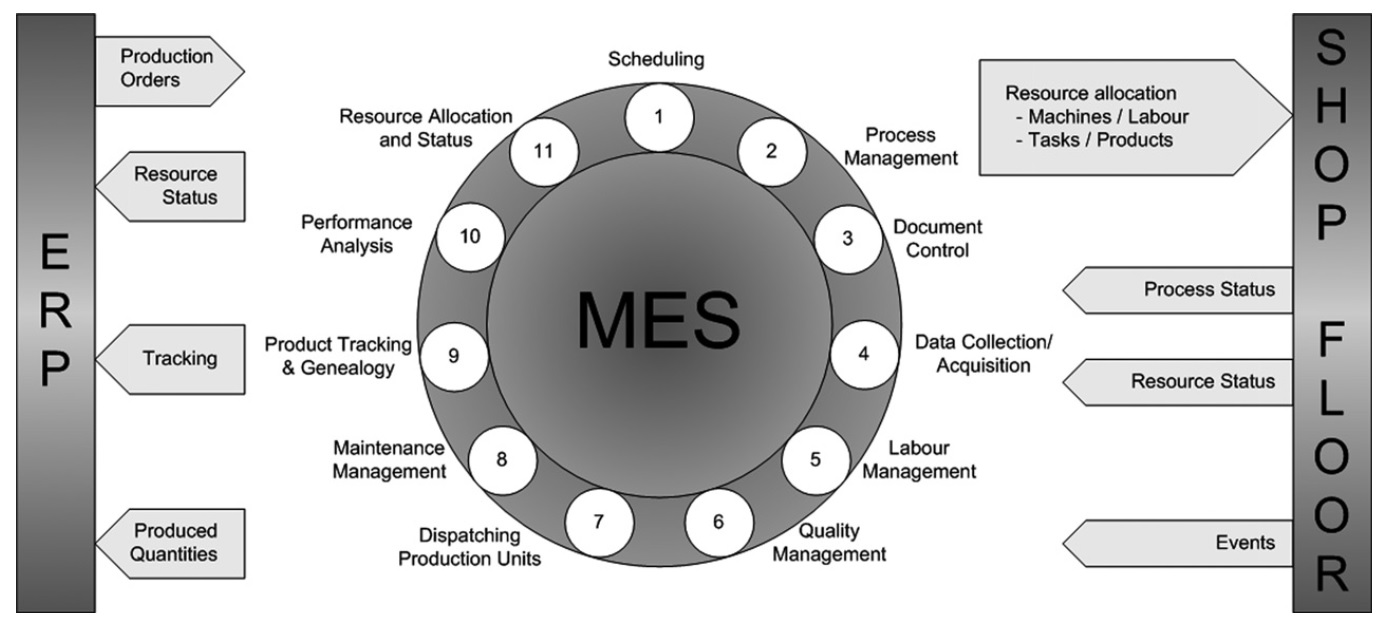
\includegraphics[width=.9\textwidth]{ch02/assets/mes_functions.jpg}
    \caption{Funções do \glsfirst{mes} e o seu enquadramento, extraído de~\textcite{mes_literature_review}}
    \label{fig:mes_functions}
\end{figure}

As funções do \gls{mes} enunciadas servem como base para praticamente qualquer fábrica, fornecendo ferramentas a gestores de fábrica, departamentos de qualidade e manutenção, estando interrelacionadas. Por isso, tratam-se de funções críticas para a maioria dos fabricantes, na medida em que a exigência de processos novos e mais rigorosos no negócio é viável, possibilitando o sucesso no mercado~\parencite{,mes_explained_high_level_vision}. Logo, torna-se evidente que o \gls{mes} traz benefícios para as corporações, alguns alcançáveis num período curto de tempo -- aumento de eficiência e redução de custos; redução no tempo de execução de ordens de fabrico; redução dos custos associados ao trabalho; diminuição ou eliminação de papelada; redução da quantidade de material em processamento; utilização de máquinas mais eficaz --, enquanto que outros, possíveis a longo prazo -- melhoria geral dos processos; maior satisfação do cliente; melhoria na conformidade regulamentar; maior agilidade; melhoria nos prazos de entrega; maior visibilidade da cadeia logística~\parencite{cmf_mes_definition}.

\subsection{{\productname}}

O {\productname} afirma-se como o futuro do \gls{mes}. Trata-se de uma plataforma de \textit{software} inovadora, com um vasto conjunto modular de aplicações e ferramentas, que dotam os utilizadores de indústrias complexas de agilidade, visibilidade e fiabilidade. O produto adapta-se a diversos processos fabris e às suas operações, sendo fácil a sua implantação, independentemente da infraestrutura existente, permitindo o controlo de produção e de custos na empresa e cadeia logística, resultando nas seguintes vantagens~\parencite{cmf_product_overview}:

\begin{enumerate}
    \item 
    {
        Apresenta um \textbf{baixo custo total de posse}\footnote{\textit{Total Cost of Ownership} (TCO). É uma estimativa financeira usada para avaliar os custos diretos e indiretos associados a uma compra.}, visto que a empresa reduz as despesas associadas à implantação, operação e manutenção do sistema;
    }
    \item
    {
        Fornece um largo conjunto de capacidades que dão resposta aos mais variados requisitos, demonstrando a sua \textbf{cobertura funcional};
    }
    \item
    {
        \textbf{Capacita o utilizador na sua função}, sendo este capaz de desenhar e colocar em produtivo o plano da fábrica, rastreando os materiais e os detalhes do processo;
    }
    \item
    {
        É sistema modular, o que o torna \textbf{extensível, flexível e escalável}, dando aos seus utilizadores acesso a inteligência operacional, de forma fácil e rápida; 
    }
    \item
    {
        A arquitetura logicamente descentralizada, ligada à conectividade a diferentes protocolos para equipamentos e dispositivos e ao suporte de produtos preparados para \gls{iot} e \glspl{cps}, tornam o produto \textbf{preparado para a Indústria 4.0}.
    }
\end{enumerate}

Relativamente à arquitetura do produto, demonstrada na Figura~\ref{fig:mes_framework}, a {\companyname} baseou-se nas tecnologias mais
recentes para dotar a sua plataforma da capacidade de adaptação aos diversos ambientes produtivos. Posto isto, a infraestrutura consiste em três camadas, que além de fornecerem particionamento, modularidade e escalabilidade das aplicações, foram projetadas para funcionar em conjunto. Além disso, esta foi desenhada de forma a ser customizável e extensível, dado que cada cliente pode ter os seus próprios requisitos~\parencite{cmf_mes_framework}.

\begin{figure}[!ht]
    \centering
    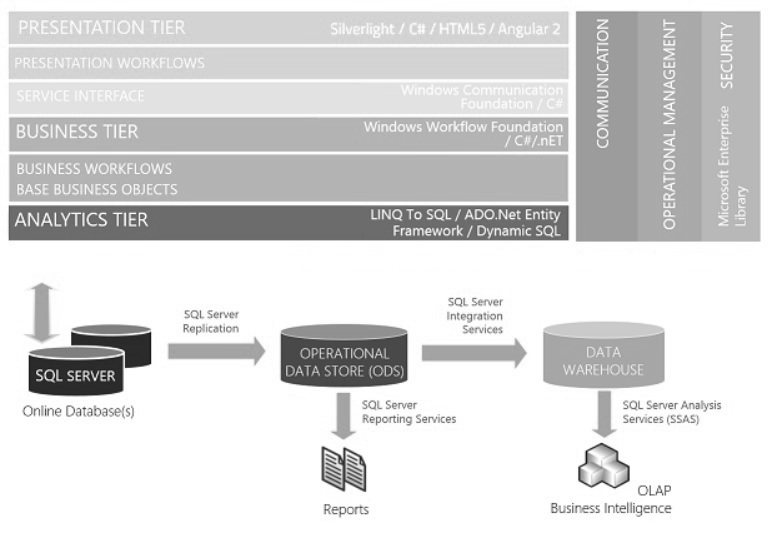
\includegraphics[width=.9\textwidth]{ch02/assets/mes_framework.jpg}
    \caption{Arquitetura do {\productname} e tecnologias usadas, baseado em~\textcite{cmf_mes_framework}}
    \label{fig:mes_framework}
\end{figure}

Quanto às especificidades de cada camada, são descritas de seguida, numa perspetiva de entender a responsabilidade de cada uma delas e o seu contributo para a plataforma~\parencite{cmf_mes_framework}. Já as tecnologias usadas estão especificadas na Figura~\ref{fig:mes_framework}.

\begin{itemize}
    \item 
    {
        \textit{Camada de Apresentação (Presentation Tier)} -- projetada para trazer ao utilizador uma experiência rica e interativa. Dispõe de várias capacidades (\exempligratia{permitir aos utilizadores criar a sua própria interface gráfica ou desenvolver ecrãs para um propósito em particular, numa fábrica ou setor}) e é desenvolvida com suporte multi-plataforma, executando em qualquer sistema operativo \textit{desktop} ou móvel;
    }
    \item
    {
        \textit{Camada de Negócio (Business Tier)} -- implementa e expõe todas as funcionalidades como serviços, estando disponíveis vários protocolos de comunicação. Contém uma sub-camada de orquestração usada para definir os diversos fluxos de negócio, fornecendo a capacidade de coordenação usando os objetos de negócio. Por fim, a sub-camada de objetos de negócio segue um modelo hierárquico, o qual facilita o desenvolvimento de entidades com um comportamento comum;
    }
    \item
    {
        \textit{Camada de Dados (Data Tier)} -- desenhado para suportar as capacidades de armazenamento de dados, possibilitando a integração com fontes de dados externas, geração e modificação de relatórios e mineração de dados.
    }
\end{itemize}

O {\productname} é usado em diversas indústrias, particularmente a indústria de semicondutores~\parencite{cmf_industries_semiconductor}, de equipamentos médicos~\parencite{cmf_industries_medical_devices}, de montagem eletrónica~\parencite{cmf_industries_electronics}, procurando dar resposta aos desafios inerentes a cada uma delas.


% Análise de Valor
\section{Análise de Valor}
\label{sec:chap02_valueanalysis}

Até ao momento, deu-se o contexto do trabalho a ser desenvolvido, de forma a perceber a realidade atual dos sistemas de controlo de produção. Contudo, é preciso perceber qual o impacto que a solução a ser desenvolvida terá no produto e no mercado no qual se insere. Visto que o módulo a desenvolver será integrado num produto já existente, analisa-se a oportunidade de negócio que surge com a nova funcionalidade.

\subsection{O Processo de Inovação}

De acordo com~\textcite{ffe_effectivemethods_tools_techniques}, o processo de inovação, representado na Figura~\ref{fig:inovation_process}, está dividido em três áreas -- o \gls{ffe}, \gls{npd} e a comercialização -- que correspondem às fases inerentes ao \gls{ncd}, um modelo desenvolvido por um conjunto de empresas, com o objetivo de \inquotes{[...]~fornecer uma linguagem e compreensão comum para as atividades \textit{front end}}\footnote{Tradução livre de autor. No original \inquotes{[...]~to provide a common language and insights on the front end activities.}.}~\parencite{providing_clarity_common_language_ffe}.

O \gls{ffe} representa uma oportunidade para melhoria de todo o processo de inovação, focando todas as atividades que antecedem o desenvolvimento do produto, com o propósito de potenciar o valor, a importância e a probabilidade de sucesso das fases que se seguem. Ou seja, consiste no investimento do tempo em atividades de discussão da ideia, por forma a identificar e estruturar o problema ou oportunidade~\parencite{ffe_effectivemethods_tools_techniques, ffe_theoretical_model}. Porém, as atividades inerentes ao \gls{ffe} são fundamentalmente diferentes da fase \gls{npd}, pelo que se torna necessária a definição de vocabulário específico, permitindo a geração de conhecimento e clara distinção entre as diferentes fases do processo~\parencite{ffe_effectivemethods_tools_techniques}.

\begin{figure}[!ht]
    \centering
    \includegraphics[width=.95\textwidth]{ch02/assets/inovation_process.jpg}
    \caption{O processo de inovação, extraído de~\textcite{ffe_effectivemethods_tools_techniques}}
    \label{fig:inovation_process}
\end{figure}

O modelo \gls{ncd}, demonstrado na Figura~\ref{fig:ncd_model}, baseado num modelo relacional ao invés de um processo linear, visa providenciar uma terminologia para o \gls{ffe}~\parencite{ffe_effectivemethods_tools_techniques}. A área interna define os cinco elementos chave do \textit{Front End of Inovation}: a identificação de oportunidade (\textit{Opportunity Identification}), a análise de oportunidade (\textit{Opportunity Analysis}), a geração e enriquecimento de ideias (\textit{Idea Generation and Enrichment}), a seleção de ideias (\textit{Idea Selection}) e a definição do conceito (\textit{Concept Definition}). O motor central (\textit{Engine}) corresponde à liderança, cultura e estratégia organizacional, que suporta os elementos que compõem o \gls{ffe}, são controláveis pela organização e possibilita a interação entre eles. Já na periferia, encontram-se os fatores de influência (\textit{Influencing Factors}), geralmente incontroláveis pela organização, consistem nas capacidades organizacionais, na estratégia de negócio, no mundo exterior, nomeadamente os canais de distribuição, clientes, fornecedores, concorrentes, política governamental ou legislação, ou quaisquer fatores que possam influenciar todo o processo de inovação~\parencite{ffe_effectivemethods_tools_techniques, providing_clarity_common_language_ffe}.

\begin{figure}[!ht]
    \centering
    \includegraphics[width=.55\textwidth]{ch02/assets/ncd_model.jpg}
    \caption{A representação do modelo \glsfirst{ncd}, extraído de~\textcite{ffe_effectivemethods_tools_techniques}}
    \label{fig:ncd_model}
\end{figure}

Quanto à representação do modelo, as partes internas são designadas de elementos por oposição a processos, pois estes implicam estrutura, que pode não ser possível ser aplicada. O formato circular indica que é esperado que as ideias fluam, circulem e iterem ao longo dos elementos, por qualquer ordem ou combinação, permitindo o uso dos elementos, repetidamente. Este comportamento é intrínseco às atividades do \gls{ffe}, permitindo uma definição clara do mercado, dos requisitos, dos riscos associados e do plano de negócio, tornando mais eficazes as fases de desenvolvimento e comercialização, devido à redução do tempo total de projeto, fruto da diminuição da repetição de algumas atividades~\parencite{ffe_effectivemethods_tools_techniques}. 

\subsection{O \textit{Fuzzy Front End} de Inovação}

Como mencionado anteriormente, o \gls{ffe} corresponde a um conjunto de atividades geralmente caóticas, imprevisíveis e não estruturadas que antecedem o desenvolvimento de um produto~\parencite{ffe_incremental_platform_breakthrough_products}. Todavia, é preciso perceber a natureza do produto a desenvolver, de forma a melhor enquadrar o processo de inovação.

Segundo~\textcite{ffe_incremental_platform_breakthrough_products}, pode-se caracterizar os produtos de acordo com a extensão da mudança ou do processo: incremental, requer pouca mudança a nível do produto ou do processo, uma vez que geralmente consiste na redução de custos, melhoria, extensão ou reposicionamento no mercado de produtos já existentes; plataforma, estabelecem uma arquitetura básica para uma nova geração de produtos ou processos; pioneiro, envolve uma mudança significativa no processo ou produto.

O presente trabalho visa o desenvolvimento dum módulo de linguagem natural para o {\productname}, uma plataforma já estabelecida, ou seja, trata-se de uma extensão ao produto já existente, enquadrando-se no tipo incremental. A ideia surge do processo de planeamento estratégico da empresa com a finalidade de trazer novas funcionalidades aos seus clientes, melhorando a qualidade do produto. Portanto, nas secções seguintes, aplica-se a metodologia explicitada, no sentido de enriquecer a proposta de projeto apresentada pela {\companyname}.

\subsubsection{Identificação da Oportunidade}

O \gls{pln} é uma área de investigação que explora a forma como os computadores podem manipular a linguagem natural (texto ou voz) para executar determinadas tarefas. Aplica-se em diversos campos de estudo: tradução, processamento de texto, interfaces com o utilizador, reconhecimento de voz, sistemas periciais~\parencite{nlp}.

\textcite{end_to_end_neural_nli_databases} menciona que, apesar da expressividade da \gls{sql}, os utilizadores necessitam de algum conhecimento técnico para perceber como extrair informação de um sistema, o que conduziu à investigação para o desenvolvimento de interfaces alternativas que permitam aos utilizadores, sem conhecimento técnico, explorar e interagir com os dados, de forma conveniente. Também \textcite{towards_theory_nli_databases} menciona que a necessidade de interfaces de linguagem natural se torna mais evidente, devido ao número de pessoas sem conhecimentos técnicos que acedem a informação através de \textit{browsers} ou telemóveis, tornando paradigmas como o reconhecimento de voz mais atrativos.

Nesse sentido, a {\companyname} tenciona o desenvolvimento do módulo de linguagem natural para que os utilizadores do produto, sem conhecimento orientado às tecnologias de informação, possam fácil, rápida e intuitivamente consultar o sistema. Desta forma, a funcionalidade destaca o produto pelo uso de novas tecnologias, facilita-se a interação com o sistema, reduzindo-se o tempo de formação técnica associado ao mesmo. 

\subsubsection{Análise da Oportunidade}

A pesquisa realizada por~\textcite{roadmap_nlp_research_is}, apresentada na Figura~\ref{fig:number_articles_per_year_nlp}, cuja metodologia consistiu na pesquisa de termos como \inquotes{Natural Language Processing} e \inquotes{NLP} em bases de dados académicas, determina que tem havido uma tendência crescente de interesse por esta área. Nos últimos anos, a quantidade de dados textuais disponíveis nas redes sociais ou em sistemas de comunicação, juntamente com a necessidade de acesso a informação, contribuíram para o avanço e adoção comercial do \gls{pln}~\parencite{roadmap_nlp_research_is}.

\begin{figure}[!ht]
    \centering
    \includegraphics[width=.9\textwidth]{ch02/assets/number_articles_nlp.jpg}
    \caption{Número de artigos de \glsfirst{pln} pesquisados por ano, extraído de~\textcite{roadmap_nlp_research_is}}
    \label{fig:number_articles_per_year_nlp}
\end{figure}

Quanto ao segmento de mercado no qual se integra, cresce a visão de fábricas inteligentes, associadas à quarta revolução industrial, prezando a integração do operador humano num ambiente complexo e rico em dados~\parencite{social_factory}. \textcite{industry40_revolution_future_mes} afirma que a revolução supracitada é já conhecida pelas empresas, o que lhe permite tomar ações no sentido de definir o seu modelo de fabrico e o seu plano de transformação, particularmente na adaptação do \gls{mes} de forma a manter o desempenho, qualidade e agilidade nas desafios espoletados pelas empresas de manufatura. Portanto, a interação entre o ser humano e o sistema pode melhorar o processo de fabrico e potenciar o negócio, na medida em que o operador, em vez do trabalho manual repetitivo que pode facilmente ser automatizado, passa a tomar decisões no processo para resolução de problemas, as quais requerem acesso à informação correta e de forma atempada~\parencite{social_factory}. É nesse sentido que o {\productname} ganha vantagem com o desenvolvimento desta nova funcionalidade.

\subsubsection{Geração, Enriquecimento e Seleção de Ideias}

No seguimento deste assunto, foram realizadas duas reuniões com o supervisor do projeto na {\companyname}, em que foram discutidos alguns requisitos operacionais e de usabilidade, restrições ao desenvolvimento da solução, como a preferência por uso de ferramentas de \gls{pln} que possam ser mantidas internamente e a sua facilidade de utilização, e ideias para futuras implementações, as quais podem ter um impacto na especificação arquitetural do protótipo.

\begin{figure}
    \centering
    \resizebox{\textwidth}{!}{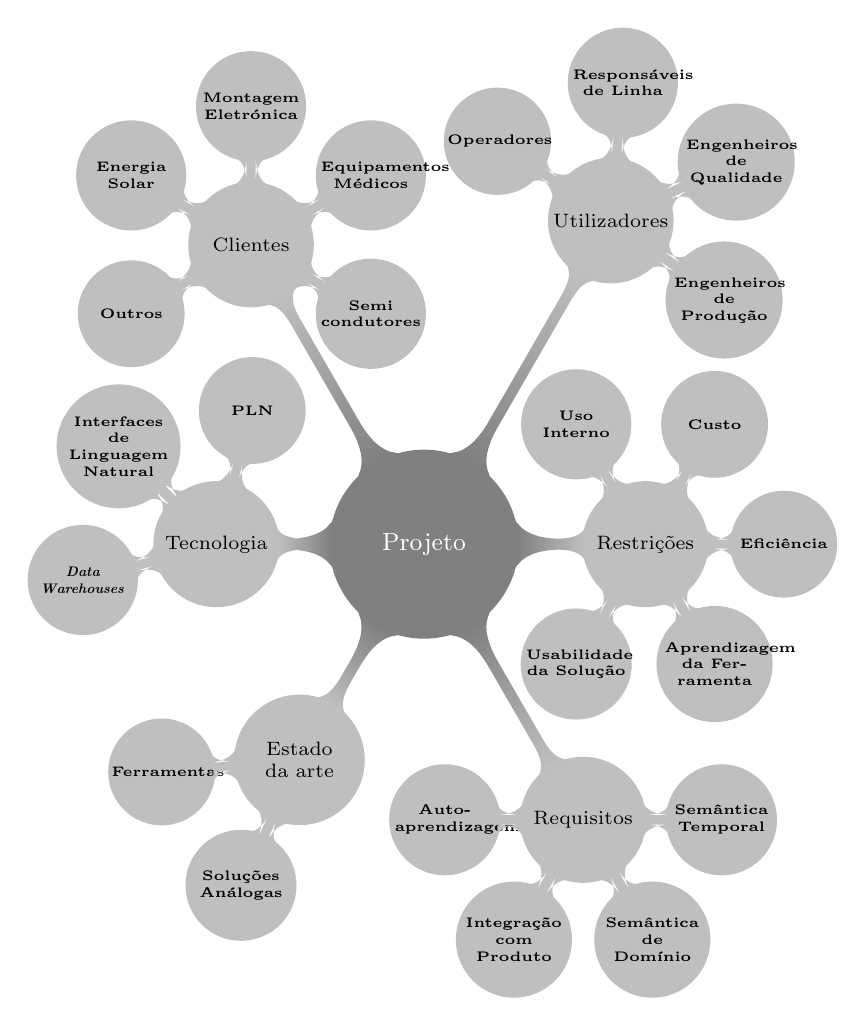
\begin{tikzpicture}
  \path[mindmap, concept color=black!50,text=white,
    every node/.append style={concept, minimum size=0.5cm, inner sep=0.2mm},
    level 1 concept/.append style={text width=1.5cm,font=\scriptsize},
    level 2 concept/.append style={text width=1.27cm,font=\tiny\bfseries,level distance=50}
  ]
    % Root
    node[text width=2.3cm,font=\small] {Projeto}
    %
    [clockwise from=0]
    child[concept color=black!25,text=black,level distance=80] { node {Restrições}
      [clockwise from=120]
      child { node {Uso Interno} }
      child { node {Custo} }
      child { node {Eficiência} }
      child { node {Aprendizagem da Ferramenta} }
      child { node {Usabilidade da Solução} }
    }
    %
    child[concept color=black!25,text=black,level distance=115] { node {Requisitos}
      [clockwise from=0]
      child { node {Semântica Temporal} }
      child { node {Semântica de Domínio} }
      child { node {Integração com Produto} }
      child { node {Auto-aprendizagem} }
    }
    %
    child[concept color=black!25,text=black,level distance=90] { node {Estado da arte} 
      [clockwise from=-115]
      child { node {Soluções Análogas} }
      child { node {Ferramentas} }
    }
    %
    child[concept color=black!25,text=black,level distance=75] { node {Tecnologia}
      [counterclockwise from=75]
      child { node {PLN} }
      child { node {Interfaces de Linguagem Natural} }
      child { node {\textit{Data Warehouses}} }
    }
    %
    child[concept color=black!25,text=black,level distance=125] { node {Clientes}
      [counterclockwise from=-30]
      child { node {Semi\\condutores} }
      child { node {Equipamentos Médicos} }
      child { node {Montagem Eletrónica} }
      child { node {Energia Solar} }
      child { node {Outros} }
    }
    child[concept color=black!25,text=black,level distance=135] { node {Utilizadores}
      [counterclockwise from=-35]
      child { node {Engenheiros de Produção} }
      child { node {Engenheiros de Qualidade} }
      child { node {Responsáveis de Linha} }
      child { node {Operadores} }
    };
\end{tikzpicture}}
    \caption{\textit{Mindmap} das ideias e conceitos gerados}
    \label{fig:mindmap}
\end{figure}

Em relação às ideias e conceitos contempladas no \textit{mindmap} da Figura~\ref{fig:mindmap}, o presente projeto pretende dar resposta a praticamente todos, tendo em consideração que, numa fase inicial, o cumprimento de todos é praticamente inatingível. A descrição de cada conceito é feito de seguida:

\begin{itemize}
    \item
    {
        \textit{Tecnologia} -- a ideia inerente ao trabalho assenta sobre as temáticas de \gls{pln}, especificamente Interfaces de Linguagem Natural, e \textit{Data Warehouses}. Esta consiste no estudo aprofundado deste tipo de interfaces orientado à consulta em armazéns de dados e disseminação do conhecimento internamente, para que no futuro, o projeto possa ter continuidade;
    }
    \item
    {
        \textit{Estado da Arte} -- abordagem de ferramentas e soluções análogas, com o objetivo de especificar uma arquitetura para o sistema. Este processo dá origem aos documentos de especificação que devem ser usados para consulta por parte dos desenvolvedores, quer numa perspetiva de conhecimento arquitetural, quer das ferramentas que são usadas;
    }
    \item
    {
        \textit{Clientes} -- uma vez que a {\companyname} possui clientes com diferentes realidades, a ideia é que o módulo final esteja preparado para elaborar consultas em qualquer domínio, de forma configurada ou cerne da solução. Contudo, como já abordado anteriormente, no contexto deste trabalho, apenas um domínio será considerado;
    }
    \item
    {
        \textit{Utilizadores} -- a solução deverá responder às necessidades de qualquer utilizador, desde os mais técnicos (Engenheiros de Produção) aos menos técnicos (Operadores). Porém, o protótipo terá em consideração os utilizadores mais comuns do {\productname};
    }
    \item
    {
        \textit{Restrições} -- nesta temática, foram discutidas alternativas de como avaliar o custo de uma ferramenta proprietária, uso de ferramentas \textit{Open Source} ou o desenvolvimento interno da própria biblioteca de \gls{pln}, para garantir que não existem dependências externas à plataforma, a eficiência da solução em contexto produtivo, a facilidade de aprendizagem e usabilidade da mesma. Assim, a usabilidade da solução será estudada a partir do mecanismo de \textit{feedback} provido no módulo e através de inquéritos aos utilizadores, o que também se aplica para a aprendizagem da ferramenta. Relativamente aos restantes tópicos, não houve conclusão acerca das ideias a serem selecionadas;
    }
    \item
    {
        \textit{Requisitos} -- pressupõe-se o uso de auto-aprendizagem para adaptação automática do módulo ao \textit{feedback} do utilizador, ainda que para o protótipo, a resposta a uma simples pergunta como \inquotes{A resposta obtida foi-lhe útil?} é suficiente. Também a integração com o produto, quer a nível aplicacional, quer a nível de processo deve ser considerada, o que resultará na organização de \textit{meetups} com as equipas responsáveis pelo processo de manutenção da plataforma. Quanto aos restantes conceitos, não houve conclusão acerca das ideias selecionadas.
    }
\end{itemize}

\subsubsection{Definição do Conceito}

Todo o processo presente no modelo \gls{ncd} de \gls{ffe} culmina com a definição do conceito, a fase que encaminha o projeto para a implementação~\parencite{ffe_effectivemethods_tools_techniques}.

O presente trabalho, denominado de \inquotes{Natural Language Querying} consiste no desenvolvimento de um módulo de linguagem natural para interface com o {\productname}. Este módulo permitirá a consulta e pesquisa de estados do processo de fabrico por utilizadores com pouco ou nenhum conhecimento associado a tecnologias de informação, garantindo a interação com o sistema de uma forma simples, fácil e intuitiva, melhorando o processo numa perspetiva de apoio à decisão (ver Secção~\ref{sec:chap01_problem}). Os objetivos deste projeto estão descritos na Secção~\ref{sec:chap01_objectives}, a metodologia e critérios de sucesso na Secção~\ref{sec:chap01_solutionevaluation}, e o respetivo plano de trabalho no Capítulo~\ref{sec:chap01_workmethodology}.

O projeto traz benefícios para a empresa e o seu produto, pela adoção de tecnologia de \gls{pln} num contexto industrial, pela melhoria de usabilidade do sistema e pela evolução no processo de apoio à decisão dos seus clientes. Uma vez que o {\productname} é um produto bem posicionado no mercado, não se esperam riscos a nível comercial. Contudo, a uso de tecnologia recente, cujos conceitos não estão totalmente estudados e cujos trabalhos de investigação são limitados, pode provocar atrasos no desenvolvimento do projeto ou incumprimento do orçamento definido. Não obstante, o projeto avança com o desenvolvimento de um protótipo, fase que decidirá a inclusão do módulo na plataforma da {\companyname}.


\chapter{Estado da Arte}
\label{chap:Chapter3}
O presente capítulo tem como objetivo apresentar os conceitos pertinentes para a execução e compreensão do trabalho, as ferramentas de \gls{pln} disponíveis no mercado, relevantes para a resolução do problema e os projetos que focam um problema de cariz semelhante. Na Secção~\ref{sec:chap03_pln} é introduzido o conceito de Processamento de Linguagem Natural, enquadrando-o com a solução a desenvolver. A Secção~\ref{sec:chap03_marketstudy} explora-se o mercado numa perspetiva de encontrar casos de estudo para a solução a desenvolver. Por fim, a Secção~\ref{sec:chap03_existingtools} discrimina as ferramentas mais significativas para a área \gls{pln} e em que medida é que cada uma pode, ou não, contribuir para o trabalho e a Secção~\ref{sec:chap03_approaches} distingue algumas abordagens postas em prática, com o objetivo de testar e avaliar, no ponto de vista de aplicabilidade, cada uma delas.

%%%%%%%%%%%%%%%%%%%%%%%%%%%%%%%%%
%           SECTION
%%%%%%%%%%%%%%%%%%%%%%%%%%%%%%%%%
\section{Processamento de Linguagem Natural}
\label{sec:chap03_pln}
O \glsfirst{pln} é um campo da Ciência da Computação, \glsfirst{ia} e Linguística que explora a forma como os computadores podem ser usados na compreensão, manipulação e geração automática da linguagem natural, em forma de texto ou voz~\parencite{nlp, applied_natural_language_processing_with_python, pln_extracao_conhecimento}. Nos últimos anos, a área tem-se tornado bastante popular com o acesso fácil a informação através da Internet, estando presente em implementações de \textit{chatbots}, verificadores ortográficos em telemóveis e assistentes de \gls{ia} nos \textit{smartphones}, tais como a Cortana\footnote{Disponível em \url{https://www.microsoft.com/en-us/cortana}.} ou Siri\footnote{Disponível em \url{https://www.apple.com/siri/}.}~\parencite{pln_extracao_conhecimento, applied_natural_language_processing_with_python}. 

\subsection{História}
O início do \gls{pln} remonta aos anos 40, com o desenvolvimento da Ciência da Computação, aliada aos avanços na Linguística, que levou ao aparecimento da teoria da linguagens formais. Muito sucintamente, esta teoria consiste na modelação de estruturas complexas e respetivas regras, ou seja, permitem especificar e reconhecer linguagens a partir de modelos matemáticos (\exempligratia{um alfabeto é uma estrutura simples, a qual é constituída por letras que podem formar palavras, em diferentes idiomas}). Por outro lado, os avanços na \gls{ia}, particularmente com o modelo \gls{slp} apresentado na Figura~\ref{fig:slp}, também contribuíram para este campo~\parencite{applied_natural_language_processing_with_python}. O \gls{slp} é a base dos modelos neuronais usados nos dias de hoje. Warren McCulloch e Walter Pitts propuseram este modelo, baseado na analogia entre células nervosas (neurónios) e os processos computacionais, que permite computar a soma dos pesos ($w_{ni}$) associados a cada entrada ($x_{n}$), dando uma resposta binária consoante o valor da soma ($\sum$) varia de acordo com um determinado valor limite, decidindo se uma determinada ação será executada~\parencite{introduction_theory_neural_computation}.

\begin{figure}[!t]
    \centering
    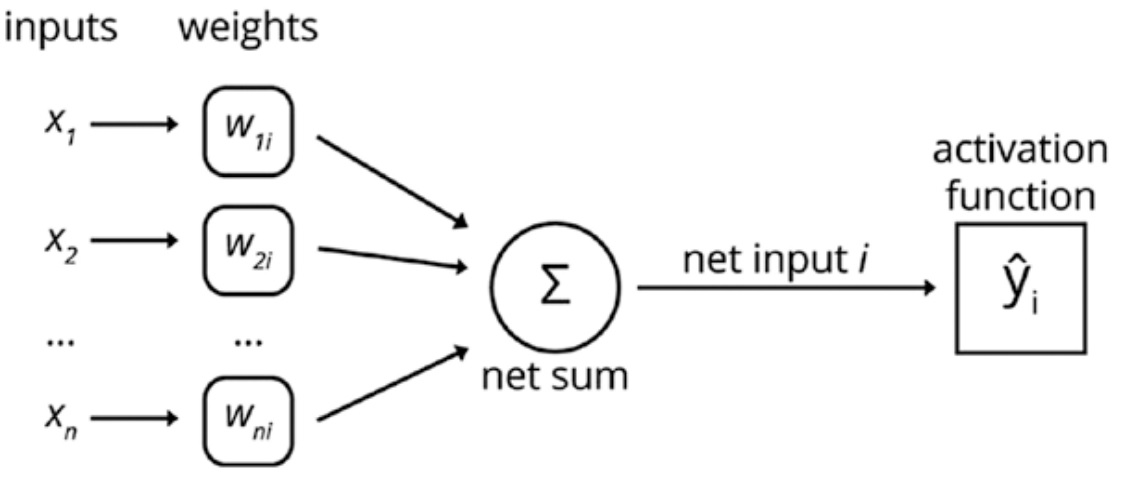
\includegraphics[width=.8\textwidth]{ch03/assets/slp_model.jpg}
    \caption{\glsfirst{slp}, extraído de~\textcite{applied_natural_language_processing_with_python}}
    \label{fig:slp}
\end{figure}

Ao longo dos anos, várias técnicas foram surgindo na tentativa de resolver problemas associados à compreensão da linguagem natural. Mas, nos últimos 20 anos, notou-se o aumento de interesse no \gls{pln}, juntamente com \gls{ml}, sobretudo devido ao aumento do poder computacional e à facilidade de acesso a dados etiquetados através da Internet~\parencite{applied_natural_language_processing_with_python}.

\subsection{Fundamentos}
O cerne de qualquer tarefa de \gls{pln} está relacionado com a compreensão da própria linguagem. O desenvolvimento deste tipo de aplicações incorre em alguns problemas tais como a processo de pensamento, a representação e significado linguístico e/ou conhecimento do domínio, que estão associados à ambiguidade da linguagem natural~\parencite{nlp, pln_extracao_conhecimento}. Por outras palavras, a ambiguidade surge quando não é possível atribuir um significado único a uma dada expressão. Se uma pessoa é capaz de o fazer, baseada na sua experiência, capacidade de interpretação de contexto ou na sua cultura, já um computador não tem essa mesma capacidade~\parencite{pln_extracao_conhecimento}. Por isso, \textcite{nlp} enuncia que, para ser capaz de compreender a linguagem natural, é importante considerar os vários níveis de conhecimento interdependentes que o ser humano usa na extração de significado:

\begin{itemize}
    \item 
    {
        \textit{Nível fonético ou fonológico} -- encarrega-se a pronúncia;
    }
    \item
    {
        \textit{Nível morfológico} -- lida com os \textit{tokens}, ou seja, partes nucleares de um frase (\exempligratia{palavras, sufixos, prefixos, sinais de pontuação, dígitos, entre outros});
    }
    \item
    {
        \textit{Nível léxico} -- trata do significado léxico dos símbolos e análise de partes do discurso;
    }
    \item 
    {
        \textit{Nível sintático} -- lida com a gramática e a estrutura frásica;
    }
    \item
    {
        \textit{Nível semântico} -- encarrega-se de clarificar o significado da frase ou das palavras;
    }
    \item
    {
        \textit{Nível pragmático} -- ocupa-se da relação entre a linguagem e o contexto, ou seja, contempla a relação com o mundo exterior;
    }
    \item
    {
        \textit{Nível de discurso} -- suporta o agrupamento de diferentes frases, identificando a relação entre elas, de forma a compreender o contexto.
    }
\end{itemize}

Um sistema \gls{pln} pode envolver todos ou alguns destes níveis, cujas atividades permitem solucionar pequenas partes de um problema mais complexo. Algumas destas tarefas ou ferramentas incluem técnicas de segmentação de palavras e construção frásica, \textit{parsing} sintático e estatístico, métodos de desenho de modelos de conhecimento estruturados, redes neuronais e modelos de linguagem neuronal~\parencite{nlp, speech_language_processing}.

\subsection{Interfaces de Linguagem Natural}
Uma interface de linguagem natural é um componente que aceita expressões de consulta ou comandos em linguagem natural e providencia as respostas apropriadas, ou seja, esta deve ser capaz de traduzir as frases nas respetivas ações para o sistema~\parencite{nlp}. Neste contexto particular, importa explorar as \gls{ilnbd}, as quais permitem os utilizadores executarem pesquisas em bases de dados usando a linguagem natural~\parencite{overview_nlidb_approaches_implementation_airline, novel_approach_building_generic_portable_contextual_nlidb_system}.

As \gls{ilnbd} apresentam um problema clássico na área de \gls{pln} e constitui um campo de estudo em desenvolvimento. Genericamente, a solução inerente a este problema podem ser divida em duas fases: processamento linguístico, em que a frase de pesquisa é mapeada e traduzida para a \textit{query} de \gls{sql} correspondente, usando funções de mapeamento adequadas; processamento na base de dados, na qual é executado a gestão de acesso ao sistema e execução da respetiva consulta~\parencite{overview_nlidb_approaches_implementation_airline}. Este tipo de sistemas é capaz de responder a uma grande variedade de \textit{queries} de linguagem natural mas são pouco usados comercialmente, principalmente pela pouca robustez nas capacidades de processamento de contexto~\parencite{novel_approach_towards_incorporating_context_processing_nlidb}, pela falta de cobertura linguística ou pelo facto de utilizador poder assumir inteligência por parte do sistema~\parencite{survey_nlidb, overview_nlidb_approaches_implementation_airline}. Ainda assim, existem várias vantagens que contribuem para o desenvolvimento deste tipo de aplicações, nomeadamente a facilidade e simplicidade de utilização, o facto de ser mais adequado para questões que envolvem negação ou quantificação ou a sua tolerância a erros gramaticais~\parencite{survey_nlidb, nlidb_brief_review, overview_nlidb_approaches_implementation_airline}.

\begin{figure}[!h]
    \centering
    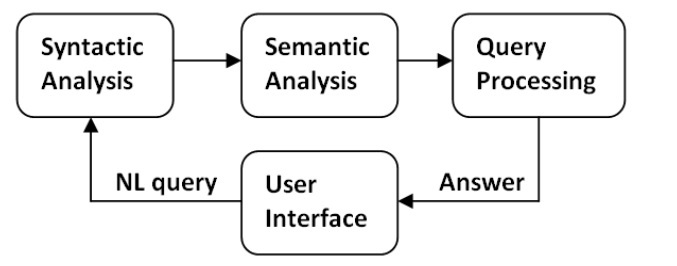
\includegraphics[width=.6\textwidth]{ch03/assets/non_contextual_nlidb.jpg}
    \caption{Sistema \glsfirst{ilnbd} não-contextual, extraído de~\textcite{novel_approach_towards_incorporating_context_processing_nlidb}}
    \label{fig:noncontextual_nlidb}
\end{figure}

Num ponto de vista processual, \textcite{novel_approach_towards_incorporating_context_processing_nlidb} menciona que os sistemas \gls{ilnbd} podem ser divididos em dois tipos: não-contextuais e contextuais. Num sistema não-contextual (Figura~\ref{fig:noncontextual_nlidb}) existe a necessidade de modelo semânticos de base, descrevendo regras de domínio. Na fase de análise sintática (\textit{Syntactic Analysis}) é extraída a informação linguística da \textit{query} de linguagem natural. Por sua vez, na análise semântica (\textit{Semantic Analysis}) identificam-se as entidades, atributos a partir da resposta da fase anterior e dos modelos semânticos. Finalmente, na fase de processamento de \textit{queries} (\textit{Query Processing}, as entidades identificadas são mapeadas num grafo, computando-se o caminho mais curto. Dessa forma, é gerada a \textit{query} \gls{sql} e executada para obter os resultados~\parencite{novel_approach_towards_incorporating_context_processing_nlidb}. Já um sistema \gls{ilnbd} contextual (Figura~\ref{fig:contextual_nlidb}) recolhe informação acerca do contexto numa \inquotes{conversa} com o utilizador. Neste caso, as capacidades de processamento devem ser contidas na arquitetura através da inserção de uma nova etapa (\textit{Context Processing}), mantendo intactas as responsabilidades de cada fase~\parencite{novel_approach_towards_incorporating_context_processing_nlidb}.

\begin{figure}[!h]
    \centering
    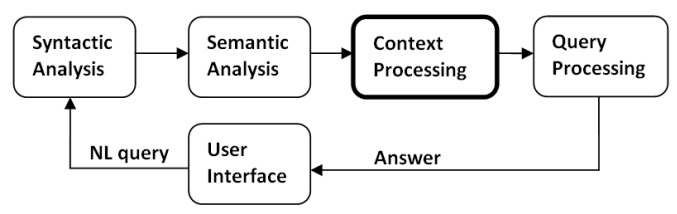
\includegraphics[width=.7\textwidth]{ch03/assets/contextual_nlidb.jpg}
    \caption{Sistema \glsfirst{ilnbd} contextual, extraído de~\textcite{novel_approach_towards_incorporating_context_processing_nlidb}}
    \label{fig:contextual_nlidb}
\end{figure}

Relativamente às abordagens ou estratégias de desenvolvimento deste tipo de \textit{software}, são várias e cada uma delas apresentam particularidades que podem influenciar a forma como o sistema é desenhado~\parencite{nlidb_brief_review, survey_nlidb}:

\begin{itemize}
    \item 
    {
        \textit{Abordagem simbólica (baseada em regras)} -- a linguagem é analisada e é aplicada lógica baseada em regras, de forma a capturar o significado da linguagem. O conhecimento encontra-se mapeado em regras ou noutras formas de representação;
    }
    \item
    {
        \textit{Abordagem empírica (baseada em experiências}) -- aplica análise estatística ou outro tipo de análises orientadas aos dados. Maior parte dos métodos de \gls{pln} aplicam técnicas estatísticas com modelos \textit{n-gram}, \textit{Hidden Markov} ou gramáticas de contexto livre;
    }
    \item
    {
        \textit{Abordagem de conexão (baseado em redes neuronais)} -- baseada em representações distribuídas que correspondem a regularidades estatísticas na linguagem. Uma vez que as capacidades da linguagem humana assentam na rede neuronal no cérebro, as redes neuronais artificiais apresentam um ponto fulcral na modelação do processamento de linguagem.
    }
\end{itemize}

Quanto à arquitetura dos sistemas \gls{ilnbd}, além de serem variadas, possuem também diferentes interpretações ao problema. Cada uma apresenta vantagens e desvantagens, pelo que é necessário explorar, de forma resumida, as características de cada.

\subsubsection*{Sistemas \textit{Pattern Matching}}
Os primeiros esforços no desenvolvimento de sistemas deste género começaram em meados do século XX. O conceito de \textit{Pattern Matching} permite mapear diretamente o \textit{input} do utilizador para a obter o resultado desejado. A implementação destes sistemas implica que os detalhes da base de dados estejam presentes no código, ou seja, torna a solução limitada a um contexto específico e ao número e complexidade de padrões existentes~\parencite{nlidb_brief_review}. A principal vantagem desta abordagem prende-se à simplicidade de implementação, pelo que não há necessidade em conceber módulos de interpretação ou \textit{parsing} da linguagem~\parencite{nlidb_brief_review, survey_nlidb}.

\subsubsection*{Sistemas Baseados em Sintaxe}
Os sistemas baseados em sintaxe possibilitam que a \inquotes{questão} do utilizador seja analisada sintaticamente, dando origem a uma árvore que é diretamente mapeada para uma expressão \gls{sql}. Para isso, estes sistemas usam uma gramática que descreve as estruturas sintáticas das perguntas dos utilizadores~\parencite{nlidb_brief_review}. Geralmente, é difícil mapear todas regras que constituem a gramática e o processo de escolha de quais as regras devem ser representadas é complexo. Outro problema é o facto de uma frase poder ter múltiplas corretas árvores de análise sintática, que aquando traduzidas, podem levar a diferentes resultados. Também a dificuldade de transformar a árvore de análise sintática diretamente numa linguagem genérica de base de dados é um problema complexo de resolver~\parencite{survey_nlidb}. A principal vantagem desta abordagem é o facto de fornecer informação acerca da estrutura frásica, possibilitando o mapeamento da semântica em regras produtivas (nós da árvore de análise sintática)~\parencite{nlidb_brief_review}.

\subsubsection*{Sistemas de Gramática Semântica}
Apesar da sua semelhança com os sistemas baseados em sintaxe, a ideia inerente a um sistema deste tipo é a simplificar a árvore de análise sintática, através da combinação de alguns nós ou remoção dos mesmos. Posto isto, um sistema de gramática semântica é capaz de refletir melhor a representação semântica da frase, sem as estruturas complexas na árvore, com a possibilidade de designar nomes para os nós, reduzindo a ambiguidade. As principais desvantagens desta abordagem prendem-se com a necessidade de conhecimento prévio do domínio, tornando-se difícil a transposição para um outro e a estrutura específica das árvores de análise sintática não poderia ser usado noutra aplicação~\parencite{survey_nlidb, nlidb_brief_review}.

\subsubsection*{Sistemas de Representação Intermediária de Linguagem}
Atualmente, os sistemas \gls{ilnbd} transformam a linguagem natural numa representação intermediária, definida internamente. Assim, a \textit{query} lógica representada na linguagem intermédia expressa o significado da questão colocada pelo utilizador em termos dos conceitos do domínio, os quais são independentes da estrutura da base de dados. Posteriormente, a \textit{query} lógica é traduzida na linguagem genérica de base de dados e avaliada. Esta arquitetura surgiu da dificuldade de traduzir diretamente a linguagem natural para a \gls{sql}, ou outra semelhante. O processo de transformação da \textit{query} lógica para a linguagem de base de dados pode conter várias fases, dependendo da necessidade do sistema~\parencite{nlidb_brief_review}.

%%%%%%%%%%%%%%%%%%%%%%%%%%%%%%%%%
%           SECTION
%%%%%%%%%%%%%%%%%%%%%%%%%%%%%%%%%
\section{Trabalhos de referência}
\label{sec:chap03_mainmarketstudy}
\tbd

%%%%%%%%%%%%%%%%%%%%%%%%%%%%%%%%%
%           SECTION
%%%%%%%%%%%%%%%%%%%%%%%%%%%%%%%%%
\section{Outros Trabalhos}
\label{sec:chap03_marketstudy}
A investigação neste campo de estudo tem vindo a desenvolver-se desde o século XX~\parencite{survey_nlidb}. Assim sendo, é importante apresentar e examinar os casos mais pertinentes para o protótipo em desenvolvimento neste trabalho, na perspetiva de perceber quais as inovações que cada um deles trouxe para a área das \glspl{ilnbd} e em que medida se enquadram com o problema em resolução.

\subsection{LUNAR}
O LUNAR é um sistema que dá resposta ao domínio de amostras de rochas trazidas da lua e foi o primeiro sistema \gls{ilnbd}~\parencite{nlidb_brief_review, survey_nlidb}. O desenvolvimento deste sistema surgiu da necessidade de possibilitar aos cientistas envolvidos no estudo das rochas lunares poderem obter informação para formular e testar as suas hipóteses, de uma forma simples e intuitiva. O LUNAR permitia ao cientista executar diversas ações como fazer questões, computar médias e taxas, criar listas baseadas em critérios de seleção ou comparar medidas de diferentes investigadores, usando informação de duas bases de dados, uma contendo dados de análises químicas e a outra com dados de referências bibliográficas. Apesar de ter sido desenvolvido como protótipo, este sistema apresentou um desempenho satisfatório, sendo que cerca de 78\% dos pedidos foram respondidos com sucesso~\parencite{lunar_sciences_nlis}.

\subsection*{LADDER}
O LADDER é um sistema desenhado para consultar informação sobre navios da Marinha Americana, por forma a auxiliar os gestores da Marinha no processo de tomada de decisão~\parencite{nlidb_brief_review, developing_nli_complex_data}. O sistema, que usa gramática semântica para tratar \textit{queries} a uma base de dados distribuída, apresenta uma arquitetura de três camadas, cada uma correspondente a um componente do sistema: o INLAND -- \textit{Infomal Natural Language Access to Navy Data} --, é responsável por aceitar a \textit{query} de linguagem natural, produzir a respetiva \textit{query} de base de dados a partir da decomposição da mesma em fragmentos, sendo posteriormente combinados para unidades sintáticas a alto nível, para que sejam reconhecidas, dando origem a um comando enviado para o próximo componente; o IDA -- \textit{Intelligent Data Access} --, compõe uma resposta com base no comando recebido e organiza a sequência correta de \textit{queries} a realizar; o FAM -- \textit{File Access Manager} --, o último componente, tem a responsabilidade de gerir o acesso à base de dados distribuída~\parencite{developing_nli_complex_data}.

\subsection{CHAT-80}
Segundo \textcite{nlidb_brief_review}, o CHAT-80 é um dos sistemas \gls{pln} mais referenciados nos anos 80. O CHAT-80 foi desenvolvido pensando na adaptabilidade a diversos domínios, de forma fácil e eficiente. Foi implementado em \textit{Prolog} e incluía uma base de conhecimento com factos geográficos de mais de 150 países (domínio de geografia mundial) e vocabulário inglês suficiente para interação com uma base de dados, que neste caso específico seria implementada totalmente em \textit{Prolog}. Os autores concordaram que a aplicação devia lidar com um conjunto restrito de linguagem natural relevante para o domínio, uma vez que dessa forma se torna uma linguagem de \textit{query} formal mas acessível para o utilizador~\parencite{efficient_easily_adaptable_system_interpreting_nlq}.

\subsection{JANUS}
O JANUS é uma aplicação \gls{pln} com a capacidade de \inquotes{comunicar} com múltiplos sistemas, tais como bases de dados, sistemas periciais, dispositivos gráficos, sendo capaz de avaliar a \textit{query} de linguagem natural e inferir acerca de quais os recursos a utilizar, sem que o utilizador se apercebesse da complexidade do sistema~\parencite{nlidb_brief_review, access_multiple_underlying_system_janus}. O fluxo do JANUS consistia em extrair as expressões da \textit{query} de linguagem natural, usando uma linguagem desenvolvida para o efeito, denominada \textit{World Model Language}; traduzir essas expressões para uma representação simplificada e normalizada; aplicar o algoritmo desenvolvido para encontrar a combinação adequada de serviços a disponibilizar, de modo a satisfazer o pedido do utilizador; por fim, a criação e execução de um plano para extração da informação~\parencite{access_multiple_underlying_system_janus}.

\subsection{PRECISE}
O PRECISE é um sistema desenvolvido na Universidade de Washington, cuja base de dados alvo é relacional, usando \gls{sql}, e que introduz o conceito de frases semanticamente tratáveis, ou seja, \textit{queries} que podem ser traduzidas para uma representação semântica única~\parencite{overview_nlidb_approaches_implementation_airline, nlidb_brief_review}. \textcite{modern_nlidb_composing_statistical_parsing_semantic_tractability} menciona que a distinção entre questões semanticamente tratáveis e as complexas resulta num processo de tratamento da linguagem natural mais simples e pode ser usado para compensar erros de \textit{parsing} sintáticos. 

A Figura~\ref{fig:precise_architecture} apresenta a arquitetura deste sistema, no qual se destaca o \textit{Parser Plugin}, um componente que permite ao PRECISE adaptar-se aos avanços na tecnologia de \textit{parsing}, sem que haja a necessidade de adaptar todo o sistema~\parencite{modern_nlidb_composing_statistical_parsing_semantic_tractability}. 

\begin{figure}[!ht]
    \centering
    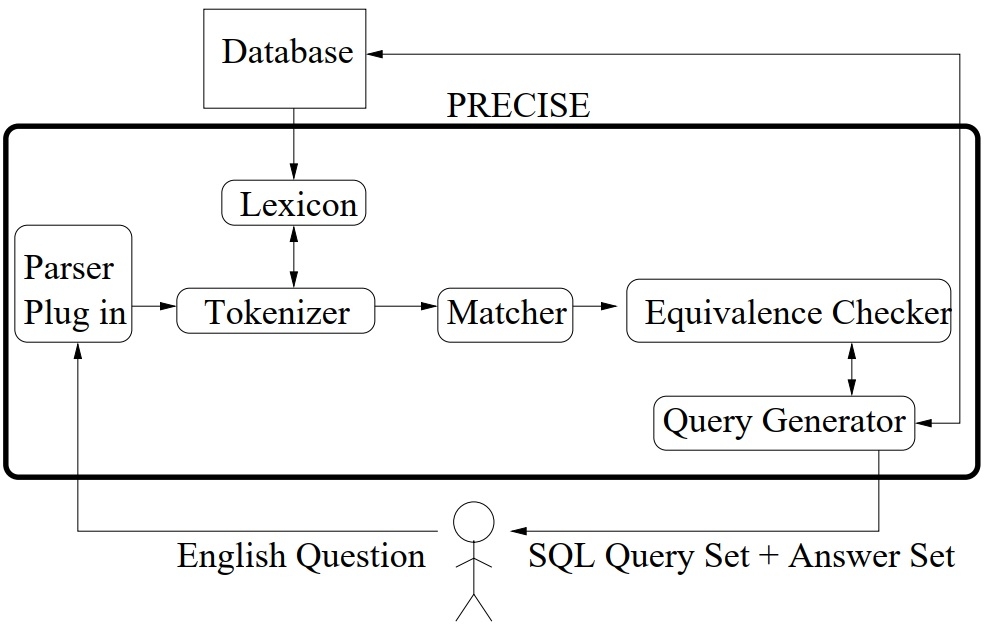
\includegraphics[width=.65\textwidth]{ch03/assets/precise_architecture.jpg}
    \caption{Arquitetura do sistema PRECISE, extraído de~\textcite{towards_theory_nli_databases}}
    \label{fig:precise_architecture}
\end{figure}

Quanto aos restantes componentes: o \textit{Lexicon} extrai os \textit{tokens} de uma dada frase e encontra sinónimos dessas expressões; o \textit{Tokenizer} verifica se, para cada potencial \textit{token}, outras palavras estão também presentes na questão, e associa-lhes um um determinado tipo de elemento de base de dados (\exempligratia{valor, atributo, relação}); o \textit{Matcher} procede à correspondência entre os \textit{tokens} e os respetivos elementos da base de dados; o \textit{Query Generator}, como o próprio nome indica, é responsável por gerar a \textit{query} de \gls{sql}; o \textit{Equivalence Checker} testa se existem soluções distintas e, em caso de as encontrar, o sistema questiona o utilizador acerca da interpretação semântica da questão~\parencite{towards_theory_nli_databases}.

Este sistema foi avaliado em dois domínios: o primeiro, referente a viagens aéreas e o segundo, associado à geografia dos Estados Unidos da América. De acordo com \textcite{nlidb_brief_review}, no primeiro caso, $95.8\%$ das questões são semanticamente tratáveis, pelo que a precisão do sistema atinge os $94\%$ e, no segundo caso, $77.5\%$ das questões são tratáveis em termos de semântica, obtendo $100\%$ de precisão, destacando-se assim o seu desempenho.

\subsection{NALIX}
O NALIX -- \textit{Natural Language Interface for an XML Database} -- é uma \gls{ilnbd} desenvolvida na Universidade de Michigan, com o intuito de obter informação genérica a partir de uma base de dados em \gls{xml}~\parencite{nalix_interactive_nli_querying_xml}. De acordo com~\textcite{nalix_interactive_nli_querying_xml}, o desafio consiste em traduzir uma \textit{query} de linguagem natural para uma \textit{query} corretamente estruturada para uso numa base de dados, permitindo assim ao utilizador usar operações complexas (\exempligratia{agregação, combinação, junção, entre outras}).

Relativamente à arquitetura do NALIX (Figura~\ref{fig:nalix_architecture}), o sistema consiste em duas partes: a primeira é responsável pela tradução da \textit{query} de linguagem natural para XQuery\footnote{Disponível em \url{https://www.w3schools.com/xml/xquery_intro.asp}.}, envolvendo os componentes \textit{Parse Tree Classifier}, \textit{Parse Tree Validator} e \textit{Parse Tree Translator}; a segunda suporta a formulação da \textit{query} de base de dados correspondente, usando os componentes \textit{Query Repository} e \textit{Message Generator}~\parencite{nalix_interactive_nli_querying_xml}.

\begin{figure}[!ht]
    \centering
    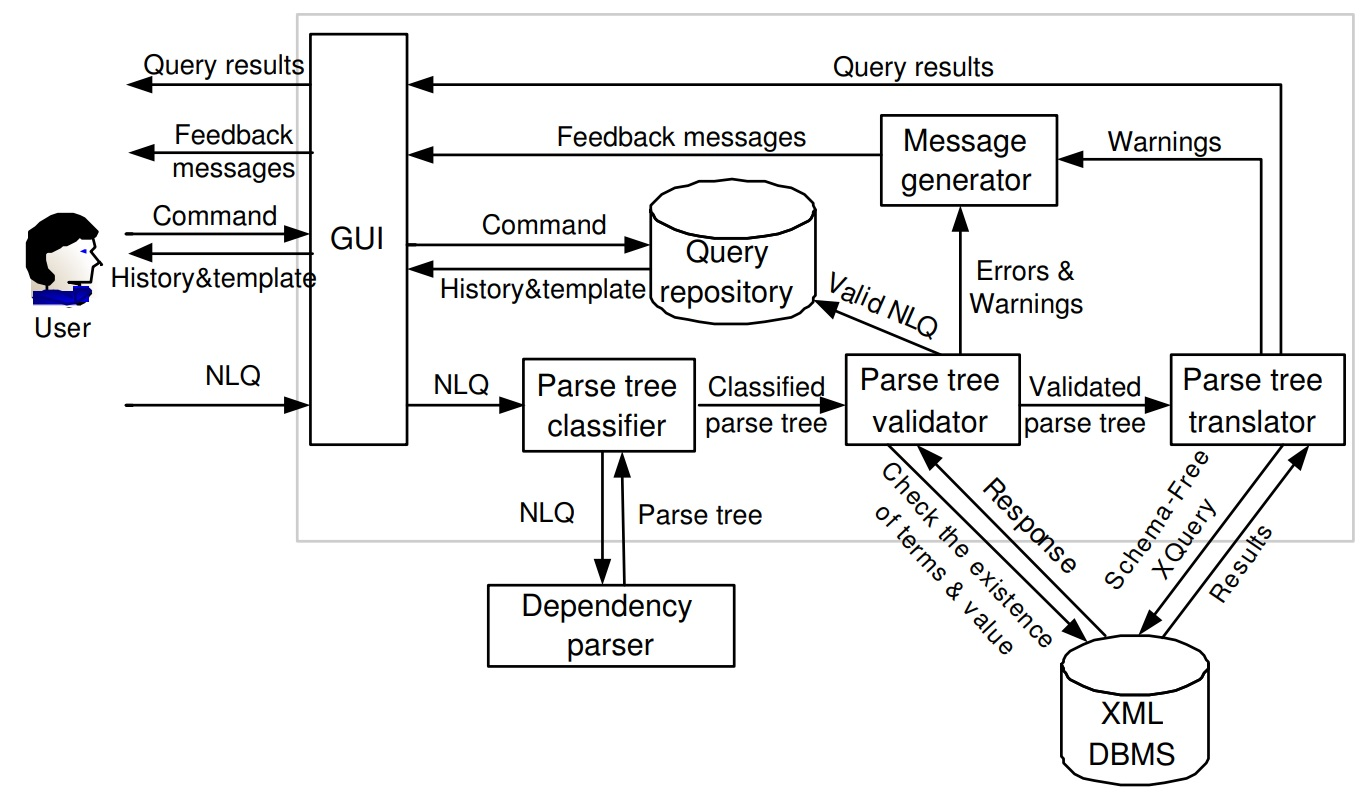
\includegraphics[width=.7\textwidth]{ch03/assets/nalix_architecture.jpg}
    \caption{Arquitetura do sistema NALIX, extraído de~\textcite{nalix_interactive_nli_querying_xml}}
    \label{fig:nalix_architecture}
\end{figure}

De salientar é que a linguagem de \textit{query} usada pelo NALIX (\textit{Schema Free XQuery}) não necessita que seja explicitado qual o \textit{schema} a ser usado, sendo que é capaz de encontrar automaticamente, para uma dada coleção de expressões/palavras-chave, todas as relações existentes entre estes elementos. Assim, é possível abstrair o sistema do domínio existente~\parencite{nalix_interactive_nli_querying_xml, survey_nlidb}.

\subsection{GINLIDB}
Este sistema -- \textit{Generic Interactive Natural Language Interface to Databases} -- foi desenvolvido em 2009 com o propósito de ser genérico o suficiente para se adaptar a bases de dados diferentes, dada a base de conhecimento apropriada~\parencite{ginlidb}. A arquitetura do GINLIDB, apresentada na Figura~\ref{fig:ginlidb_architecture}, consiste em dois principais componentes: \textit{Linguistic Handling Component}, o qual gere a exatidão da \textit{query} de linguagem natural, nomeadamente a estrutura gramatical e possibilidade de ser corretamente convertida para \gls{sql}; \textit{SQL Construting Component}, responsável por construir a \textit{query} de \gls{sql} apropriada e gerir a ligação à base de dados~\parencite{ginlidb}.

\begin{figure}[!ht]
    \centering
    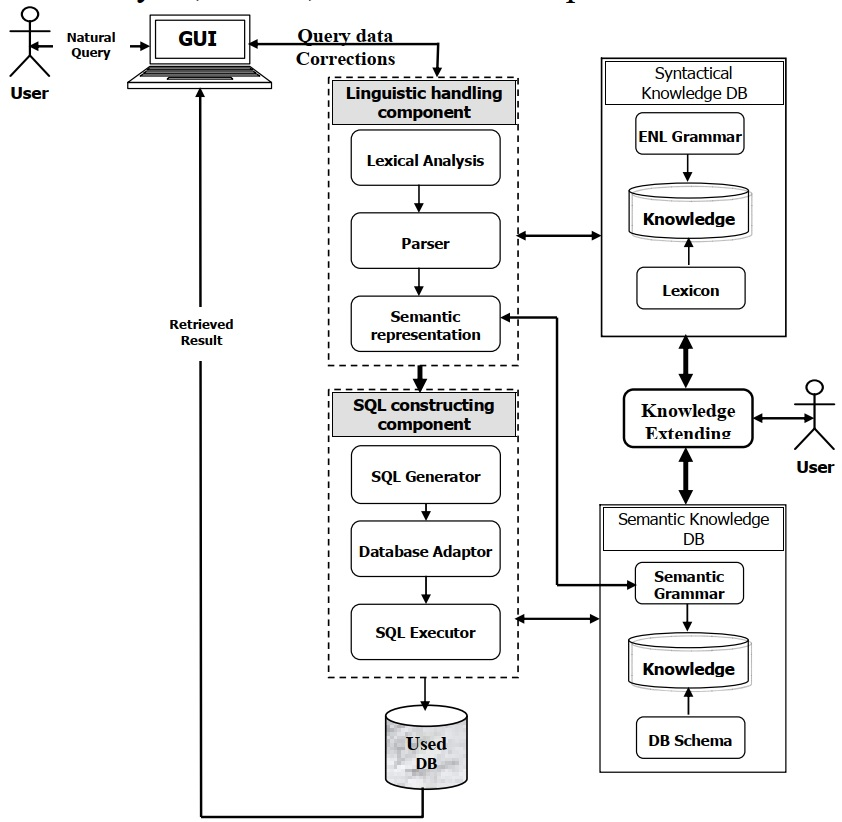
\includegraphics[width=.62\textwidth]{ch03/assets/ginlidb_architecture.jpg}
    \caption{Arquitetura do sistema GINLIDB, extraído de~\textcite{ginlidb}}
    \label{fig:ginlidb_architecture}
\end{figure}

O GINLIDB destaca-se pelo seu processo de análise sintática, no qual usa \gls{atn}, que verifica se a estrutura dos \textit{tokens} é permitida na estrutura gramatical. Este processo é suportado pelo \textit{parser} desenvolvido para o sistema usando uma gramática de contexto livre. Outro destaque deste sistema diz respeito à base de conhecimento usada, que é extensível pelo utilizador, permitindo adicionar novas palavras no dicionário, associar-lhes os respetivos sinónimos e definir o \textit{schema} da base de dados em uso, mapeando assim o domínio. Em termos de resultados, o sistema mostrou-se capaz de responder às questões mais comuns, embora não tenha sido testado em diferentes domínios~\parencite{ginlidb}.

\subsection{Sinopse}
Na tabela apresentada em seguida, descriminam-se os casos de estudo abordados anteriormente, focando especialmente a abordagem utilizada e a respetiva técnica.

\begin{table}[!ht]
\caption{Sumário dos casos de estudo de \glsfirst{ilnbd}, baseado em \textcite{survey_nlidb}}
\label{tab:study_cases}
\centering
\resizebox{\textwidth}{!}{
\renewcommand{\arraystretch}{1.25}
\footnotesize
\begin{tabular}{l|l|l|l|l}
%
\toprule
%
\tabhead{Ano}&\tabhead{Nome}&\tabhead{Domínio}&\tabhead{Abordagem}&\tabhead{Técnica}\\ 
%
\midrule
1973 &   LUNAR &   Amostras de rochas da Lua &   bla &   bla\\
1978 &   LADDER &   Navios da Marinha Americana  &   bla &   bla\\
1980 &   CHAT-80 &   Genérico &   bla &   bla\\
1989 &   JANUS &   Genérico &   bla &   bla\\
2004 &   PRECISE &   Viagens aéreas e geografia &   bla &   bla\\
2006 &   NALIX &   Genérico &   bla &   bla\\
2009 &   GINLIDB &   Genérico &   bla &   bla\\
%
\bottomrule
\end{tabular}
}
\end{table}

Uma análise cuidada sobre os projetos apresentados na Tabela~\ref{tab:study_cases} demonstra que não existe uma abordagem ou técnica recorrente. Para a solução a desenvolver, qualquer das combinações pode ser válida, pelo que a integração com técnicas mais recentes de \gls{ml} ou \gls{dl} podem constituir um novo passo na implementação de \gls{ilnbd}. Nesse sentido, o uso de ferramentas \gls{pln} já existentes ou o desenvolvimento de raiz de uma para esse efeito são alternativas a ser consideradas e cuja conceção da solução irá ter em consideração.

%%%%%%%%%%%%%%%%%%%%%%%%%%%%%%%%%
%           SECTION
%%%%%%%%%%%%%%%%%%%%%%%%%%%%%%%%%
\section{Ferramentas para Processamento de Linguagem Natural}
\label{sec:chap03_existingtools}
Atualmente, são disponibilizadas várias ferramentas para lidar com o \gls{pln}, sendo que se torna necessário destacar as mais relevantes e perceber qual pode ser a mais adequada na resolução do problema , dadas as particularidades de cada uma. Posteriormente, faz-se o comparativo de todas as ferramentas, selecionando aquela que se revela ser a mais apropriada, usando uma matriz de decisão para o efeito.

\subsection{NLTK}
O NLTK, \textit{Natural Language Toolkit}, foi criado em 2001 na Universidade da Pennsylvania e, desde então, tem-se expandido graças à comunidade \textit{open source} que contribui para o projecto~\parencite{applied_natural_language_processing_with_python}. Esta biblioteca, desenvolvida em \textit{Python} para processamento de linguagem natural e análise textual, caracteriza-se pela sua simplicidade, consistência, extensibilidade e modularidade, apresentando um conjunto de funções otimizadas para suportar estas tarefas listadas~\parencite{applied_natural_language_processing_with_python, python_text_processing_nltk_cookbook}. De acordo com~\textcite{nltk_education_scientific_purposes}, a combinação de \textit{Python} e NLTK dá a capacidade a qualquer programador de resolver facilmente tarefas de \gls{pln}, evitando demasiado tempo a  estudar os conceitos inerentes. Neste contexto, a biblioteca está integrada com \textit{WordNet}\footnote{Disponível em \url{https://wordnet.princeton.edu/}}, uma base de dados de relações semânticas entre nomes, verbos, adjetivos e advérbios da Língua Inglesa~\parencite{nltk_education_scientific_purposes}.

O NLTK providencia poderosas ferramentas estatísticas, está preparado para trabalhar com grandes \textit{datasets}, criar modelos linguísticos robustos, possibilitando a sua extensão para componentes que possam ser usados em sistemas produtivos~\parencite{nltk_education_scientific_purposes, applied_natural_language_processing_with_python}.

\subsection{Stanford CoreNLP}
O Stanford CoreNLP é uma \textit{framework} que providencia um conjunto de ferramentas para analisar discurso, reconhecer entidades, normalizar datas, identificar a estrutura frásica e dependência sintática dos termos, entre outras~\parencite{stanford_open_nlp}. Ele possui uma \gls{api} rica, sendo assim acessível em múltiplas linguagens de programação e é a biblioteca mais usada em projetos de pesquisa cuja temática é o \gls{pln}~\parencite{stanford_open_nlp, choosing_nlp_library}.

\subsection{spaCy}
O spaCy é uma biblioteca para métodos avançados de processamento de linguagem natural, desenvolvida com \textit{Python} e \textit{CPython}, e cujo objetivo é suportar a conceção de aplicações de foro comercial~\parencite{choosing_nlp_library}. Esta biblioteca suporta as funcionalidades de \gls{pln} a partir de modelos estatísticos pré-treinados especificamente para o spaCy, tornando-o rápido e preciso~\parencite{spacy_usage}.

\subsection{TensorFlow}
O projeto Google Brain\footnote{Disponível em \url{https://ai.google/research/teams/brain/}} começou, em 2011, com o objetivo de explorar redes neuronais de larga escala, quer para pesquisa, quer para uso nos produtos da Google~\parencite{tensorflow_largescale_machine_learning_distributed_systems}. O TensorFlow é um sistema de segunda geração, sucessor do DistBelief\footnote{Disponível em \url{https://ai.google/research/pubs/pub40565}}, usado para a implementação e implantação de modelos de \gls{ml} de elevada escala~\parencite{tensorflow_largescale_machine_learning_distributed_systems}. Este usa grafos \textit{dataflow}, um modelo de grafo que expressa as possibilidades de execução concorrente de partes de um programa, para representar computacionalmente o estado partilhado e as operações responsáveis pela mutação desse estado, o que inclui operações matemáticas individuais, os respetivos parâmetros, as suas regras de atualização e o pré-processamento dos dados de entrada~\parencite{data_flow_graphs_encyclopedia_parellel_computing, tensorflow_system_largescale_machine_learning}.

Num contexto de \gls{pln}, usando TensorFlow, pode aplicar-se redes neuronais convolucionais para tarefas de classificação, como análise de sentimento, deteção de \textit{spam} ou categorização de tópicos~\parencite{understanding_convolution_neural_networks_nlp}. Embora as redes neuronais convolucionais sejam tipicamente usadas na identificação de imagens, podem também ser usadas em tarefas \gls{pln}, usando as palavras como entrada, ao invés dos pixeis, sendo a sua computação rápida e eficiente~\parencite{understanding_convolution_neural_networks_nlp}.

\subsection{Rasa}
O Rasa é uma \textit{framework} \textit{open source} que permite o desenvolvimento de \textit{chatbots}, possibilitando, entre muitas outras capacidades, a compreensão de intenções e entidades envolvidas na conversação~\parencite{rasa_official}. Esta \textit{framework} baseia algumas das suas funcionalidades em ferramentas \gls{pln} já existentes, dando-lhe flexibilidade nas tarefas inerentes à compreensão da linguagem natural~\parencite{rasa_open_source_language_understanding}. Também importante referir que o Rasa é modular, ou seja, é constituído por dois componentes: o Rasa NLU, responsável pela compreensão da linguagem, classificando intenções e extraindo entidades; o Rasa Core, o motor de construção de diálogos; sendo possível usar cada um deles em conjunto ou isoladamente, facilitando também a integração com outros sistemas~\parencite{rasa_open_source_language_understanding, rasa_official}. O domínio consumido pelo Rasa é configurável, através de ficheiros \gls{json} ou \textit{Markdown}, e os seus componentes disponibilizam uma \gls{api} apoiada em \gls{http}, o que contribui para a escalabilidade e facilidade de integração do sistema, respetivamente~\parencite{rasa_open_source_language_understanding}.

\subsection{Amazon Lex}
O Lex é um produto do \textit{Amazon Web Services} (mais conhecida como AWS), uma plataforma de serviços da Amazon na \textit{cloud}, para construir interfaces de conversação integradas com qualquer aplicação, usando voz ou texto, fornecendo funcionalidades de reconhecimento automático de discurso, respetiva conversão para texto e compreensão de linguagem natural, o que possibilita a identificação das intenções manifestadas pelo utilizador, duma forma simples de usar, implantar e escalar~\parencite{amazon_lex_official}. Como demonstrado em~\textcite{aws_ml_blog_conversational_business}, o Amazon Lex garante a sua customização por forma a desenvolver um \textit{chatbot} capaz de interagir com o utilizador, convertendo os seus pedidos de linguagem natural para \gls{sql}, obtendo os dados de uma base de dados relacional, e por fim, apresentá-los.

\subsection{IBM Watson Assistant}
O Watson Assistant é um produto do IBM Watson, um plataforma de serviços na \textit{cloud}, orientados à inteligência artificial e disponibilizado pela IBM~\parencite{ibm_watson_official}. Este produto oferece uma interface de conversação que pode ser integrada em qualquer aplicação ou dispositivo, e tal como os seus concorrentes, destaca-se por usar técnicas avançadas de compreensão de linguagem natural (suportando intenções e entidades), por ser simples de implantar e fácil de usar~\parencite{ibm_watson_assistant_official}. O IBM Watson Assistant também permite a conceção de \textit{chatbots} capazes de interpretar o pedido do utilizador e extrair o conteúdo desejado de uma base de dados~\parencite{ibm_watson_assistant_database_driven_chatbot}.

\subsection{Microsoft LUIS}
O LUIS, acrónimo para \textit{Language Understanding Intelligent Service}, é um serviço da Microsoft, baseado na \textit{cloud} e parte do produto \textit{Cognitive Services}, e que por sua vez integra na plataforma Azure, que aplica métodos de \gls{ml} à linguagem natural, permitindo obter informação relevante acerca da mesma~\parencite{microsoft_luis_official}. O intuito do LUIS é tornar possível a criação de soluções que apliquem modelos específicos de \gls{ml} para a compreensão de linguagem específica de um determinado domínio, sem qualquer tipo de perícia nesta área~\parencite{luis_fast_easy_language_understanding}. Assim, o LUIS permite a construção do próprio modelo, através da identificação de entidades, de intenções e das frases que lhes são associadas, oferecendo diversas ferramentas ao desenvolvedor para que este processo seja mais simples~\parencite{microsoft_luis_official}. Relativamente à sua aplicabilidade ao problema, a combinação do LUIS com o QnA Maker (outro serviço integrante do \textit{Cognitive Services}) resulta numa solução capaz de identificar as intenções e entidades, entregando respostas pré-fabricadas ou informação de uma determinada fonte~\parencite{microsoft_luis_use_nl_processing_service}.

\subsection{Sinopse}
As ferramentas apresentadas previamente podem ser divididas por tipo; as cinco primeiras referem-se a bibliotecas ou \textit{frameworks} -- NLTK, Stanford CoreNLP, spaCy, TensorFlow e Rasa --, as últimas três dizem respeito a serviços disponibilizados na \textit{cloud} - Amazon Lex, IBM Watson Assistant e Microsoft LUIS. Por essa razão, sendo que o objetivo é perceber qual a ferramenta mais adequada, é importante notar que a natureza de cada uma é diferente, o que influencia o comparativo entre elas. Portanto, essa comparação não deve ser feita pelas funcionalidades que cada uma oferece, mas sim pelo o valor que poderá trazer à solução, ou seja, pelos critérios e/ou restrições que cumprem.

Para auxiliar no processo de decisão, opta-se pelo uso de uma matriz de decisão, uma ferramenta que permite identificar rapidamente a melhor alternativa, a partir de um conjunto pré-definido de critérios e da escala de avaliação~\parencite{decisions_engineering_design}.
Para os critérios de avaliação consideram-se que têm todos o mesmo grau de importância, pelo que são descritos a seguir.

\begin{itemize}
    \item
    {
        \textit{Dependência} -- a nível de plataforma, linguagem de programação, ambiente de desenvolvimento, acesso à Internet ou outras;
    }
    \item
    {
        \textit{Custo} -- possível preço da solução e/ou gastos com recursos;  
    }
    \item
    {
        \textit{Facilidade} -- utilização na perspetiva do programador, ou seja, se apresenta boa documentação, fácil e rápido de aprender e desenvolver;
    }
    \item
    {
        \textit{Esforço} -- dispêndio no desenvolvimento da solução. Ferramentas com modelos pré-treinados necessitarão de menos esforço do que ferramentas que não os forneçam;
    }
    \item
    {
        \textit{Escalabilidade} -- como é que a ferramenta se comporta quando a aplicação tem a necessidade de escalar, ou seja, se o nível de eficiência ou a facilidade de desenvolvimento se mantém constante.
    }
\end{itemize}

Quanto à escala de avaliação, opta-se por três níveis: um ($1$) até três ($3$), para indicar a baixa e elevada adequabilidade, respetivamente. Por exemplo, se para o critério \textit{Custo} a pontuação dada é um ($1$), significa que o item/ferramenta, nesse critério, é pouco adequado para a solução. A soma de todas as pontuações define a adequabilidade da ferramenta. Quanto mais alta for, mais adequada é. De salientar que a avaliação é feita com base na bibliografia recolhida para as ferramentas estudadas. Na Tabela~\ref{tab:tools_comparison} apresenta-se a matriz de decisão para as ferramentas estudadas anteriormente.

\begin{table}[!ht]
\caption{Comparativo das ferramentas de processamento de linguagem natural}
\label{tab:tools_comparison}
\centering
\resizebox{\textwidth}{!}{
\renewcommand{\arraystretch}{1.3}
\footnotesize
\begin{tabular}{l*6{|c}}
%
\toprule
%
\tabhead{Ferramenta}&\tabhead{Dependência}&\tabhead{Custo}&\tabhead{Facilidade}&\tabhead{Esforço}&\tabhead{Escalabilidade}&\tabhead{Pontuação}\\
%
\midrule
NLTK&$1$&$3$&$1$&$1$&$2$&$8$\\
%
Stanford CoreNLP&$1$&$3$&$1$&$1$&$1$&$7$\\
%
spaCy&$2$&$3$&$2$&$2$&$3$&$12$\\
%
TensorFlow&$2$&$3$&$1$&$1$&$3$&$10$\\
%
Rasa&$2$&$3$&$2$&$2$&$3$&$12$\\
%
Amazon Lex&$1$&$1$&$3$&$3$&$3$&$11$\\
%
IBM Watson Assistant&$1$&$1$&$3$&$3$&$3$&$11$\\
%
Microsoft LUIS&$1$&$1$&$3$&$3$&$3$&$11$\\
\bottomrule
\end{tabular}

}
\end{table}

A matriz de decisão apresentada na Tabela~\ref{tab:tools_comparison} aponta o spaCy e o Rasa como as ferramentas mais adequadas para o módulo de linguagem natural, pois cumprem a maioria dos critérios e não se tratam de ferramentas na \textit{cloud}, visto que esta última é uma restrição da empresa. Em suma, tanto o spaCy como o Rasa são bons candidatos para o desenvolvimento da solução final, embora possam existir ferramentas mais adequadas no mercado, que são desconhecidas, e por isso, não contempladas no estudo. É importante salientar que o uso isolado do spaCy pode não ser suficiente para responder a todas as necessidades ou casos de uso do sistema, pelo que a integração com outras ferramentas pode ser preferida, sendo assim necessário um estudo mais aprofundado sobre os conceitos teóricos abrangidos nesta ferramenta. Já no caso do Rasa, os módulos disponibilizados parecem ser suficientes para a resolução do problema, sendo importante estudar com mais detalhe esta \textit{framework}.

No contexto desta tese, como prova de conceito, o uso de uma ferramenta na \textit{cloud} é aceitável -- o Microsoft LUIS, por exemplo --, visto que se pretende validar uma abordagem. Teoricamente, o reconhecimento de intenções e entidades, uma abordagem seguida pelas ferramentas da \textit{cloud} e que estão indicadas na bibliografia, parece constituir uma forma robusta de responder ao problema, pelo que poderão ser exploradas na prática.

%%%%%%%%%%%%%%%%%%%%%%%%%%%%%%%%%
%           SECTION
%%%%%%%%%%%%%%%%%%%%%%%%%%%%%%%%%
\section{Síntese do Capítulo}
\label{sec:chap03_chaptersummary}

\chapter{Conceção}
\label{chap:Chapter4}
Neste capítulo apresenta-se o processo de idealização do modelo de \glsfirst{iln}. Inicialmente, mostra-se o processo de experimentação de algumas ferramentas ou abordagens analisadas no capítulo anterior, procurando perceber se a sua aplicação prática é plausível. Depois, apresenta-se o modelo concetualizado, concretamente a visão geral, em que se faz uma descrição do modelo na sua globalidade, os casos de uso identificados e por fim, a arquitetura definida.

%%%%%%%%%%%%%%%%%%%%%%%%%%%%%%%%%
%           SECTION
%%%%%%%%%%%%%%%%%%%%%%%%%%%%%%%%%
\section{Apreciação Prática}
\label{sec:chap04_approaches}
Com o propósito de colocar em prática o estudo das \glspl{iln}, decidiu-se realizar experiências envolvendo algumas abordagens e ferramentas previamente estudadas (ver Capítulo~\ref{chap:Chapter3}). Posto isto, optou-se por desenvolver pequenas provas de conceito, num período bem definido, de forma a fazer uma rápida avaliação das abordagens, técnicas e ferramentas usadas. Para cada uma, é abordado em que consiste, algumas observações pertinentes e referência dos pontos favoráveis e desfavoráveis.

\subsection{Gramática Baseada em Semântica}
Como proposto em~\textcite[p.~361-403]{natural_language_processing_with_python}, o uso do NLTK permite o desenvolvimento de gramáticas que possibilitam a análise de uma frase pela sua semântica, tal como o exemplo demonstrado a seguir.

\begin{lstlisting}[language=Python,caption={Excerto de uma gramática extraída de~\textcite{natural_language_processing_with_python}},numbers=none,label=lst:grammarexample,basicstyle=\scriptsize]
S[SEM=(?np + WHERE + ?vp)] -> NP[SEM=?np] VP[SEM=?vp]
VP[SEM=(?v + ?pp)] -> IV[SEM=?v] PP[SEM=?pp]
VP[SEM=(?v + ?ap)] -> IV[SEM=?v] AP[SEM=?ap]
NP[SEM=(?det + ?n)] -> Det[SEM=?det] N[SEM=?n]
PP[SEM=(?p + ?np)] -> P[SEM=?p] NP[SEM=?np]
AP[SEM=?pp] -> A[SEM=?a] PP[SEM=?pp]
NP[SEM='Country="greece"'] -> 'Greece'
NP[SEM='Country="china"'] -> 'China'
Det[SEM='SELECT'] -> 'Which' | 'What'
N[SEM='City FROM city_table'] -> 'cities'
IV[SEM=''] -> 'are'
A[SEM=''] -> 'located'
P[SEM=''] -> 'in'
\end{lstlisting}

O código apresentado em~\ref{lst:grammarexample}, usando o NLTK, para a pergunta \inquotes{What cities are located in China?} permite gerar a seguinte \textit{query} de \gls{sql}: SELECT City FROM city\_table WHERE Country=\inquotes{china}. Com esta metodologia é possível mapear diretamente linguagem natural em \gls{sql}, sendo que a gramática funciona como a base de conhecimento. Por conseguinte, torna-se viável a codificação de um \textit{parser} que usa as gramáticas definidas, verificando
alguma é capaz de dar resposta à \textit{query} de linguagem natural.

\subsubsection*{Pontos Favoráveis}
\begin{itemize}
    \item 
    {
        Viabilidade de desenvolvimento de uma solução customizada;
    }
    \item
    {
        Utilização de ferramenta \textit{open source};
    }
    \item 
    {
        Tradução imediata de linguagem natural para \gls{sql}. 
    }
\end{itemize}

\subsubsection*{Pontos Desfavoráveis}
\begin{itemize}
    \item 
    {
        Dificuldade em criar ou estender gramáticas;
    }
    \item
    {
        Complexidade em adaptar para múltiplas línguas ou domínios;
    }
    \item
    {
        Necessidade de conhecimento linguístico, por forma a adaptar a gramática às regras de uma determinada língua;
    }
    \item
    {
        Ambiguidade da semântica. Diferentes expressões podem ou devem gerar o mesmo \gls{sql};
    }
    \item
    {
        Manutenção difícil.
    }
\end{itemize}

\subsection{Pesquisa Semântica}
Nesta abordagem foi usada uma \textit{framework} que não consta nas ferramentas estudadas (ver Secção~\ref{sec:chap03_existingtools}), principalmente porque o seu desenvolvimento encontra-se estagnado desde 2013. Ainda assim, é aceitável o seu uso para testar esta mesma abordagem, no ponto de vista prático. O Quepy é desenvolvido em \textit{Python} e tem como objetivo a transformação de linguagem natural em \textit{SPARQL Protocol and RDF Query Language} (SPARQL)\footnote{Disponível em \url{https://www.w3.org/TR/rdf-sparql-query/}.} e \textit{Metaweb Query Language} (MQL)\footnote{Disponível em \url{https://github.com/nchah/freebase-mql}.}, linguagens de \textit{query} usadas com tecnologia \gls{rdf}\footnote{Disponível em \url{https://www.w3.org/RDF/}.}, \inquotes{um modelo padrão para permuta de dados na Web}\footnote{Tradução livre do autor. No original \inquotes{is a standard model for data interchange on the Web.}.}, intrinsecamente ligado ao campo da Web Semântica~\parencite{resource_description_framework}.

Neste caso, o uso do Quepy implica a definição da linguagem específica de domínio através de código \textit{Python}, respeitando as restrições colocadas na documentação da \textit{framework}, de maneira a que esta seja capaz de reconhecer o padrão introduzido.

\begin{lstlisting}[language=python, caption={Excerto da definição semântica da frase que lida com listagem de produtos},numbers=none,label=lst:quepyexample,basicstyle=\scriptsize]
from quepy.dsl import FixedType, FixedRelation
from quepy.parsing import Lemma, QuestionTemplate

class NameOf(FixedRelation):
    "Name of the entity's property"
    relation = "product_name"
    reverse = True

class IsProduct(FixedType):
    "Defines the entity's type"
    fixedtype = "product"

class ListProducts(QuestionTemplate):
    "Questions such as 'List products' or 'Listing products'"
    regex = Lemma("list") + Lemma("product")

    def interpret(self, match):
        product = IsProduct()
        name = NameOf(product)
        return name, "enum"

\end{lstlisting}

No excerto demonstrado em~\ref{lst:quepyexample}, define-se a expressão regular que caracteriza a questão esperada, para além de detalhes relacionados com a linguagem específica de domínio. A \textit{query} obtida pode ser posteriormente usada numa base de dados \gls{rdf}, como o objetivo de recolher os dados. De notar que, neste caso, sendo o propósito a consulta de uma base de dados relacional, seria necessária uma forma de a transpor ou replicar numa camada compatível com tecnologia \gls{rdf}. Para isso, existem ferramentas capazes de executar esse mapeamento, como por exemplo o D2RQ\footnote{Disponível em \url{http://d2rq.org/}.}.

\subsubsection*{Pontos Favoráveis}
\begin{itemize}
    \item
    {
        Viabilidade de desenvolvimento de uma solução customizada;
    }
    \item
    {
        Tecnologia \textit{open source};
    }
    \item 
    {
        Linguagem específica de domínio permite abstração aos detalhes de implementação associados ao reconhecimento de linguagem natural;
    }
    \item
    {
        Reconhecimento da linguagem natural é feita através da análise de expressões regulares, o que torna fácil compreender a estrutura frásica;
    }
    \item
    {
        Transformação da linguagem natural numa representação que obedece à especificação da tecnologia \gls{rdf}, definida pela W3C.
    }
\end{itemize}

\subsubsection*{Pontos Desfavoráveis}
\begin{itemize}
    \item
    {
        As regras de domínio e o modelo de dados devem ser definidos diretamente no código, não possibilitando a extensibilidade por configuração;
    }
    \item
    {
        Rigidez da linguagem usada, já que o uso de expressões regulares implica uma estrutura minimamente estática para que o reconhecimento seja bem sucedido;
    }
    \item
    {
        O uso de tecnologias \gls{rdf} levam a uma nova camada aplicacional, que envolve o uso de ferramentas não relacionadas com o \gls{pln} e que leva a mais esforço na manutenção do sistema;
    }
    \item
    {
        Necessidade de estudo aprofundado ou conhecimento pericial na área de Web Semântica.
    }
\end{itemize}

\subsection{Reconhecimento de Intenções e Entidades}
Neste contexto, foi utilizado o Microsoft LUIS. A razão para esta escolha deve-se principalmente a dois fatores: o facto de ser uma das plataformas mais usadas e documentadas e pela Microsoft disponibilizar este tipo de ferramentas a quem possua subscrição de estudante. Para esta prova de conceito criou-se um \textit{chatbot} capaz de responder a algumas perguntas colocadas pelo utilizador (\textit{utterance}), identificando qual a sua intenção (\textit{intent}) e quais as entidades envolvidas (\textit{entity}), descritas na Tabela~\ref{tab:luis_intents}.
%
\begin{table}
\caption{Descrição de algumas das intenções e entidades dada a expressão de exemplo, baseado em~\textcite[Concepts]{microsoft_luis_official}}
\label{tab:luis_intents}
\centering
\resizebox{\textwidth}{!}{
\renewcommand{\arraystretch}{1.3}
\footnotesize
\begin{tabular}{l*{2}{|l}}
%
\toprule
%
\tabhead{Expressão de Exemplo}&\tabhead{Intenção}&\tabhead{Entidades}\\
%
\midrule
%
{Good Morning}&{Greeting}&{--}\\
%
{What's the weather like in \underline{Porto}?}&{CheckWeather}&{Place}\\
%
{Turn on the Internet in my \underline{bedroom}, please}&{HomeAutomation}&{Room}\\
%
{Book me a flight to \underline{Lisbon} \underline{next week}}&{BookFlight}&{Place, Datetime}\\
%
\bottomrule
%
\end{tabular}
}
\end{table}

O \textit{chatbot} recorre ao Microsoft LUIS para identificar a intenção do utilizador, e com base nisso e nas entidades recolhidas, pode carregar os dados necessários e apresentá-los da forma que for mais adequada. Neste caso, o \textit{chatbot} retorna apenas a intenção que foi capaz de identificar (ver Figura~\ref{fig:chatbotexample}).
%
\begin{figure}
\centering
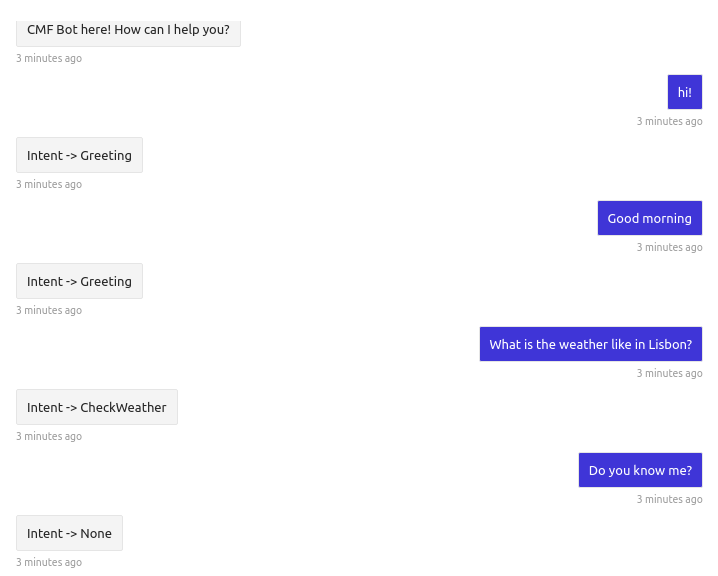
\includegraphics[width=.8\textwidth]{ch03/assets/chatbot.png}
\caption{Resultado do teste com \textit{chatbot} desenvolvido usando Microsoft LUIS}
\label{fig:chatbotexample}
\end{figure}
%
É possível dotar o \textit{chatbot} de comportamento para manipular os metadados obtidos, e assim, obter dados de uma base de dados relacional ou obter dados estáticos dum serviço de respostas pré-fabricadas, tal como o QnA Maker\footnote{Disponível em \url{https://www.qnamaker.ai/}}. É importante frisar que, embora esta abordagem tenha sido aplicada recorrendo a um \textit{chatbot}, por imposição da própria plataforma, tal não é obrigatório na utilização da mesma numa solução customizada. 

\subsubsection*{Pontos Favoráveis}
\begin{itemize}
    \item
    {
        As plataformas disponíveis na \textit{cloud} constituem um ponto de partida para uma solução personalizada;
    }
    \item
    {
        A solução é fácil de desenvolver, estender e integrar;
    }
    \item
    {
        A base de conhecimento pode ser totalmente configurável;
    }
    \item
    {
        Robustez na identificação de intenções e entidades, através do uso de modelos de \gls{ml};
    }
\end{itemize}

\subsubsection*{Pontos Desfavoráveis}
\begin{itemize}
    \item
    {
        A aplicação desta abordagem numa biblioteca customizada implica o estudo teórico de \gls{ml} aplicado ao \gls{pln} e consequentemente, maior esforço de desenvolvimento;
    }
    \item
    {
        A adição de novas intenções à base de conhecimento leva também à adição de comportamento para lidar com os mesmas.
    }
\end{itemize}

\subsection{Sinopse}
As abordagens descritas anteriormente baseiam-se nas observações e experiências realizadas, no ponto de vista prático. Portanto, a conclusão aqui exposta leva em consideração os pontos favoráveis e desfavoráveis de cada uma.

A abordagem que parece a mais adequada é a que diz respeito ao reconhecimento de intenções e entidades, principalmente pela facilidade de compreensão e aplicação do conceito. Além do mais, os pontos desfavoráveis mencionados são de índole operacional, pelo que podem ser superados ou até descartados aquando a conceção e/ou desenvolvimento da solução final. Relativamente às abordagens descartadas, aponta-se que a primeira -- gramática baseada em semântica -- se usada no contexto de uma solução final, será difícil manter o seu desenvolvimento e capacidade de cobrir uma gama aceitável de questões válidas. Já a segunda -- pesquisa semântica --, ainda que assente sobre uma tecnologia especificada e aprovada pelo W3C, necessita de uma camada adicional (\gls{rdf}), contribuindo assim para o aumento do esforço em configuração e manutenção do sistema. Por isso, a terceira abordagem revela-se a mais adequada e será contemplada no protótipo a desenvolver.

%%%%%%%%%%%%%%%%%%%%%%%%%%%%%%%%%
%           SECTION
%%%%%%%%%%%%%%%%%%%%%%%%%%%%%%%%%
\section{Modelo Proposto}
\label{sec:chap04_proposal}
O estudo das \glspl{iln}, associado à aplicação prática de algumas ferramentas e abordagens estudadas, permitiram retirar conclusões relevantes de considerar na conceção do modelo. Nesta secção apresenta-se o modelo idealizado para uma \gls{iln} que permita consulta e pesquisa e estados do processo de fabrico, usando uma abordagem de reconhecimento de intenções e entidades.

\subsection{Visão Geral}
O intuito é especificar um modelo que seja possa ser seguido na futura implementação de uma \gls{iln} integrada no {\productname}, que por sua vez irá permitir a consulta e pesquisa de informação acerca do processo fabril, por parte de operadores de linha, engenheiros de produção e gestores. Como se apresenta na Figura~\ref{fig:generic-vision}, o sistema \gls{mes} disponibiliza uma interface para que o utilizador interaja com ele, através de texto e posteriormente voz, esperando obter informação relevante do processo, no formato que melhor se enquadrar.
%
\begin{figure}[!h]
    \centering
    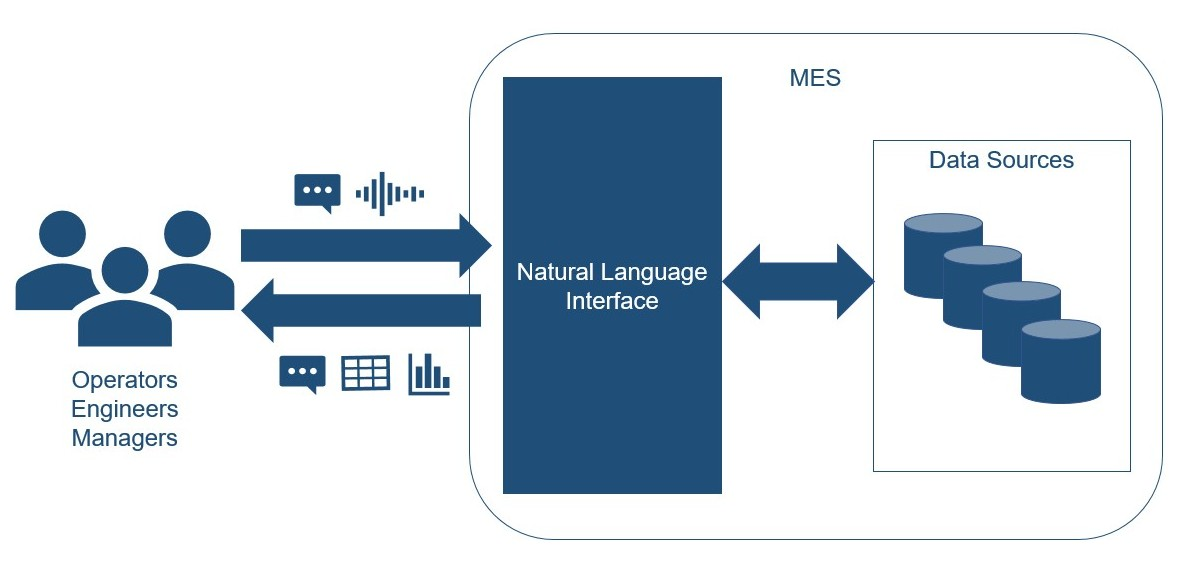
\includegraphics[width=.9\textwidth]{ch04/assets/generic-vision.jpg}
    \caption{Visão da solução desejada para o produto}
    \label{fig:generic-vision}
\end{figure}

O modelo deve ter em conta quatro fatores considerados importantes na possível implementação final: a experiência de utilizador, a extensão da base de conhecimento com o propósito de suportar diferentes domínios, a utilização de \textit{feedback} de utilizador para a aprimoramento da qualidade das respostas geradas e a fácil integração com o {\productname}.

Relativamente à estratégia de reconhecimento de intenções e entidades a ser aplicada no modelo, definem-se os conceitos que lhe estão inerentes, apresentados na Figura~\ref{fig:domain_model}:

\begin{itemize}
    \item 
    {
        \textit{Dynamic Knowledge Base} -- Base de conhecimento dinâmica. Fonte de dados que liga as expressões às intenções e entidades correspondentes e é usado no treino dos modelos \gls{ml} para previsão;
    }
    \item 
    {
        \textit{Static Knowledge Base} -- Base de conhecimento estática. Dicionário onde consta um determinada expressão e respetiva resposta. Pode ser usada para implementar conversação casual ou lidar com expressões que não constam na base de dados dinâmica;
    }
    \item 
    {
        \textit{Intention} -- Intenção. Mapeia ação que o utilizador deseja executar. Normalmente estão-lhe associadas diversas expressões;
    }
    \item 
    {
        \textit{Expression} -- Expressão. Corresponde ao exemplo de estrutura de uma pergunta que o utilizador pode fazer;
    }
    \item 
    {
        \textit{Entity} -- Entidade. Tipicamente refere-se a um conceito de domínio ou do mundo real;
    }
    \item 
    {
        \textit{Static Answer} -- Resposta Estática. Definida na base de conhecimento estática, associada a diferentes expressões. Por exemplo, expressões como \inquotes{Olá} ou \inquotes{Viva} podem ter associadas a respostas como \inquotes{Oi} e \inquotes{Olá}.
    }
\end{itemize}
%
\begin{figure}
    \centering
    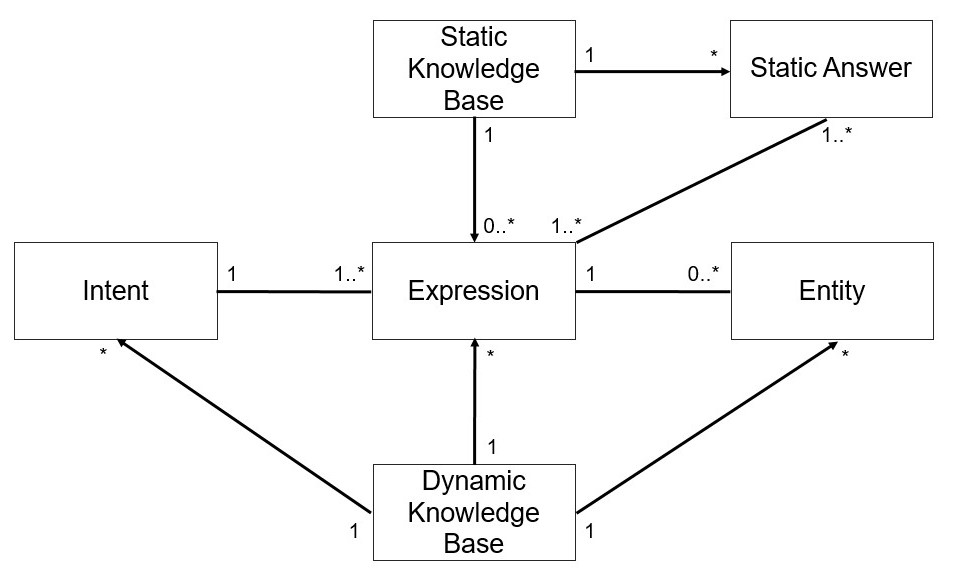
\includegraphics[width=.9\textwidth]{ch04/assets/domain-model.jpg}
    \caption{Conceitos associados ao reconhecimento de intenções e entidades e os respetivos relacionamentos}
    \label{fig:domain_model}
\end{figure}
%
Portanto, uma intenção é um conceito composto, base do modelo, que se apresenta como uma indireção face à questão colocada pelo utilizador, ou seja, a questão é analisada pela ação que lhe está associada e não propriamente pelo seu significado. Desta forma, possibilita-se a escalabilidade e a generalização de domínio, \idest{um pedido para obter os materiais mais fabricados num determinado setor constitui uma intenção única, apesar de apresentar entidades diferentes, consoante o domínio}.

\subsection{Casos de Uso}
De um ponto de vista de utilização, o modelo aqui proposto deve saber lidar com \textit{Perguntas}, \textit{Respostas} e \textit{Feedback}, que se podem considerar as principais áreas funcionais de sistema. Todas têm implicações no bom funcionamento do modelo, sendo que a última, ainda que não seja essencial, é importante na medida em que contribui para melhoria contínua do sistema. Em relação às \textit{Perguntas} e \textit{Respostas}, uma vez que estão profundamente ligadas, apresentando funcionalidades comuns, são então enquadradas numa área funcional única, denominada \textit{Q\&A}. A Figura~\ref{fig:use_cases} dá uma visão geral das áreas funcionais do sistema.
%
\begin{figure}
    \centering
    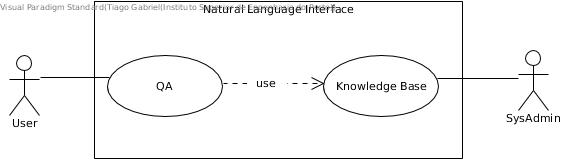
\includegraphics[width=.9\textwidth]{ch04/assets/use-cases.jpg}
    \caption{Áreas funcionais de sistema}
    \label{fig:use_cases}
\end{figure}

As áreas funcionais são descritas em seguida:

\begin{itemize}
    \item 
    {
        \textit{Q\&A} -- corresponde ao conjunto de funcionalidades relacionadas com as perguntas colocadas pelos utilizadores e respetiva procura de respostas;
    }
    \item 
    {
        \textit{Feedback} -- conjunto de funções de sistema que lida com a recolha de \textit{feedback} do utilizador, para contribuir para a melhoria contínua da qualidade das respostas;
    }
    \item 
    {
        \textit{Knowledge Base} -- área funcional \textit{Base de Conhecimento}. Apresenta funcionalidades para a gestão de intenções, expressões, entidades, ou seja, tudo o que as restantes áreas funcionais necessitam para o seu funcionamento.
    }
\end{itemize}

A área funcional \textit{Q\&A} é essencial no contexto deste trabalho, já que se trata da base de interação com o utilizador. Por isso, a Figura~\ref{fig:detailed_use_cases}, apresentada em seguida, detalha algo mais essa área funcional.
%
\begin{figure}[!h]
    \centering
    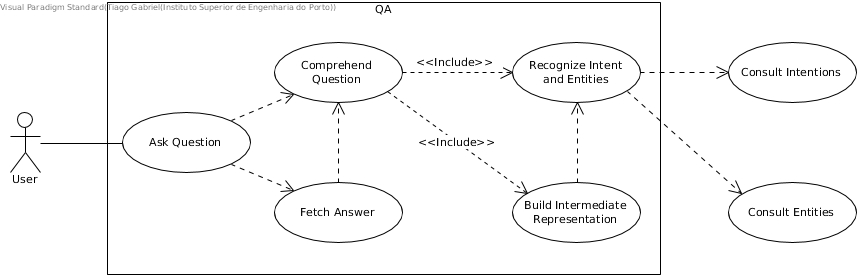
\includegraphics[width=\textwidth]{ch04/assets/questions-use-cases.jpg}
    \caption{Casos de uso identificados para a área funcional \textit{Q\&A}}
    \label{fig:detailed_use_cases}
\end{figure}

Os casos de uso apresentados no diagrama são descritos a seguir:

\begin{itemize}
    \item 
    {
        \textit{Ask Question} -- Fazer Pergunta. É a funcionalidade principal. O utilizador faz a pergunta com o objetivo de obter a resposta que procura. Depende da compreensão da pergunta e da obtenção de resposta;
    }
    \item 
    {
        \textit{Comprehend Question} -- Compreender a Pergunta. O sistema procura compreender a pergunta feita e traduz para uma representação passível de ser usada na fase de procura da resposta nas fontes de dados disponíveis;
    }
    \item 
    {
        \textit{Recognize Intent and Entities} -- Reconhecer a Intenção e as Entidades. O sistema faz o reconhecimento da intenção e das entidades da pergunta feita com base nos modelo de \gls{ml} treinado com os dados que constam na base de conhecimento;
    }
    \item 
    {
        \textit{Build Intermediate Representation} -- Construir Representação Intermédia. O sistema constrói uma representação intermediária que contém os metadados da pergunta colocada -- intenção, entidades e outros dados relevantes;
    }
    \item 
    {
        \textit{Consult Intentions} -- Consultar as Intenções. Permite a consulta de intenções mantidas na base de conhecimento;
    }
    \item 
    {
        \textit{Consult Entities} -- Consultar as Entidades. Permite a consulta as entidades mantidas na base de conhecimento;
    }
    \item 
    {
        \textit{Fetch Answer} -- Obter a Resposta. O sistema usa o resultado (representação intermediária) da fase de compreensão da pergunta para converter essa representação numa compatível com a fonte de dados a interagir, obtendo assim a resposta.
    }
\end{itemize}

Os casos de uso apresentados são a base das funcionalidades do modelo, e por isso, serão explorados em contexto prático no capítulo seguinte.

\subsection{Arquitetura}
Dada a visão geral do modelo e dos seus casos de uso, pretende-se expor a estrutura da solução numa perspetiva lógica, partindo do pressuposto que será o modelo usado na solução final a desenvolver para o {\productname}. Assim, a Figura~\ref{fig:prototype_architecture} demonstra a arquitetura do modelo, primeiro num vista a alto nível e depois mais focado no elemento principal, explicando a responsabilidade inerente a cada componente.
%
\begin{figure}
\centering
    \begin{subfigure}{\textwidth}
         \centering
         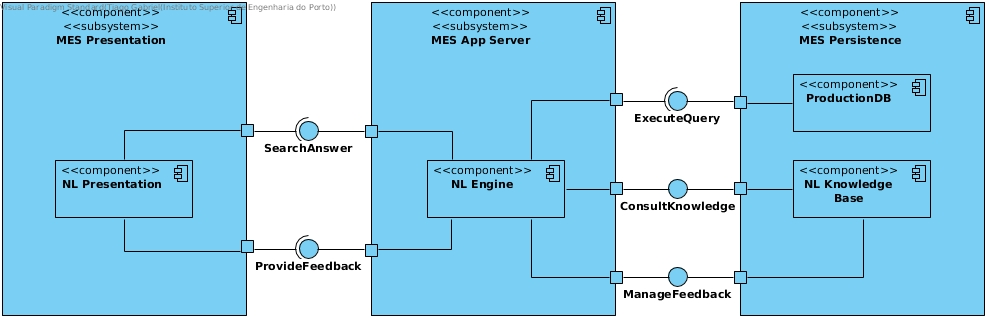
\includegraphics[width=\textwidth]{ch04/assets/generic-architecture.jpg}
         \caption{Arquitetura genérica do protótipo}
         \label{fig:generic_architecture}
     \end{subfigure}
     \bigbreak
     \bigbreak
     \begin{subfigure}{\textwidth}
         \centering
         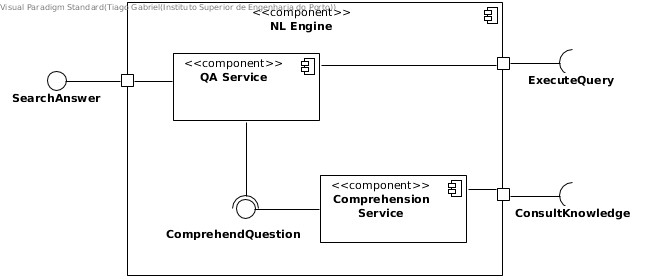
\includegraphics[width=\textwidth]{ch04/assets/nl-engine.jpg}
         \caption{Arquitetura detalhada do \textit{NL Engine}}
         \label{fig:nlengine_architecture}
     \end{subfigure}
\caption{Arquitetura do protótipo, apresentando um vista genérica e uma mais específica do componente \textit{NL Engine}}
\label{fig:prototype_architecture}
\end{figure}
%
\begin{itemize}
    \item 
    {
        \textit{NL Presentation} -- responsável pela interação com o utilizador. Integra a camada de apresentação do {\productname} e, como tal, é desenvolvido de acordo com as especificidades do subsistema em que se insere;
    }
    \item 
    {
        \textit{NL Engine} -- o módulo de linguagem natural, ou seja, o \inquotes{motor} que permite a tradução de linguagem natural em intenções e respetivas entidades. Integra a camada aplicacional de serviços do produto;
    }
    \item 
    {
        \textit{Q\&A Service} -- trata-se de um subcomponente o \textit{NL Engine}, que conhece as partes envolvidas no processo de aquisição de resposta, sendo responsável orquestrar esse processo. Trabalha em conjunto com o \textit{Comprehension Service} com o objetivo de identificar e mapear a intenção e entidades de uma dada \textit{query} de linguagem natural para obter a resposta da fonte de dados produtivos. Numa analogia à anatomia humana, pode ser considerado o \inquotes{cérebro} do processo;
    }
    \item 
    {
        \textit{Comprehension Service} -- outro subcomponente do \textit{NL Engine}, trabalha com a base de conhecimento definida (\textit{NL Knowledge Base}) para executar a tarefa de compreender a pergunta colocada. É neste componente que se insere a ferramenta para processamento de linguagem natural escolhida;
    }
    \item 
    {
        \textit{Feedback Management} -- tem a responsabilidade de gerir o \textit{feedback} providenciado pelo utilizador e disponibiliza serviços para a gestão dessa mesma informação, que incluem o desencadear do processo de aprendizagem, por exemplo. Inicialmente, o \textit{feedback} pode ser consultado manualmente, possibilitando o uso dessa informação para a melhoria do sistema. Contudo, podem ser aplicadas estratégias que façam uso desta informação de forma automática;
    }
    \item 
    {
        \textit{NL Knowledge Base} -- base de conhecimento de domínio, incluída na camada de persistência do {\productname}. É configurada pela equipa de desenvolvimento e deve mapear as entidades de domínio, as intenções em que estão envolvidas e suportar o registo de \textit{feedback}, para que possa ser usado na aprendizagem do módulo;
    }
    \item 
    {
        \textit{ProductionDB} -- armazém de dados de negócio. Contém a informação que o utilizador deseja obter através de linguagem natural.
    }
\end{itemize}

Apesar da elucidação acerca da responsabilidade de cada componente no sistema, é importante detalhar a forma como estes interagem entre si, para atingir o objetivo. A Figura~\ref{fig:prototype_sequence_diagram} mostra como se desenrola a comunicação entre os diversos componentes, que se passa a descrever: o utilizador (\textit{User}) questiona o sistema através da interface gráfica (\textit{NL Presentation}). A questão é encaminhada para o \textit{Q\&A Service} que se encarrega de \inquotes{pedir} ao \textit{Comprehension Service} para que lhe forneça a compreensão sob forma de representação intermediária. Posto isto, o \textit{Comprehension Service} consulta a base de conhecimento (\textit{NL Knowledge Base}) para consultar o conteúdo existente e, aplicando modelos de \gls{ml}, faz o reconhecimento das intenções e entidades presentes na questão. O \textit{Q\&A Service} trata de converter a representação numa linguagem compatível com o \textit{ProductionDB} e executa a \textit{query} gerada. Aquando a aquisição dos dados, o \textit{Q\&A Service} trata de \inquotes{documentá-los}, ou seja, colocar metadados que sejam importantes para processamento posterior. Por fim, a \textit{NL Presentation} processa o resultado para que este seja apresentado num formato adequado ao utilizador. Após o processo descrito, o sistema pede por \textit{feedback} do utilizador (\textit{User}). Aquando recebido, o \textit{feedback} é entregue ao \textit{Feedback Management}, que se encarrega de enviá-lo para a \textit{NL Knowledge Base} para que seja armazenado. Este último componente salva o \textit{feedback} terminando com sucesso o processo inteiro, estando o sistema pronto para inicializar um novo.

\begin{sidewaysfigure}
    \centering
    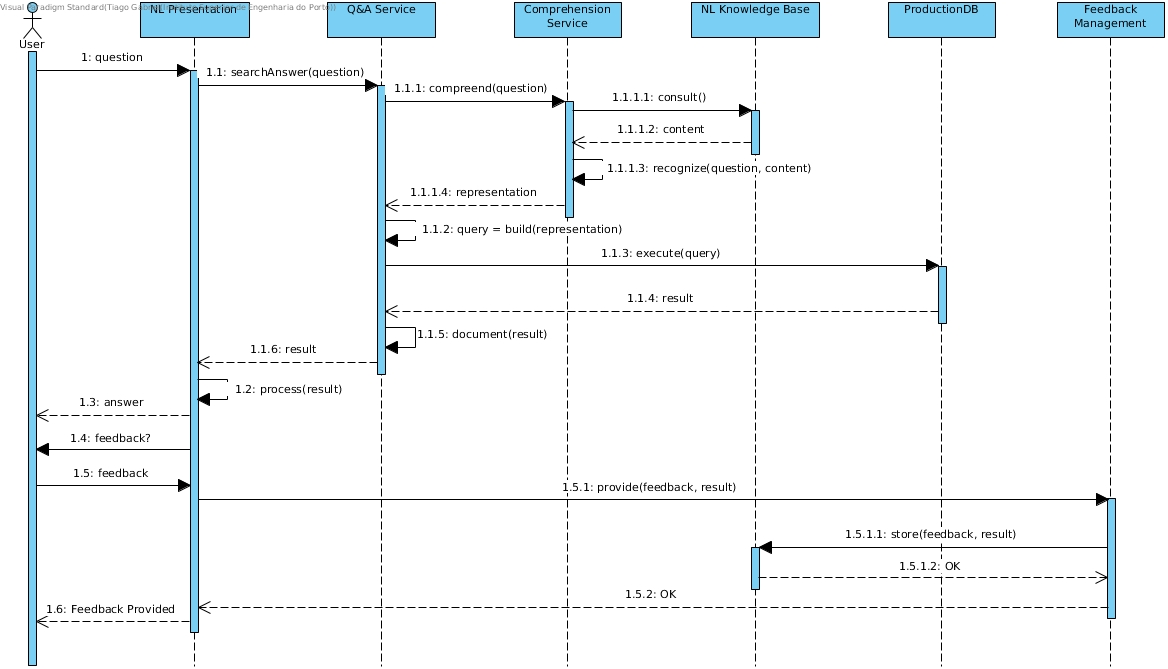
\includegraphics[width=\textwidth]{ch04/assets/workflow.jpg}
    \caption{Comunicação entre os componentes do módulo de linguagem natural}
    \label{fig:prototype_sequence_diagram}
\end{sidewaysfigure}

%%%%%%%%%%%%%%%%%%%%%%%%%%%%%%%%%
%           SECTION
%%%%%%%%%%%%%%%%%%%%%%%%%%%%%%%%%
\section{Síntese} 
\label{sec:chap04_chaptersummary}
Neste capítulo descreveu-se o processo que levou à especificação do modelo, dando ênfase aos detalhes da sua arquitetura. 

Começou-se por descrever a apreciação feita, em contexto prático, a algumas das ferramentas e abordagens anteriormente estudadas, fazendo referência aos seus pontos favoráveis e desfavoráveis. A conclusão retirada foi a de que a abordagem de reconhecimento de intenções e entidades seria a escolha adequada para o modelo a conceber.

Posteriormente, apresentou-se o modelo proposto para a solução de \gls{iln}, descrevendo a visão contemplada, as áreas funcionais -- \textit{Q\&A}, \textit{Feedback} e \textit{Knowledge Base} -- e os casos de uso identificados, detalhando os mais importantes. Finalmente, a arquitetura num ponto de vista lógica, explicando os componentes e o fluxo de trabalho entre eles, no qual se apresenta um cenário genérico do funcionamento do processo de tradução e \textit{feedback}.

\chapter{Desenvolvimento}
\label{chap:Chapter5}
\tbd

%%%%%%%%%%%%%%%%%%%%%%%%%%%%%%%%%
%           SECTION
%%%%%%%%%%%%%%%%%%%%%%%%%%%%%%%%%
\section{Processo de Configuração}
\label{sec:chap05_configprocess}
\tbd

\subsection{Intenções e Entidades}
\tbd

\subsection{Respostas Estáticas}
\tbd

\subsection{Integração dos Serviços}
\tbd

%%%%%%%%%%%%%%%%%%%%%%%%%%%%%%%%%
%           SECTION
%%%%%%%%%%%%%%%%%%%%%%%%%%%%%%%%%
\section{Implementação do Protótipo}
\label{sec:chap05_prototypeimplementation}
\tbd

\subsection{Especificação dos Componentes}
\tbd

\subsection{Fluxo Aplicacional}
\tbd

%%%%%%%%%%%%%%%%%%%%%%%%%%%%%%%%%
%           SECTION
%%%%%%%%%%%%%%%%%%%%%%%%%%%%%%%%%
\section{Síntese do Capítulo}
\label{sec:chap05_chaptersummary}
\chapter{Validação}
\label{chap:Chapter6}
\tbd

%%%%%%%%%%%%%%%%%%%%%%%%%%%%%%%%%
%           SECTION
%%%%%%%%%%%%%%%%%%%%%%%%%%%%%%%%%
\section{Resposta às Questões-Chave}
\label{sec:chap06_answers}
\tbd

%%%%%%%%%%%%%%%%%%%%%%%%%%%%%%%%%
%           SECTION
%%%%%%%%%%%%%%%%%%%%%%%%%%%%%%%%%
\section{Uso do \textit{Feedback}}
\label{sec:chap06_feedback_usage}
\tbd

%%%%%%%%%%%%%%%%%%%%%%%%%%%%%%%%%
%           SECTION
%%%%%%%%%%%%%%%%%%%%%%%%%%%%%%%%%
\section{Síntese do Capítulo}
\label{sec:chap06_chaptersummary}
\tbd

\chapter{Conclusões}
\label{chap:Chapter7}
Com o presente trabalho tentou-se contribuir para o conhecimento na área das \gls{iln}, através da conceção de um módulo de linguagem natural. Assim, é conveniente salientar as conclusões alcançadas, relacioná-las com os objetivos, criticar as suas limitações e referir as perspetivas futuras. Por isso, inicia-se por avaliar em que medida os objetivos foram cumpridos. Depois, especificam-se as contribuições e de que forma se apresentam como respostas para o problema. Finalmente, são constatadas as limitações do trabalho desenvolvido e perspetivas de trabalho futuro, apontando problemas em aberto ou as alternativas a contemplar.

%%%%%%%%%%%%%%%%%%%%%%%%%%%%%%%%%
%           SECTION
%%%%%%%%%%%%%%%%%%%%%%%%%%%%%%%%%
\section{Avaliação de Objetivos} 
\label{sec:chap07_goals_evaluation}
O trabalho descrito nesta tese consistiu na conceção de um módulo de linguagem natural, levando ao desenvolvimento de um protótipo que se demonstra capaz de compreender perguntas em formato textual, associadas ao domínio da manufatura, possibilitando a extração de informação das fontes de dados produtivos.

Na base da conceção do módulo e desenvolvimento do protótipo esteve um estudo teórico focado no \gls{pln}, mais especificamente das \gls{iln}, por forma conhecer o estado da arte desta área, nomeadamente para a compreensão de abordagens e seleção de ferramentas pertinentes para o trabalho. A abordagem adotada é fruto deste estudo, que não define nenhuma como sendo a ideal, mas sim aquela que melhor se enquadra na realidade do problema, oferecendo melhores contrapartidas. Assim, o modelo idealizado assenta sobre uma abordagem designada no âmbito desta tese por reconhecimento de intenções e entidades.

Para comprovar a validade do módulo concebido, realizaram-se testes focados na capacidade do protótipo compreender a linguagem natural de diferentes níveis e de dar resposta às questões colocadas, que visam a extração de conhecimento acerca de processos de fabrico. O protótipo respondeu adequadamente aos critérios de sucesso fixados, pelo que é legítimo concluir que os objetivos propostos foram atingidos.
% Face aos objetivos definidos (ver Secção~\ref{sec:chap01_objectives}), que englobam a conceção de um módulo, para interface com o {\productname} e o desenvolvimento de um protótipo capaz de compreender linguagem natural, conclui-se que o trabalho cumpriu-os, face ao critérios de sucesso apontados (ver Secção~\ref{sec:chap01_solutionevaluation}).

% O desenvolvimento do protótipo e a sua validação levaram a perceber que o modelo idealizado permite, de facto, a compreensão da linguagem natural textual e a extração de conhecimento relativo a processos de fabrico, sendo possível a sua aplicabilidade num contexto industrial.

%%%%%%%%%%%%%%%%%%%%%%%%%%%%%%%%%
%           SECTION
%%%%%%%%%%%%%%%%%%%%%%%%%%%%%%%%%
\section{Resposta ao Problema} 
\label{sec:chap07_problem_response}
O trabalho concretizado advém do pressuposto que o uso de linguagem natural no contexto do {\productname} pode melhorar a usabilidade do sistema e consequentemente, simplificar o processo de apoio à decisão dos seus clientes. Nesse sentido, tiveram-se como objetivos a conceção de um módulo de linguagem natural e desenvolvimento de um protótipo, aplicando o modelo idealizado.

Ainda que se demonstre que o módulo concetualizado permite a compreensão da linguagem natural e a resposta a questões-chave no processo de fabrico, nada se pode concluir acerca do seu impacto na usabilidade ou no processo de decisão, dado à natureza da solução desenvolvida, sendo ela um protótipo.

O trabalho atende à resolução do problema através da idealização de um módulo de linguagem natural, cuja aplicação prática se prova eficaz, ainda que de forma limitada. A especificação deste módulo, bem como o desenvolvimento do protótipo servem de base para a integração de \glspl{iln} no contexto do {\productname}.

%%%%%%%%%%%%%%%%%%%%%%%%%%%%%%%%%
%           SECTION
%%%%%%%%%%%%%%%%%%%%%%%%%%%%%%%%%
\section{Limitações e Trabalho Futuro} 
\label{sec:chap07_future_work_limitations}
Dificilmente se pode considerar um trabalho neste contexto, ou em muitos outros, como acabado. Este trabalho tem algumas limitações, que ao serem identificadas, possibilitam a introdução de novas ideias e desafios. Por conseguinte, apresentam-se algumas das limitações encontradas, sugerindo formas das ultrapassar, sempre que possível, e também algumas indicações de trabalho futuro:

\begin{itemize}
    \item 
    {
        Uma das grandes limitações do protótipo é não fazer uso da capacidade de interação com o utilizador para obter \textit{feedback} sobre as respostas dadas, usando-o para melhorar a previsão das intenções. Nesse sentido, a inclusão de um novo componente na arquitetura proposta, para a gestão do \textit{feedback}, poderia contribuir para a robustez da fase de compreensão de linguagem natural;
    }
    \item
    {
        Ainda que o protótipo esteja preparado para a integração de novas fonte de dados, o processo de transformação da representação intermediária para a linguagem específica dessa fonte pode ser uma tarefa complexa e morosa, \exempligratia{a conversão de representação intermediária para \gls{sql}}. Posto isto, o constituição de uma camada de abstração (\inquotes{fachada}) para o acesso a essas fontes de dados, pelo uso de ferramentas como o GraphQL ou no contexto da Web Semântica, pode contribuir para o acesso mais simples a novas fontes de dados;
    }
    \item
    {
        Apesar do protótipo ser capaz de tratar entidades temporais, apenas o faz para os meses, ou seja, exclui datas e horas específicas ou outras variações. O Microsoft LUIS produz os metadados necessários para a transformação, pelo que é adequada a implementação de estratégias para a normalização das datas, com intuito de serem usadas no carregamento de dados;
    }
    \item
    {
        Para usar o protótipo é necessário o acesso à Internet, ou seja, não há mecanismo que possibilite o seu uso sem acesso à rede. Nesse sentido, uma das sugestões é a adaptação do modelo idealizado para o desenvolvimento de uma solução interna, usando as ferramentas estudadas. Assim, há a necessidade de aprofundar o conhecimento delas e em que medida podem ser aplicadas com o modelo concebido;
    }
    \item
    {
        A solução desenvolvida não é genérica o suficiente para se adaptar a diferentes domínios, uma vez que parte do modelo de dados deve constar na base de conhecimento. Para isto, requer-se um estudo mais aprofundado da área de \gls{ia} aplicada à linguagem natural ou às \glspl{iln};
    }
    \item
    {
        Para dar resposta a perguntas multidimensionais, o protótipo classifica as entidades da frase com base na sua posição na frase, sendo então necessário que o modelo \gls{ml} esteja treinado para esse efeito. Mas, pressupõe-se que a introdução de um \inquotes{fluxo de conversação} possa simplificar este processo, na medida em que se introduz o fator \inquotes{contexto}, quebrando o nível multidimensional em vários níveis unidimensionais, permitindo ao utilizador indicar o que pretende, passo a passo; 
    }
    \item 
    {
        O uso de outras línguas para além do inglês, no contexto deste protótipo, obrigariam a redefinir uma nova base de conhecimento para cada língua nova a adicionar. No entanto, e caso seja um requisito relevante, pode-se realizar um estudo que leve a concluir acerca das estratégias existentes e qual apresenta mais e melhores benefícios para uma solução final, adaptando o modelo para tal;
    }
    \item 
    {
        O protótipo não pode ser transposto diretamente para uma solução interna, devido à sua natureza. Por isso, de acordo com a ferramenta que seja escolhida para o efeito, propõe-se que esse processo de escolha leve também em consideração o esforço necessário para a transição, pelo que, das ferramentas estudadas, supõe-se que Rasa apresenta melhores contrapartidas.
    }
\end{itemize}

Como  se  pode  constatar, há  ainda  imenso  trabalho  a  fazer, englobando desenvolvimento e mais pesquisa. No entanto, isso significa novos desafios e caminhos a percorrer, permitindo que este trabalho evolua, originando uma (primeira) \gls{iln} no contexto \gls{mes}, o que significa mais um passo para a Indústria 4.0.

%----------------------------------------------------------------------------------------
%	BIBLIOGRAPHY
%----------------------------------------------------------------------------------------

\printbibliography[heading=bibintoc]

%----------------------------------------------------------------------------------------
%	THESIS CONTENT - APPENDICES
%----------------------------------------------------------------------------------------

\appendix % Cue to tell LaTeX that the following "chapters" are Appendices

% Include the appendices of the thesis as separate files from the Appendices folder
% Uncomment the lines as you write the Appendices

\chapter{Plano de Trabalho Previsto}
\label{AppendixA}
Neste apêndice presenta-se o plano de trabalho definido inicialmente para o projeto.

\begin{figure}[!ht]
    \centering
    \rotatebox{90}{
        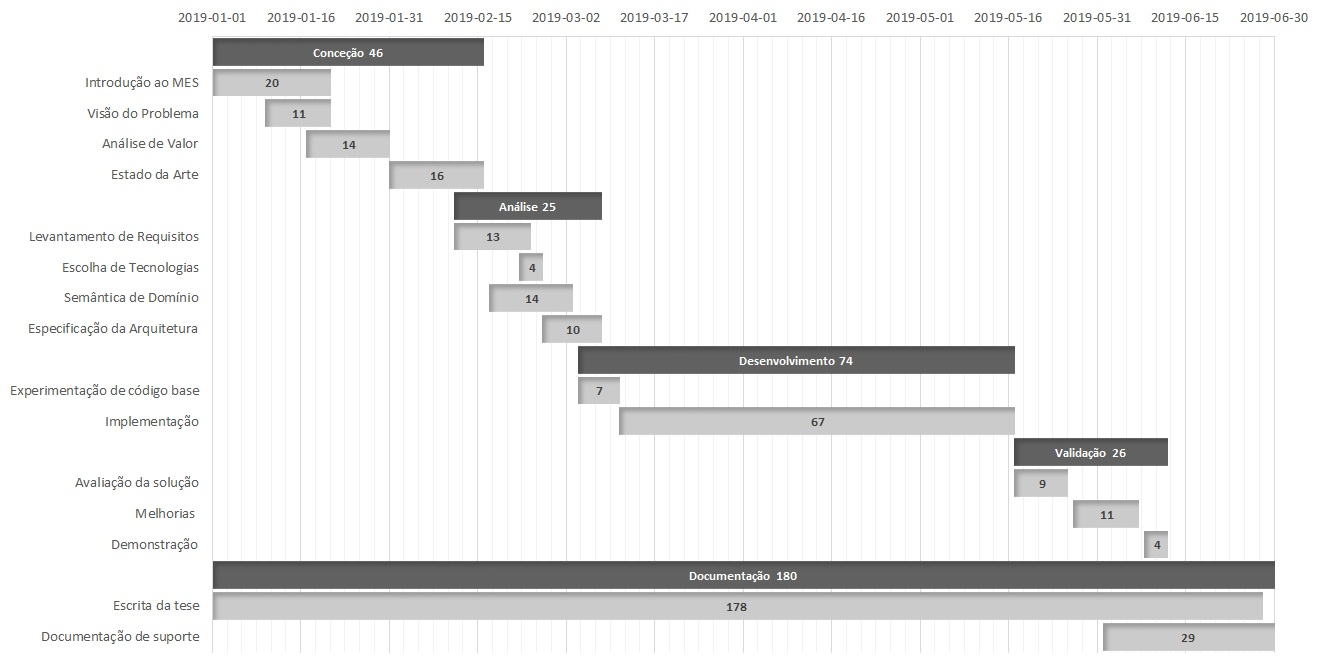
\includegraphics[width=\textwidth]{appendices/assets/gantt.jpg}
    }
    \caption{Diagrama de \textit{Gantt} referente ao planeamento do projeto}
\end{figure}

\chapter{Análise de Valor}
\label{AppendixB}
Esta capítulo visa a análise da oportunidade de negócio que surge com a nova funcionalidade, cuja abordagem é explorada neste trabalho.

\section{O Processo de Inovação}
De acordo com~\textcite{ffe_effectivemethods_tools_techniques}, o processo de inovação, representado na Figura~\ref{fig:inovation_process}, está dividido em três áreas -- o \gls{ffe}, \gls{npd} e a comercialização -- que correspondem às fases inerentes ao \gls{ncd}, um modelo desenvolvido por um conjunto de empresas, com o objetivo de \inquotes{[...]~fornecer uma linguagem e compreensão comum para as atividades \textit{front end}}\footnote{Tradução livre de autor. No original \inquotes{[...]~to provide a common language and insights on the front end activities.}.}~\parencite{providing_clarity_common_language_ffe}.

O \gls{ffe} representa uma oportunidade para melhoria de todo o processo de inovação, focando todas as atividades que antecedem o desenvolvimento do produto, com o propósito de potenciar o valor, a importância e a probabilidade de sucesso das fases que se seguem. Ou seja, consiste no investimento do tempo em atividades de discussão da ideia, por forma a identificar e estruturar o problema ou oportunidade~\parencite{ffe_effectivemethods_tools_techniques, ffe_theoretical_model}. Porém, as atividades inerentes ao \gls{ffe} são fundamentalmente diferentes da fase \gls{npd}, pelo que se torna necessária a definição de vocabulário específico, permitindo a geração de conhecimento e clara distinção entre as diferentes fases do processo~\parencite{ffe_effectivemethods_tools_techniques}.

\begin{figure}[!ht]
    \centering
    \includegraphics[width=.95\textwidth]{appendices/assets/inovation_process.jpg}
    \caption{O processo de inovação, extraído de~\textcite{ffe_effectivemethods_tools_techniques}}
    \label{fig:inovation_process}
\end{figure}

O modelo \gls{ncd}, demonstrado na Figura~\ref{fig:ncd_model}, baseado num modelo relacional ao invés de um processo linear, visa providenciar uma terminologia para o \gls{ffe}~\parencite{ffe_effectivemethods_tools_techniques}. A área interna define os cinco elementos chave do \textit{Front End of Inovation}: a identificação de oportunidade (\textit{Opportunity Identification}), a análise de oportunidade (\textit{Opportunity Analysis}), a geração e enriquecimento de ideias (\textit{Idea Generation and Enrichment}), a seleção de ideias (\textit{Idea Selection}) e a definição do conceito (\textit{Concept Definition}). O motor central (\textit{Engine}) corresponde à liderança, cultura e estratégia organizacional, que suporta os elementos que compõem o \gls{ffe}, são controláveis pela organização e possibilita a interação entre eles. Já na periferia, encontram-se os fatores de influência (\textit{Influencing Factors}), geralmente incontroláveis pela organização, consistem nas capacidades organizacionais, na estratégia de negócio, no mundo exterior, nomeadamente os canais de distribuição, clientes, fornecedores, concorrentes, política governamental ou legislação, ou quaisquer fatores que possam influenciar todo o processo de inovação~\parencite{ffe_effectivemethods_tools_techniques, providing_clarity_common_language_ffe}.

\begin{figure}[!ht]
    \centering
    \includegraphics[width=.55\textwidth]{appendices/assets/ncd_model.jpg}
    \caption{A representação do modelo \glsfirst{ncd}, extraído de~\textcite{ffe_effectivemethods_tools_techniques}}
    \label{fig:ncd_model}
\end{figure}

Quanto à representação do modelo, as partes internas são designadas de elementos por oposição a processos, pois estes implicam estrutura, que pode não ser possível ser aplicada. O formato circular indica que é esperado que as ideias fluam, circulem e iterem ao longo dos elementos, por qualquer ordem ou combinação, permitindo o uso dos elementos, repetidamente. Este comportamento é intrínseco às atividades do \gls{ffe}, permitindo uma definição clara do mercado, dos requisitos, dos riscos associados e do plano de negócio, tornando mais eficazes as fases de desenvolvimento e comercialização, devido à redução do tempo total de projeto, fruto da diminuição da repetição de algumas atividades~\parencite{ffe_effectivemethods_tools_techniques}. 

\section{O \textit{Fuzzy Front End} de Inovação}
Como mencionado anteriormente, o \gls{ffe} corresponde a um conjunto de atividades geralmente caóticas, imprevisíveis e não estruturadas que antecedem o desenvolvimento de um produto~\parencite{ffe_incremental_platform_breakthrough_products}. Todavia, é preciso perceber a natureza do produto a desenvolver, de forma a melhor enquadrar o processo de inovação.

Segundo~\textcite{ffe_incremental_platform_breakthrough_products}, pode-se caracterizar os produtos de acordo com a extensão da mudança ou do processo: incremental, requer pouca mudança a nível do produto ou do processo, uma vez que geralmente consiste na redução de custos, melhoria, extensão ou reposicionamento no mercado de produtos já existentes; plataforma, estabelecem uma arquitetura básica para uma nova geração de produtos ou processos; pioneiro, envolve uma mudança significativa no processo ou produto.

O presente trabalho visa o desenvolvimento dum módulo de linguagem natural para o {\productname}, uma plataforma já estabelecida, ou seja, trata-se de uma extensão ao produto já existente, enquadrando-se no tipo incremental. A ideia surge do processo de planeamento estratégico da empresa com a finalidade de trazer novas funcionalidades aos seus clientes, melhorando a qualidade do produto. Portanto, nas secções seguintes, aplica-se a metodologia explicitada, no sentido de enriquecer a proposta de projeto apresentada pela {\companyname}.

\subsection{Identificação da Oportunidade}
O \gls{pln} é uma área de investigação que explora a forma como os computadores podem manipular a linguagem natural (texto ou voz) para executar determinadas tarefas. Aplica-se em diversos campos de estudo: tradução, processamento de texto, interfaces com o utilizador, reconhecimento de voz, sistemas periciais~\parencite{nlp}.

\textcite{end_to_end_neural_nli_databases} menciona que, apesar da expressividade da \gls{sql}, os utilizadores necessitam de algum conhecimento técnico para perceber como extrair informação de um sistema, o que conduziu à investigação para o desenvolvimento de interfaces alternativas que permitam aos utilizadores, sem conhecimento técnico, explorar e interagir com os dados, de forma conveniente. Também \textcite{towards_theory_nli_databases} menciona que a necessidade de interfaces de linguagem natural se torna mais evidente, devido ao número de pessoas sem conhecimentos técnicos que acedem a informação através de \textit{browsers} ou telemóveis, tornando paradigmas como o reconhecimento de voz mais atrativos.

Nesse sentido, a {\companyname} tenciona o desenvolvimento do módulo de linguagem natural para que os utilizadores do produto, sem conhecimento orientado às tecnologias de informação, possam fácil, rápida e intuitivamente consultar o sistema. Desta forma, a funcionalidade destaca o produto pelo uso de novas tecnologias, facilita-se a interação com o sistema, reduzindo-se o tempo de formação técnica associado ao mesmo. 

\subsection{Análise da Oportunidade}
A pesquisa realizada por~\textcite{roadmap_nlp_research_is}, apresentada na Figura~\ref{fig:number_articles_per_year_nlp}, cuja metodologia consistiu na pesquisa de termos como \inquotes{Natural Language Processing} e \inquotes{NLP} em bases de dados académicas, determina que há uma tendência crescente de interesse por esta área. Nos últimos anos, a quantidade de dados textuais disponíveis nas redes sociais ou em sistemas de comunicação, juntamente com a necessidade de acesso a informação, contribuíram para o avanço e adoção comercial do \gls{pln}~\parencite{roadmap_nlp_research_is}.

\begin{figure}[!ht]
    \centering
    \includegraphics[width=.9\textwidth]{appendices/assets/number_articles_nlp.jpg}
    \caption{Número de artigos de \glsfirst{pln} pesquisados por ano, extraído de~\textcite{roadmap_nlp_research_is}}
    \label{fig:number_articles_per_year_nlp}
\end{figure}

Quanto ao segmento de mercado no qual se integra, cresce a visão de fábricas inteligentes, associadas à quarta revolução industrial, prezando a integração do operador humano num ambiente complexo e rico em dados~\parencite{social_factory}. \textcite{industry40_revolution_future_mes} afirma que a revolução supracitada é já conhecida pelas empresas, o que lhe permite tomar ações no sentido de definir o seu modelo de fabrico e o seu plano de transformação, particularmente na adaptação do \gls{mes} de forma a manter o desempenho, qualidade e agilidade nas desafios espoletados pelas empresas de manufatura. Portanto, a interação entre o ser humano e o sistema pode melhorar o processo de fabrico e potenciar o negócio, na medida em que o operador, em vez do trabalho manual repetitivo que pode facilmente ser automatizado, passa a tomar decisões no processo para resolução de problemas, as quais requerem acesso à informação correta e de forma atempada~\parencite{social_factory}. É nesse sentido que o {\productname} ganha vantagem com o desenvolvimento desta nova funcionalidade.

\subsection{Geração, Enriquecimento e Seleção de Ideias}
No seguimento deste assunto, foram realizadas duas reuniões com o supervisor do projeto na {\companyname}, em que foram discutidos alguns requisitos operacionais e de usabilidade, restrições ao desenvolvimento da solução, como a preferência por uso de ferramentas de \gls{pln} que possam ser mantidas internamente e a sua facilidade de utilização, e ideias para futuras implementações, as quais podem ter um impacto na especificação arquitetural do protótipo.

\begin{figure}
    \centering
    \resizebox{\textwidth}{!}{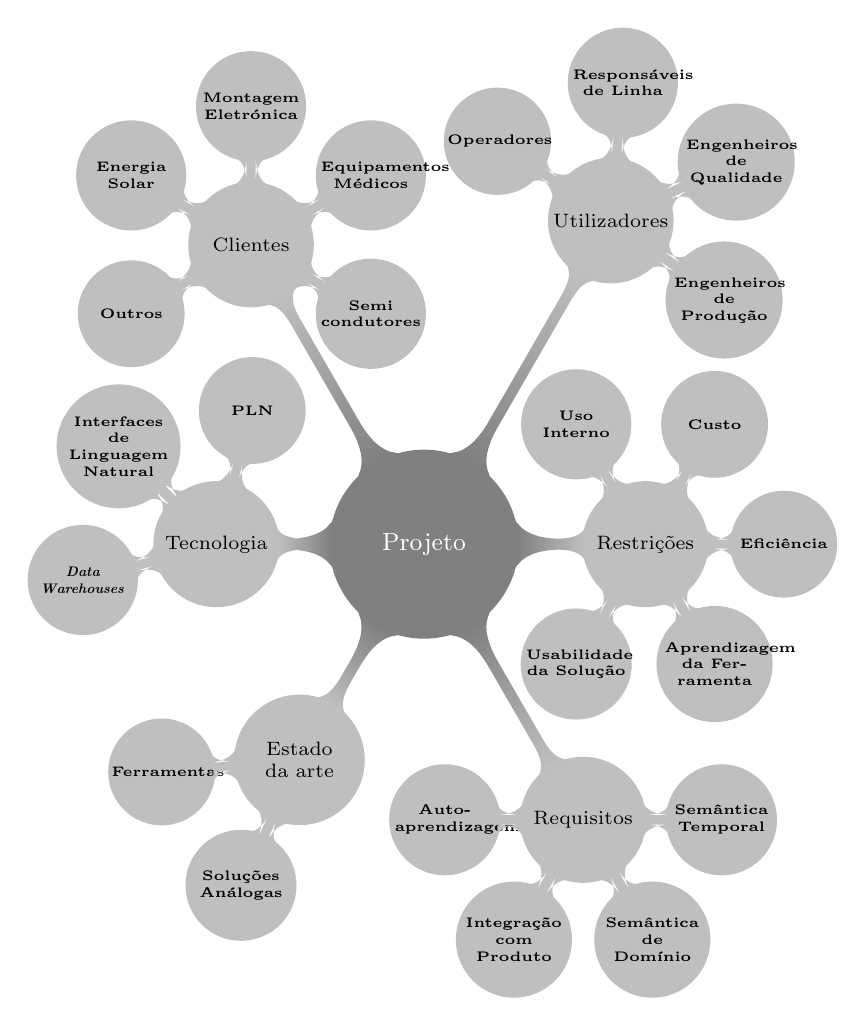
\begin{tikzpicture}
  \path[mindmap, concept color=black!50,text=white,
    every node/.append style={concept, minimum size=0.5cm, inner sep=0.2mm},
    level 1 concept/.append style={text width=1.5cm,font=\scriptsize},
    level 2 concept/.append style={text width=1.27cm,font=\tiny\bfseries,level distance=50}
  ]
    % Root
    node[text width=2.3cm,font=\small] {Projeto}
    %
    [clockwise from=0]
    child[concept color=black!25,text=black,level distance=80] { node {Restrições}
      [clockwise from=120]
      child { node {Uso Interno} }
      child { node {Custo} }
      child { node {Eficiência} }
      child { node {Aprendizagem da Ferramenta} }
      child { node {Usabilidade da Solução} }
    }
    %
    child[concept color=black!25,text=black,level distance=115] { node {Requisitos}
      [clockwise from=0]
      child { node {Semântica Temporal} }
      child { node {Semântica de Domínio} }
      child { node {Integração com Produto} }
      child { node {Auto-aprendizagem} }
    }
    %
    child[concept color=black!25,text=black,level distance=90] { node {Estado da arte} 
      [clockwise from=-115]
      child { node {Soluções Análogas} }
      child { node {Ferramentas} }
    }
    %
    child[concept color=black!25,text=black,level distance=75] { node {Tecnologia}
      [counterclockwise from=75]
      child { node {PLN} }
      child { node {Interfaces de Linguagem Natural} }
      child { node {\textit{Data Warehouses}} }
    }
    %
    child[concept color=black!25,text=black,level distance=125] { node {Clientes}
      [counterclockwise from=-30]
      child { node {Semi\\condutores} }
      child { node {Equipamentos Médicos} }
      child { node {Montagem Eletrónica} }
      child { node {Energia Solar} }
      child { node {Outros} }
    }
    child[concept color=black!25,text=black,level distance=135] { node {Utilizadores}
      [counterclockwise from=-35]
      child { node {Engenheiros de Produção} }
      child { node {Engenheiros de Qualidade} }
      child { node {Responsáveis de Linha} }
      child { node {Operadores} }
    };
\end{tikzpicture}}
    \caption{\textit{Mindmap} das ideias e conceitos gerados}
    \label{fig:mindmap}
\end{figure}

Em relação às ideias e conceitos contempladas no \textit{mindmap} da Figura~\ref{fig:mindmap}, o presente projeto pretende dar resposta a praticamente todos, tendo em consideração que, numa fase inicial, o cumprimento de todos é praticamente inatingível. A descrição de cada conceito é feito de seguida:

\begin{itemize}
    \item
    {
        \textit{Tecnologia} -- a ideia inerente ao trabalho assenta sobre as temáticas de \gls{pln}, especificamente Interfaces de Linguagem Natural, e \textit{Data Warehouses}. Esta consiste no estudo aprofundado deste tipo de interfaces orientado à consulta em armazéns de dados e disseminação do conhecimento internamente, para que no futuro, o projeto possa ter continuidade;
    }
    \item
    {
        \textit{Estado da Arte} -- abordagem de ferramentas e soluções análogas, com o objetivo de especificar uma arquitetura para o sistema. Este processo dá origem aos documentos de especificação que devem ser usados para consulta por parte dos desenvolvedores, quer numa perspetiva de conhecimento arquitetural, quer das ferramentas que são usadas;
    }
    \item
    {
        \textit{Clientes} -- uma vez que a {\companyname} possui clientes com diferentes realidades, a ideia é que o módulo final esteja preparado para elaborar consultas em qualquer domínio, de forma configurada ou cerne da solução. Contudo, como já abordado anteriormente, no contexto deste trabalho, apenas um domínio será considerado;
    }
    \item
    {
        \textit{Utilizadores} -- a solução deverá responder às necessidades de qualquer utilizador, desde os mais técnicos (Engenheiros de Produção) aos menos técnicos (Operadores). Porém, o protótipo terá em consideração os utilizadores mais comuns do {\productname};
    }
    \item
    {
        \textit{Restrições} -- nesta temática, foram discutidas alternativas como a avaliação do custo de uma ferramenta proprietária, uso de ferramentas \textit{open source} ou o desenvolvimento interno da própria biblioteca de \gls{pln}, de modo a garantir que não existem dependências externas à plataforma. Também foram discutidas a eficiência da solução em contexto produtivo, a facilidade de aprendizagem e usabilidade da mesma. Assim, a usabilidade do módulo de linguagem natural será estudada a partir do mecanismo de \textit{feedback} provido na solução e através de inquéritos aos utilizadores, o que também se aplica para a aprendizagem da ferramenta. Relativamente aos restantes tópicos, não houve conclusão acerca das ideias a serem selecionadas;
    }
    \item
    {
        \textit{Requisitos} -- pressupõe-se o uso de auto-aprendizagem para adaptação automática do módulo ao \textit{feedback} do utilizador, ainda que para o protótipo, a resposta a uma simples pergunta como \inquotes{A resposta obtida foi-lhe útil?} é suficiente. Também a integração com o produto, quer a nível aplicacional, quer a nível de processo deve ser considerada, o que resultará na organização de \textit{meetups} com as equipas responsáveis pelo processo de manutenção da plataforma. Quanto aos restantes conceitos, não houve conclusão acerca das ideias selecionadas.
    }
\end{itemize}

\subsection{Definição do Conceito}
Todo o processo presente no modelo \gls{ncd} de \gls{ffe} culmina com a definição do conceito, a fase que encaminha o projeto para a implementação~\parencite{ffe_effectivemethods_tools_techniques}.

O presente trabalho, denominado de \inquotes{Natural Language Querying} consiste no desenvolvimento de um protótipo de um módulo de linguagem natural e definição de uma abordagem que será tida em conta no módulo final para interface com o {\productname}. Esse módulo final permitirá a consulta e pesquisa de estados do processo de fabrico por utilizadores com pouco ou nenhum conhecimento associado a tecnologias de informação, garantindo a interação com o sistema de uma forma simples, fácil e intuitiva, melhorando o processo numa perspetiva de apoio à decisão (ver Secção~\ref{sec:chap01_problem}). Os objetivos deste projeto estão descritos na Secção~\ref{sec:chap01_objectives}, a metodologia e critérios de sucesso na Secção~\ref{sec:chap01_solutionevaluation}, e o respetivo plano de trabalho no Capítulo~\ref{sec:chap01_workmethodology}.

O projeto traz benefícios para a empresa e o seu produto, pelo estudo e adoção de tecnologia de \gls{pln} num contexto industrial, pela possível melhoria de usabilidade do sistema e pela evolução no processo de apoio à decisão dos seus clientes. Uma vez que o {\productname} é um produto bem posicionado no mercado, não se esperam riscos a nível comercial. Contudo, a uso de tecnologia recente, cujos conceitos não estão totalmente estudados e cujos trabalhos de investigação são limitados, pode provocar atrasos no desenvolvimento do projeto ou incumprimento do orçamento definido. Não obstante, o projeto avança com o desenvolvimento de um protótipo, fase que decidirá a inclusão do módulo na plataforma da {\companyname}.


\chapter{Protótipo}
\label{AppendixC}
Neste apêndice são mostrados alguns artefactos recolhidos ao longo das fases de conceção, desenvolvimento e validação do protótipo.

\section{Configuração}
Nesta secção apresentam-se algumas imagens referentes ao processo de configuração levado no protótipo.
%
\begin{figure}[!ht]
    \centering
    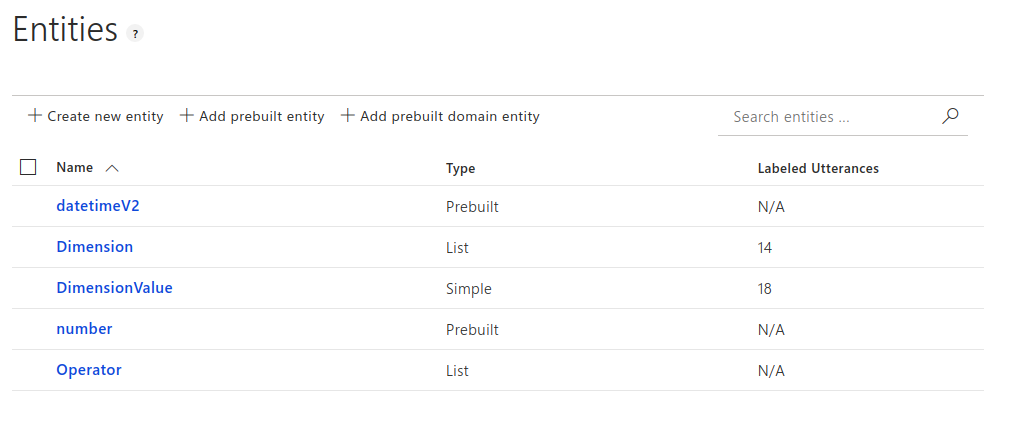
\includegraphics[width=\textwidth]{appendices/assets/kb07.png}
    \caption{Definição das entidades esperadas}
\end{figure}
%
\begin{figure}
\centering
    \begin{subfigure}{.9\textwidth}
        \centering
        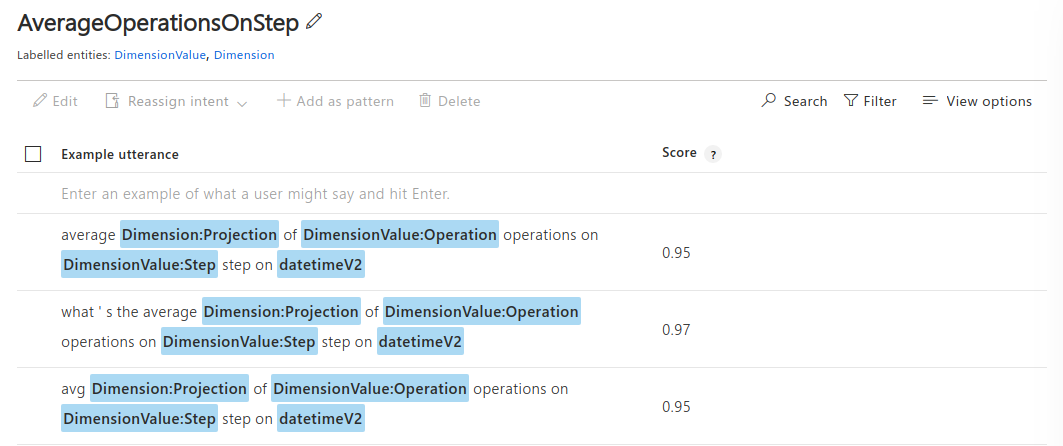
\includegraphics[width=\textwidth]{appendices/assets/kb01.png}
        \caption{Intenção \textit{AverageOperationOnStep}}
     \end{subfigure}
     \begin{subfigure}{.9\textwidth}
         \centering
        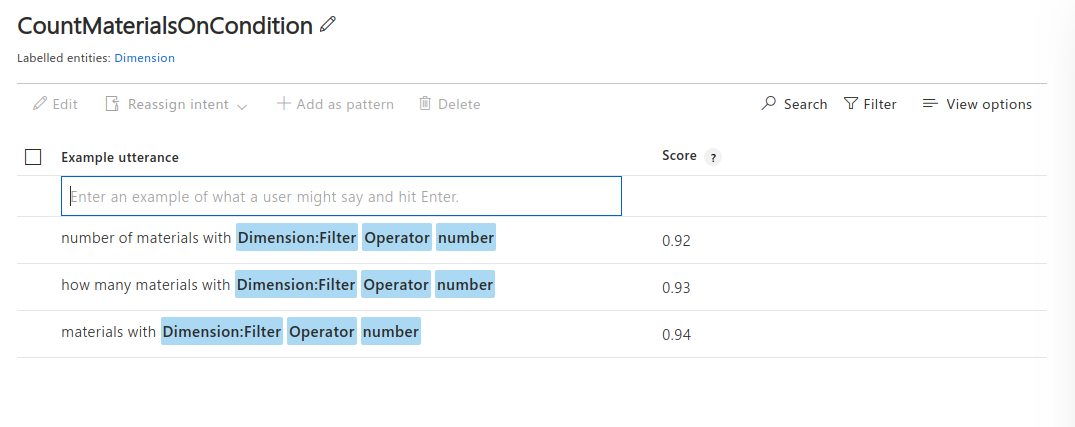
\includegraphics[width=\textwidth]{appendices/assets/kb02.png}
        \caption{Intenção \textit{CountMaterialsOnCondition}}
     \end{subfigure}
     \begin{subfigure}{.9\textwidth}
        \centering
        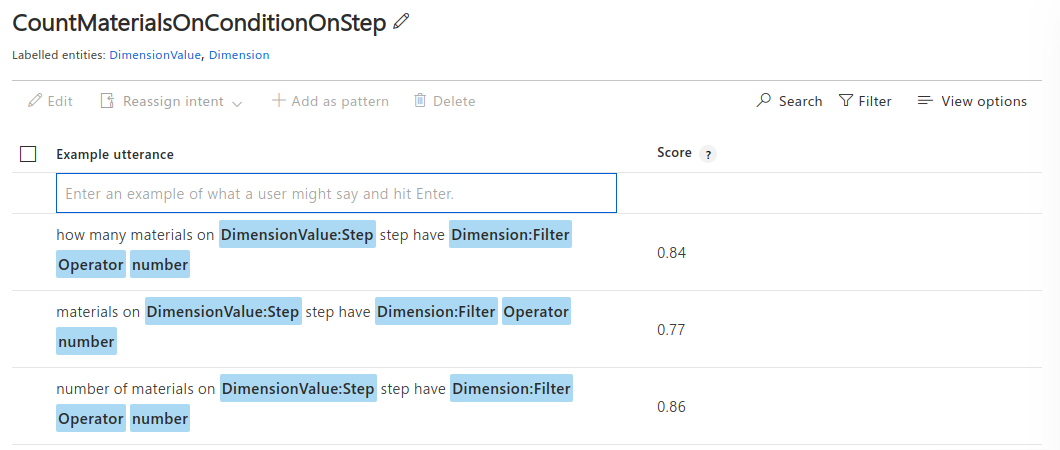
\includegraphics[width=\textwidth]{appendices/assets/kb03.png}
        \caption{Intenção \textit{CountMaterialsOnConditionOnStep}}
     \end{subfigure}
\caption{Intenções definidas, contendo as expressões e respetivas entidades}
\end{figure}
%
\begin{figure}
    \centering
         \begin{subfigure}{.9\textwidth}
        \centering
        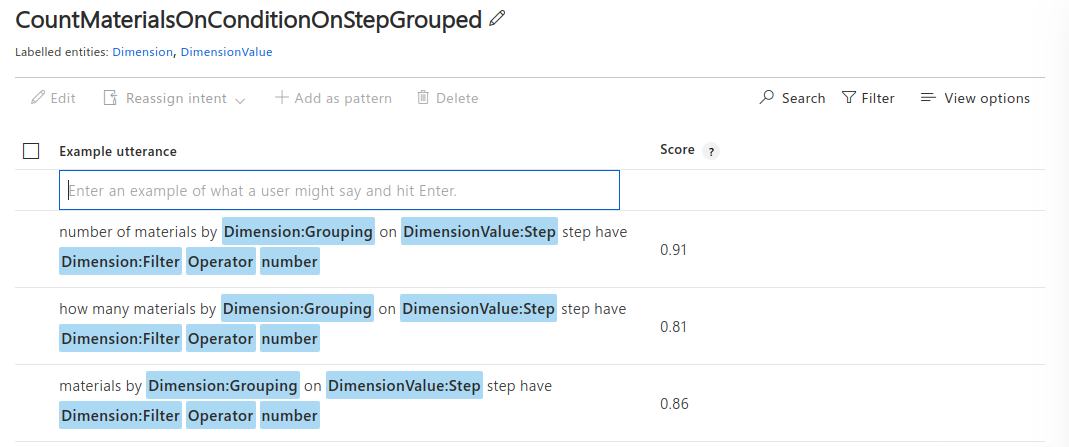
\includegraphics[width=\textwidth]{appendices/assets/kb04.png}
        \caption{Intenção \textit{CountMaterialsOnConditionOnStepGrouped}}
     \end{subfigure}
     \begin{subfigure}{.9\textwidth}
        \centering
        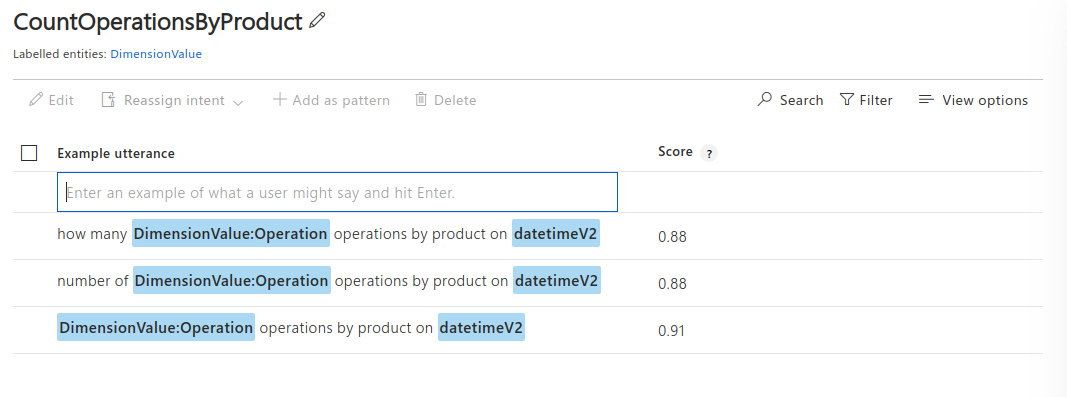
\includegraphics[width=\textwidth]{appendices/assets/kb05.png}
        \caption{Intenção \textit{CountOperationsByProduct}}
     \end{subfigure}
     \begin{subfigure}{.9\textwidth}
        \centering
        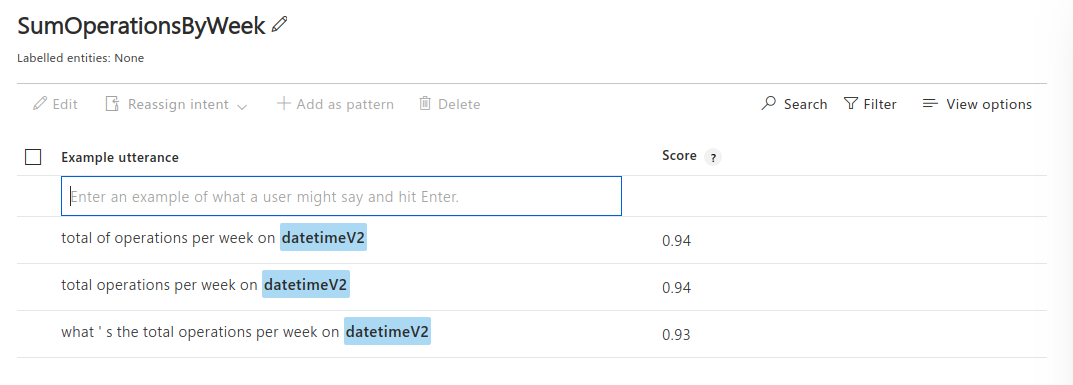
\includegraphics[width=\textwidth]{appendices/assets/kb06.png}
        \caption{Intenção \textit{SumOperationsByWeek}}
     \end{subfigure}
    \caption{Continuação das intenções definidas, contendo as expressões e respetivas entidades}
\end{figure}

\clearpage

\section{Validação}
Nesta secção apresentam-se algumas imagens referentes ao processo de validação do protótipo.

\begin{figure}[!ht]
\centering
    \begin{subfigure}{.48\textwidth}
        \centering
        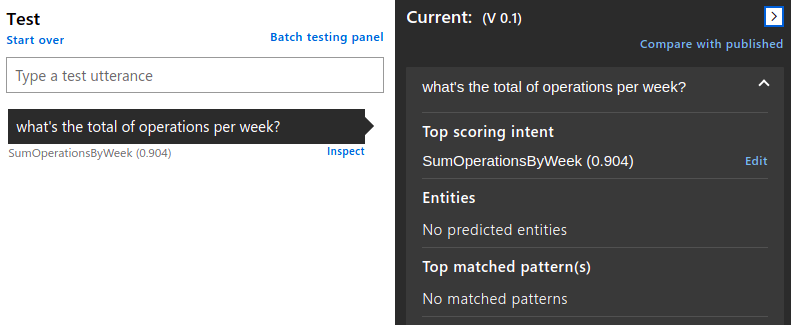
\includegraphics[width=\textwidth]{appendices/assets/nlcomprehension01.png}
        \caption{Intenção \textit{SumOperationsByWeek}}
     \end{subfigure}
     \begin{subfigure}{.48\textwidth}
         \centering
        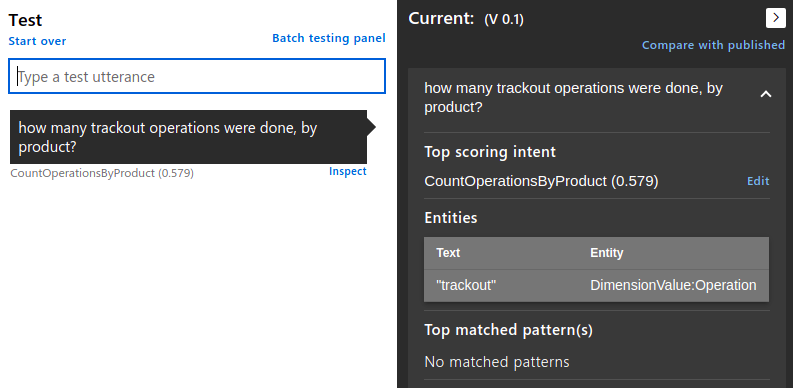
\includegraphics[width=\textwidth]{appendices/assets/nlcomprehension02.png}
        \caption{Intenção \textit{CountOperationByProduct}}
     \end{subfigure}
     \bigbreak
     \begin{subfigure}{.48\textwidth}
        \centering
        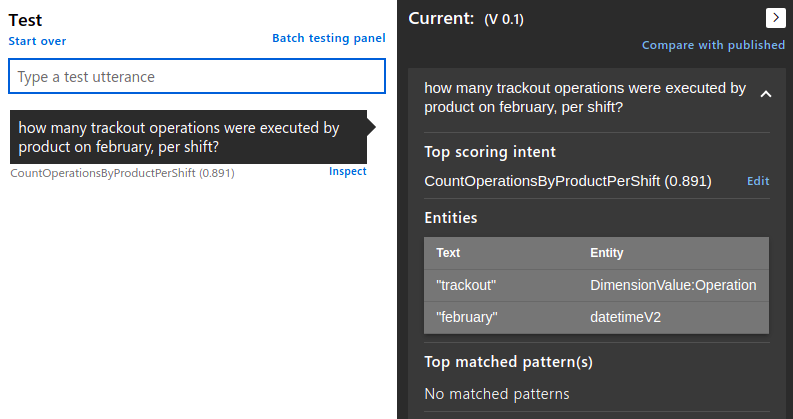
\includegraphics[width=\textwidth]{appendices/assets/nlcomprehension03.png}
        \caption{Intenção \textit{AverageOperationsOnStep}}
     \end{subfigure}
     \begin{subfigure}{.48\textwidth}
        \centering
        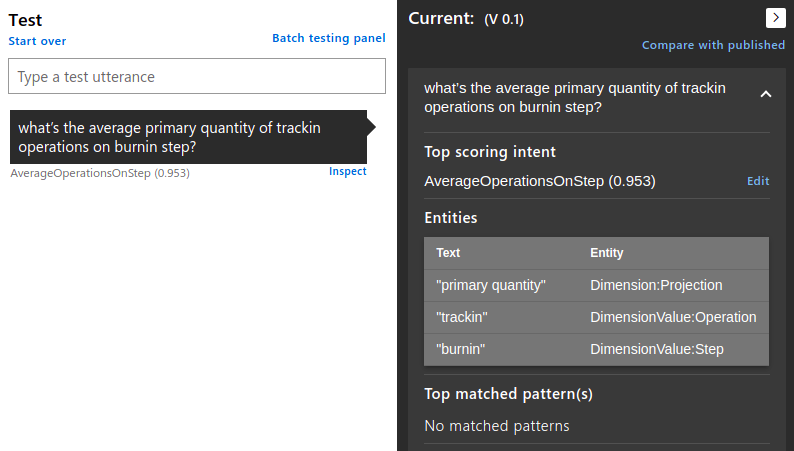
\includegraphics[width=\textwidth]{appendices/assets/nlcomprehension04.png}
        \caption{Intenção \textit{CountOperationsOnConditionOnStepGrouped}}
     \end{subfigure}
     \bigbreak
     \begin{subfigure}{.48\textwidth}
        \centering
        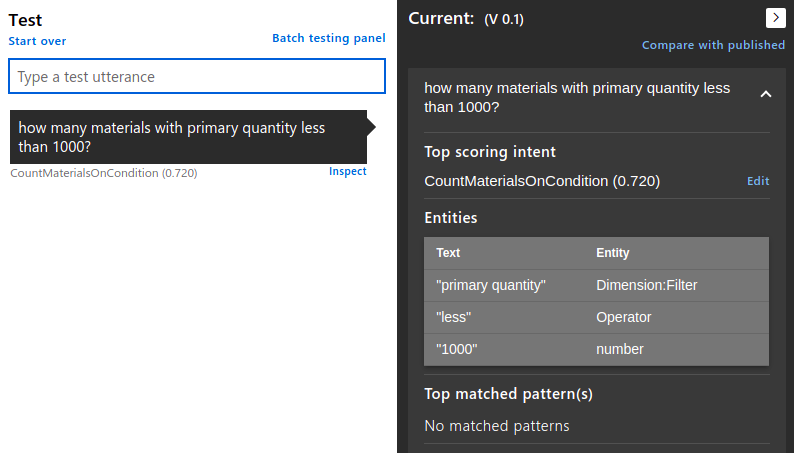
\includegraphics[width=\textwidth]{appendices/assets/nlcomprehension05.png}
        \caption{Intenção \textit{AverageOperationsOnStep}}
     \end{subfigure}
     \begin{subfigure}{.48\textwidth}
        \centering
        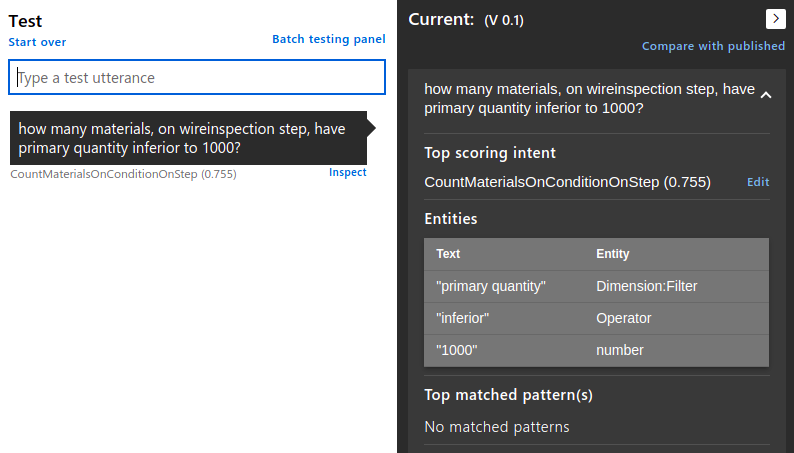
\includegraphics[width=\textwidth]{appendices/assets/nlcomprehension06.png}
        \caption{Intenção \textit{CountOperationsOnConditionOnStepGrouped}}
     \end{subfigure}
\caption{Outras imagens relativas à avaliação de intenções e entidades do protótipo}
\label{fig:nlcomprehesion_others}
\end{figure}

\printglossary
\glsresetall
\end{document}
